\documentclass{sfuthesis}


\title{Multi-Relational Learning with SQL All the Way}
\thesistype{Dissertation}
\author{Zhensong Qian}
\previousdegrees{%
	M.Sc., Shandong University, 2010\\
	B.Sc., Shandong University, 2007}
\degree{Doctor of Philosophy}
\discipline{Computing Science}
\department{School of Computing Science}
\faculty{Faculty of Applied Science}
\copyrightyear{2016}
\semester{Fall 2016}
\date{November-24-2016}

\keywords{Statistical Relational Learning(SRL); Multi-Relational Database; FactorBase; Sufficient Statistics; Log-Linear Model; Bayesian networks (BNs); Dependency Networks (DNs); Link Analysis; Generative Modelling; Discriminative Learning.}

\committee{%
	\chair{Dr. James P. Delgrande}{Professor}
	\member{Dr. Oliver Schulte}{Senior Supervisor\\Professor}
	\member{Dr. Qianping Gu}{Supervisor\\Professor}
	\member{Dr. Jiannan Wang}{Internal Examiner\\Assistant Professor}
	\member{Dr. Xue (Steve) Liu }{External Examiner\\Associate Professor \\ School of Computer Science \\ McGill University}
	
}



\usepackage{amsmath,amssymb,amsthm}
\usepackage[pdfborder={0 0 0}]{hyperref}
\usepackage{graphicx}
\usepackage{caption}
\usepackage{alltt}
\usepackage{array}
\usepackage{amssymb}
\usepackage{float}
%Example for automatically rescaling equations. 
% This is very tricky.
%\begin{equation}
%\label{eq:pimax}
%\resizebox{.55\textwidth}{!}{$
%\begin{split}
%P(\jtable_{2}|\set{E},\ttable) \propto &
%P(\keys = [jack,101],\it{Gr} = A, \it{Sat} = 1|\it{Int} = \class, \it{Rank} = 1, \it{Rat} = 3, \it{Diff}=1)\\
%\times & P(\keys = [jack,102],\it{Gr} = B, \it{Sat} = 2|\it{Int} = \class, \it{Rank} = 1, \it{Rat} = 2, \it{Diff}=2).
%\end{split}$
%}
%\end{equation}

%\usepackage{times}
%\usepackage[normaltitle,normalbib,normalmargins,normalindent]{savetrees}
\usepackage{amsmath}
\usepackage{amsfonts}
\usepackage{amssymb}
\usepackage{graphicx}
\usepackage{url}
%\usepackage{subfigure}
\usepackage{epstopdf}
\setcounter{MaxMatrixCols}{30}
%\usepackage{algorithm}
%\usepackage{algorithmic}
\usepackage{subfigure}
%\usepackage{subcaption}
\usepackage{fancyhdr}
\graphicspath{{../}{figures/}}
\usepackage{todonotes}

\DeclareMathOperator*{\argmax}{argmax}
\DeclareMathOperator*{\argmin}{argmin}
%\DeclareMathOperator{\pattern}{\pi}
\DeclareMathOperator{\Poly}{\mathbf{\mathrm{P}}}
\DeclareMathOperator{\RP}{\mathbf{\mathrm{RP}}}
%\DeclareMathOperator{\FP}{\mathbf{\mathrm{FP}}}
\DeclareMathOperator{\NP}{\mathbf{\mathrm{NP}}}
%\DeclareMathOperator{\E}{\mathbb{E}}
\renewcommand{\d}{\mathbf{d}}

\newcommand{\ZZ}{\mathbf{Z}}

\newcommand{\indep}{\ensuremath{\perp{}\!\!\!\!\!\!\!\perp{}}}
\newcommand{\dep}{\ensuremath{{\perp{}\!\!\!\!\!\!\!\not  \perp{}}}}
%\renewcommand{\L}{\mathcal{L}}
% variables denoting sets of nodes
\newcommand{\V}{V} 
\newcommand{\partC}{\mathcal{C}}
\newcommand{\pattern}{\pi}
% variables denoting nodes
\newcommand{\B}{B}
\renewcommand{\P}{P}
\newcommand{\R}{R}
\newcommand{\X}{X}
\newcommand{\Y}{Y}
\newcommand{\Z}{Z}
\newcommand{\F}{F}
\newcommand{\U}{U}
\newcommand{\W}{W}
\renewcommand{\S}{S}
\newcommand{\C}{C}
\newtheorem{mydef}{Proposition}
%variables for values
%\newcommand{\u}{u}
\renewcommand{\a}{a}
\renewcommand{\b}{b}
\newcommand{\z}{z}
\renewcommand{\v}{v}
\newcommand{\x}{x}
\newcommand{\y}{y}
\newcommand{\p}{p}
\newcommand{\s}{s}
\newcommand{\w}{w} % weights


%statistics
\newcommand{\divergence}{\it{D}}
\newcommand{\score}{\it{score}}
\newcommand{\confidence}{\it{conf}}
\newcommand{\support}{\it{support}}
\newcommand{\loglikelihood}{\it{LOG}}
\newcommand{\lof}{\it{LOF}}
\newcommand{\llmetric}{-L}
\newcommand{\lr}{\it{LR}}
\newcommand{\kl}{\it{KL}}
\newcommand{\el}{\it{EL}}
\newcommand{\mi}{\it{MI}}
\renewcommand{\mid}{\it{ELD}}
\newcommand{\jid}{\it{JID}}
\newcommand{\roc}{\it{ROC}}
\newcommand{\outrank}{\it{OutRank}}
\newcommand{\knn}{\it{KNNOutlier}}
\newcommand{\auc}{\it{AUC}}
\newcommand{\eld}{\it{ELD}}
\newcommand{\fd}{\it{FD}}
\newcommand{\parameter}{\theta}
\newcommand{\parameters}{\bs{\parameter}}
\newcommand{\bic}{\mathit{BIC}}
%random variables and graphical models
% number of values in the domain of a random variable
% variables for BNs
\newcommand{\domvals}{k}
\newcommand{\nodevalue}{\v}
\newcommand{\parvalue}{\mathbf{\pi}} % a single assignment of values to a set of 
%parents
\newcommand{\parvals}{l} % number of values of parent state.
\renewcommand{\r}{r} % CP-table row
\newcommand{\nbhd}{{\mathsf {nbdh}}}
\newcommand{\child}{\mathit{child}}
\newcommand{\parent}{\mathit{pa}}
\newcommand{\parents}{\mathbf{pa}}
\newcommand{\Parents}{\mathbf{PA}}
\newcommand{\family}{F} % families, family formulas
\newcommand{\vpi}{\mathbf{pa}} % for vectors of variable assignments
\renewcommand{\l}{\ell} % class label
\newcommand{\states}{r} % number of states of a variable
%\newcommand{\value}{value}
\newcommand{\mb}{\set{mb}} % markov blanket of a variable, vector-valued
\newcommand{\ssize}{N} % number of rows in join table; size of sample
\newcommand{\mbstates}{m} % number of states in Markov blanket
\newcommand{\frequency}{fr}
\newcommand{\pseudo}{\ast}
\newcommand{\counts}{+}
\newcommand{\weighted}{\ast}
\newcommand{\halpern}{H}
\newcommand{\Thetaa}{\theta}
\newcommand{\instance}{I}

%logic notation
%\newcommand{\predicate}{\phi}
\newcommand{\functor}{f}
\newcommand{\outdomain}{V}
\newcommand{\indomain}{\Omega}
\newcommand{\variable}{X} % first-order variable
\newcommand{\population}{\mathcal{P}}
\newcommand{\entity}{x}
\newcommand{\formula}{\phi}
\newcommand{\formulas}{\mathcal{\phi}}
\newcommand{\literal}{l}
\newcommand{\conjunction}{\set{C}} % conjunction of literals
\newcommand{\fterm}{\f} % open function term
\newcommand{\fterms}{F} % set of function terms, also nodes in JBN
\newcommand{\term}{\sigma}
\newcommand{\Terms}{\bs{\sigma}}
\newcommand{\constant}{a}
\newcommand{\constants}{\bs{\constant}}
\newcommand{\gterm}{g} % ground term
\newcommand{\gterms}{\bs{\gterm}} %list of ground terms
\newcommand{\vterm}{x} % variable term
\newcommand{\vterms}{\bs{\vterm}} % list of variable terms
\newcommand{\assign}{A} % assignment of values to Bayes net
\newcommand{\resultset}{\mathbb{R}}
\newcommand{\grounds}{\#}
\newcommand{\grounding}{\gamma}
\newcommand{\groundall}{\Gamma}
\newcommand{\vars}{\mathit{Var}} % variables in a conjunction
\newcommand{\igraph}{I} % instance-level dependency graph.
\newcommand{\assignment}{\set{a}}
\newcommand{\atom}{\ell}
\newcommand{\gnode}{\alpha}
\newcommand{\gfamily}{\ground{f}}
\newcommand{\numformulas}{m}
\newcommand{\structure}{\mathcal{S}}
% logic programs
\newcommand{\program}{\mathcal{B}}
\newcommand{\clause}{\mathcal{c}}
\newcommand{\head}{\mathit{head}}
\newcommand{\body}{\mathit{body}}
\newcommand{\crule}{\mathit{cr}} % combining rule
\newcommand{\level}{\mathit{level}} % rank of function symbols in LP

%datbase schema
\newcommand{\rcolumns}{R}
\newcommand{\ecolumns}{E}
\newcommand{\dtable}{T} % can't use \table. Generic database table
\newcommand{\datatable}{D} % generic data table, not necessarily part of database.
\newcommand{\jtable}{J} % join table
\newcommand{\Ejoin}{$J^{+}$}
\newcommand{\jtables}{m}
\newcommand{\rtable}{R} % relationship table
\newcommand{\etable}{E} % entity table.
\newcommand{\ttable}{X} % target table
\newcommand{\nextended}{n}
\newcommand{\row}{r}
\newcommand{\rows}{\mathit{rows}}
\newcommand{\col}{j}
\newcommand{\cols}{\mathit{cols}}
\newcommand{\unary}{\f} % to denote a unary or attribute function
\newcommand{\numatts}{u} % to denote the number of unary or attribute functions.
\newcommand{\g}{g} % alternative for function
\newcommand{\relational}{\mathbf{r}} % denotes a generic relational functors, can be both relationship or descriptive attribute of relationship
\newcommand{\Relation}{R} % denotes a generic boolean relation
% a special type of literal conjunction that assigns a value %to each variable
\providecommand{\keywords}{\textbf{keywords: }}
\newcommand{\loss}{\ell}
\newcommand{\class}{c} % the class attribute
\newcommand{\classlabel}{y} % the class label
\newcommand{\classifier}{\mathcal{M}}
\newcommand{\target}{t} % target object
\newcommand{\Target}{T}
\newcommand*\rfrac[2]{{}^{#1}\!/_{#2}}
\newcommand{\object}{o}
\newcommand{\Class}{C}
\newcommand{\scorediff}{\Delta}
\newcommand{\model}{B}
\newcommand{\modelprob}{\theta}
\newcommand{\profile}{P}
% the probabilities defined by a model, like conditional probabilities in a BN
\newcommand{\Targetcount}{\Gamma}
\newcommand{\neighbor}{n}
\newcommand{\feature}{V} % feature or desc attribute of object or link
\newcommand{\features}{\bs{v}} % features 
\newcommand{\Features}{\bs{V}}
\newcommand{\attribute}{a} % nonclass attribute of target object
\newcommand{\attributes}{\bs{a}}
\newcommand{\rels}{\bs{R}} % chain of relationships.
\newcommand{\maxpath}{\rho}
\newcommand{\eatts}{\it{1Nodes}}
\newcommand{\ratts}{\it{2Nodes}}
\newcommand{\atts}{\it{ANodes}}
\newcommand{\marginalize}{\it{margin}}
%special functions
\newcommand{\AVG}{\it{AVG}}
\newcommand{\instances}{n} % counts number of occurrences in DB
\newcommand{\prob}{p} % frequency of formula true in in DB

%variables denoting graphs or models
\newcommand{\mln}{M}
\newcommand{\G}{G}
\newcommand{\node}{V}
\newcommand{\nodes}{V}
\newcommand{\edges}{E}
\newcommand{\clique}{C}
\newcommand{\cliques}{\mathcal{\clique}}
\newcommand{\cliquevalue}{c}
\newcommand{\graph}{G}
\newcommand{\M}{M}
\newcommand{\J}{J}
\renewcommand{\H}{H}
\newcommand{\K}{K} % component
\renewcommand{\O}{O} % oracle
\renewcommand{\path}{\rho} % path, also foreignkey path
% Markov nets
\newcommand{\potential}{\Psi}
% database schema
\newcommand{\type}{\tau} % to denote a generic type
\newcommand{\E}{E} % for entity tables
\newcommand{\e}{e} % for specific entities
\newcommand{\f}{f}
\newcommand{\new}{\it{new}}
\renewcommand{\c}{c}
\renewcommand{\R}{R} % for relationship tables
\newcommand{\A}{A} % for attributes
\newcommand{\T}{T} % for tables generically
\newcommand{\New}{N}
\newcommand{\D}{\mathcal{D}} % for database instance
\newcommand{\databases}{\set{D}} % the number of databases
\newcommand{\vocab}{\mathcal{\L}} % for logical vocabulary associated with database
\newcommand{\name}{\mathit{name}} % generic attribute
\newcommand{\dom}{\mathit{dom}} % domain of attributes
\newcommand{\etables}{\alpha} % entity tables
\newcommand{\rtables}{\beta} % relationship table number
% specific constructs for examples


\newcommand{\team}{\it{T}}
\newcommand{\player}{\it{P}}
\newcommand{\match}{\it{M}}


\newcommand{\director}{\it{Director}}
\newcommand{\movie}{\it{Movie}}
\newcommand{\user}{\it{User}}
\newcommand{\corr}{\it{\rho}}
\newcommand{\student}{\mathit{Student}}
\newcommand{\I}{\mathit{I}}
\newcommand{\course}{\mathit{Course}}
\newcommand{\prof}{\mathit{Professor}}
\newcommand{\person}{\mathit{Person}}
\newcommand{\TA}{\mathit{TA}}
\newcommand{\actor}{\mathit{Actor}}
\newcommand{\age}{\mathit{age}}
\newcommand{\intelligence}{\mathit{intelligence}}
\newcommand{\diff}{\mathit{difficulty}}
\newcommand{\reg}{\mathit{Registered}}
\newcommand{\win}{\it{win}}
\newcommand{\ra}{\mathit{RA}}
\newcommand{\bt}{\mathit{blood type}}
\newcommand{\grade}{\mathit{grade}}
\newcommand{\gpa}{\mathit{gpa}}
\newcommand{\jack}{\mathit{Jack}}
\newcommand{\jill}{\mathit{Jill}}
\newcommand{\smith}{\mathit{Smith}}
\newcommand{\cmpt}{\mathit{CMPT120}}
\newcommand{\hi}{\mathit{Hi}}
% various constants
\newcommand{\true}{\mathit{T}}
\newcommand{\false}{\mathit{F}}
\newcommand{\normalconstant}{Z} % the normalization constant

% orderings
\newcommand{\pred}{\mathit{pred}}
%procedure names and such
\newcommand{\join}{\textsc{Join-Frequencies}}
\newcommand{\linus}{\textsc{Linus }}
\newcommand{\foil}{\textsc{Foil }}
\newcommand{\MLN}{\textsc{MLN}}
\newcommand{\treetilde}{\textsc{TILDE }}

%%%
%undirected models
\newcommand{\pot}{\phi} % potential function
%\newcommand{\theHalgorithm}{\arabic{algorithm}}
\newcommand{\test}{test}
\def\set#1{\mathbf{#1}}
\def\bs#1{\boldsymbol{#1}}
\def\ground#1{\overline{#1}}


\graphicspath{{../../}{figures/}}
\setcounter{tocdepth}{3}

\newcolumntype{R}[1]{>{\raggedleft\let\newline\\\arraybackslash\hspace{0pt}}m{#1}}
\newcommand{\ct}{\mathit{ct}}
\renewcommand{\Qconj}{\Appendterm{\FG{\TT} = \TV} {\QC}} % Use TT instead of \Ground{TI} (TI notation not defined in this paper)
\renewcommand{\marginpar}[1]{\fixneeded{(AS MARGINPAR) #1}}
\newcommand{\fixneeded}[1]{\textbf{[\footnotesize #1]}}
\newcommand{\forcesubsectext}{\hskip 1pt\vskip 0pt\noindent}
\newcommand{\point}[1]{\noindent\emph{#1}.}
\newcommand{\subpoint}[1]{#1:}
\newcommand{\keypoint}[1]{{\em #1}}
\newcommand{\strongpoint}[1]{\paragraph{#1.}}
\newcommand{\iid}{i.i.d.}
\newcommand{\etal}{\textit{et al.}}
\newtheorem{lemma}{Lemma}


\begin{document}

\frontmatter
\maketitle{}
\makecommittee{}

\begin{abstract}
Which doctors prescribe which drugs to which patients? Who upvotes which answers on what topics on Quora? Who has followed whom on Twitter/Weibo? These relationships are all visible in data, and they all contain a wealth of information that could be extracted to be knowledge/wisdom. Statistical Relational Learning (SRL) is a recent growing field which extends traditional machine learning from single-table to multiple inter-related tables. It aims to provide integrated statistical analysis of heterogeneous and interdependent complex data. In the thesis, I focus on modelling the interactions between different attributes and the link itself for such complex heterogeneous and richly interconnected data.
First, I describe the FactorBase system which combines advanced analytics from statistical-relational machine learning (SRL) with database systems. Within FactorBase, all statistical objects are stored as first-class citizens as well as  raw data. This new SQL-based framework pushes the multi-relational model discovery into a relational database management system. Secondly, to solve the scalability issue of computing cross-table sufficient statistics, a new Virtual Join algorithm is proposed and implemented in FactorBase. Bayesian networks (BNs) and Dependency Networks (DNs) are two major classes of SRL. Thirdly, I utilize FactorBase to extend the state-of-the-art learning algorithm for BN of generative modelling with link uncertainty. The learned model captures correlations between link types, link features, and attributes of nodes, simultaneously. Finally, a fast hybrid approach is proposed for instance level discriminative learning of DNs with competitive predictive power but substantially better  scalability.

\end{abstract}


\begin{dedication} 
To my wife, parents and sisters  for their constant support and unconditional love.
\end{dedication}


\begin{acknowledgements} 
Firstly, I would like to express  special appreciation and thanks to my senior supervisor Dr. Oliver Schulte, for his continuous support, great patience,  encouraging motivation, and immense knowledge during my Ph.D. study at Simon Fraser University. Oliver has been a tremendous mentor for me, both professionally and personally. His advices on research as well as on my career have been priceless. I could not have imagined having a better senior supervisor and mentor.

Besides my senior supervisor, I would also like to thank  the rest of my committee members. I am grateful to Dr. Qianping Gu for his  constructive suggestions and personal encouragement throughout my entire Ph.D. study.  I appreciate Dr. Jiannan  Wang for his insightful comments and feedback.  It is a great honor to have Dr. Xue (Steve) Liu as my external examiner. I am also thankful to Dr. James P. Delgrande  for serving as the chair of my committee.

I consider myself very lucky to have the chance to collaborate with so many wonderful people who helped me to accomplish the results descripted in this thesis. 
I am very grateful to all my collaborators. I would also like to thank all of my friends and labmates (too many to list here but you know who you are) who supported me in writing, and incented me to strive towards my goal. I  greatly appreciate the administrative and technical staff members of the school of Computing Science who have been kind enough to advise and help in their respective roles. My life would not be so enjoyable without your sharing, blessing and encouragement.


Last but not the least, I owe my deepest thanks to my family: my parents, my sisters and my wife. I know I always have my family to count on during a challenging period. My hard-working parents have sacrificed their lives for my sisters and myself and provided unconditional life-time love and care. My sisters for listening to my compliants, for their understanding and for believing in me.  A very special heartfelt thanks to my wife Yanqin Liu, for her love, support and encouraging me to follow my dream. Words cannot express my gratitude for all the sacrifices they have made on my behalf. This dissertation is impossible without their love and support.


\end{acknowledgements}

\addtoToC{Table of Contents}\tableofcontents\clearpage
\addtoToC{List of Tables}\listoftables\clearpage
\addtoToC{List of Figures}\listoffigures


\mainmatter%

\chapter{Introduction }\label{sec:intro}

Many real world datasets are relational and most real world applications are characterized by the presence of uncertainty and complex relational structures (see an example in Figure \ref{fig:RelationalSocialMedia1} of the domain of online social media). Using interconnected information as the input provides a richer knowledge to the machine and helps the process of learning. The domains often consist of a variety of object types; the interactions between these objects can be linked  into multiple types as well. A university network may consist of several kinds of object like students, professors and courses, as well as the interactions, such as teaching, course registration or research assistant relationship. Similar types of instances are ubiquitous, from online social media to scientific research publication networks,  public health care systems, and to electrical power grids, and so on. To tackle the interesting yet critical problem of modelling such heterogeneous data, appropriate care must be taken due to the correlations of features and/or different kinds of links \cite{Sun2012}: attributes of linked objects are often correlated, and links are more likely to exist between objects that share similar attributes. In the thesis, I focus on  modelling the interactions between different attributes and the link itself for complex heterogeneous and richly interconnected data.

\begin{figure*}[!h] 
   \centering
      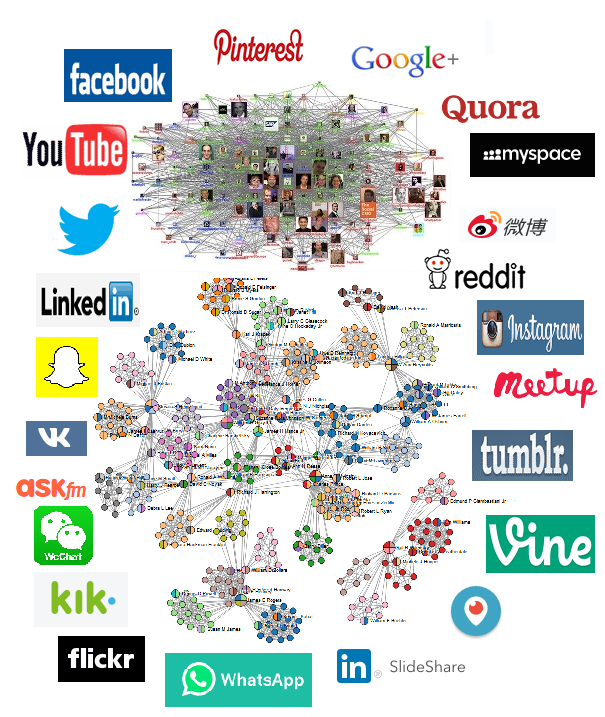
\includegraphics[width=0.9\textwidth]{socialGraph.png} 
   \caption{Example of interconnected online social media. %Courtesy of Lise Getoor.
}
   \label{fig:RelationalSocialMedia1}
\end{figure*}


\section{Multi-Relational Data Representation}
The choice of an appropriate representation is  an important issue which has a significant impact on the quality of the statistical inferences that can be made. The structure of interrelated/relational data presents an opportunity for objects to carry additional information via their links and enables the model to show correlations among objects and their relationships. 
With the current surroundings,  the general {\em entity} and {\em relationship} (ER) diagram from the database community is a powerful and expressive representation of the complex real-world interactions between multiple kinds of objects and links in diverse domains. Additionally   techniques provided by the relational database management system(RDBMS) can be leveraged for manipulating data as well as models. 


\begin{figure}[!h] 
 \centering
\resizebox{1\textwidth}{!}{
 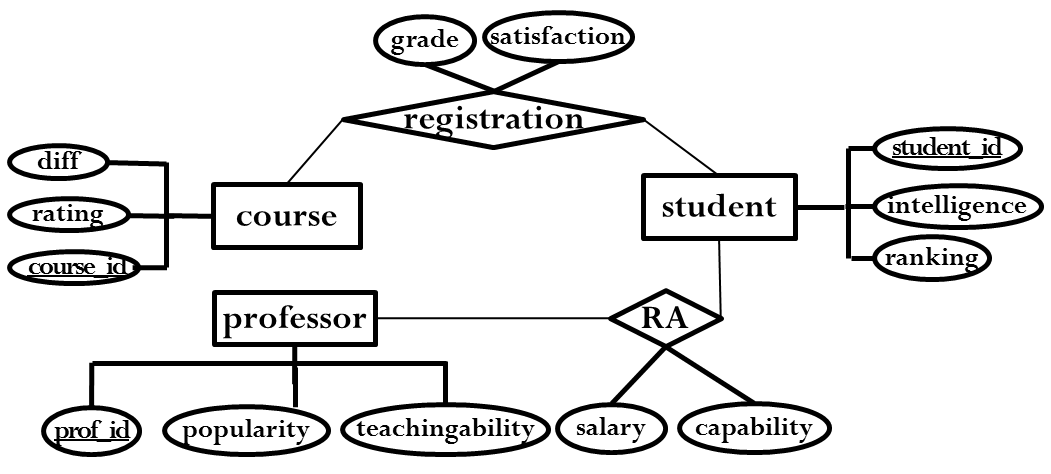
\includegraphics[width=0.9\textwidth]{university-schema.png}
} 
\caption{A relational ER Design. Registration and RA are many-to-many relationships.}
 \label{fig:university-schema}
\end{figure} 

\begin{figure}[htbp] %  figure placement: here, top, bottom, or page
 \centering
\resizebox{1\textwidth}{!}{
 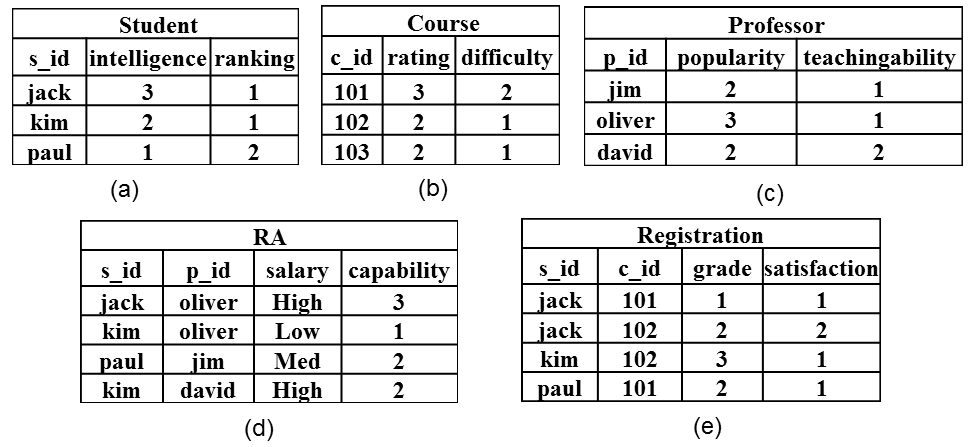
\includegraphics[width=0.9\textwidth]{university-tables.png} 
}
\caption{Database Instance based on Figure~\ref{fig:university-schema}.  
}
 \label{fig:university-tables}
\end{figure}
In the following chapters, I will assume the format data is represented as an ER diagram.
A standard \textbf{relational schema} contains a set of tables, each with key fields,  descriptive attributes, and possibly foreign key pointers.  The tables in the relational schema can be divided into {\em entity tables} and {\em relationship tables} \cite[Ch.2.2]{Ullman1982}. An ER diagram shows entity sets as boxes, relationships between entities as diamonds, and attributes as ovals.

Figure \ref{fig:university-schema} shows a relational diagram for a database related to a university which contains three objects or entity tables:  $\student$,  $\course$, and $\prof$, and two relationship tables; $\reg$ with foreign key pointers to the $\student$ and $\course$ tables whose tuples indicate which students have registered in which courses and $\ra$ with foreign key pointers to the $\student$ and $\prof$ tables whose tuples indicate the RAship of students for professors. 
Relationships refer to their related objects using \textit{reference slots}. Each table in the relational database is seen as a class that has some descriptive attributes.
A \textbf{database instance} specifies the tuples contained in the tables of a given database schema. Figure \ref{fig:university-tables} is an instance for the schema in Figure \ref{fig:university-schema}.


\section{Log-linear Template Models for Relational Data} \label{sec:log-linear}
As illustrated in Figure \ref{fig:relVan}, statistical relational learning (known as SRL) is a recent growing field. It is the intersection of artificial intelligence, machine learning and database systems. SRL extends traditional machine learning from single-table to multiple inter-related tables. It aims to provide integrated statistical analysis of the complex data sources.  The extensive survey by Kimmig {\em et al.} \cite{Kimmig2015}  shows that  SRL models can be viewed as log-linear models based on ``parametrized factor'' as follows. 
Par-factor stands for ``parametrized factor''. 
A par-factor represents an interaction among parametrized random variables, or par-RVs for short. In this section, I review the background knowledge from log-linear models to motivate my thesis work. In section \ref{sec:examples}, I show the Parametrized Bayesian Network as one example among the SRL models and introduce the structure learning algorithm in section \ref{sub:sla}. In the following chapters of my thesis, I consider ``Bayesian Network''  and  ``Bayes Net'' the same term, and I use them  interchangeablely.

\begin{figure}[htbp] %  figure placement: here, top, bottom, or page
 \centering
  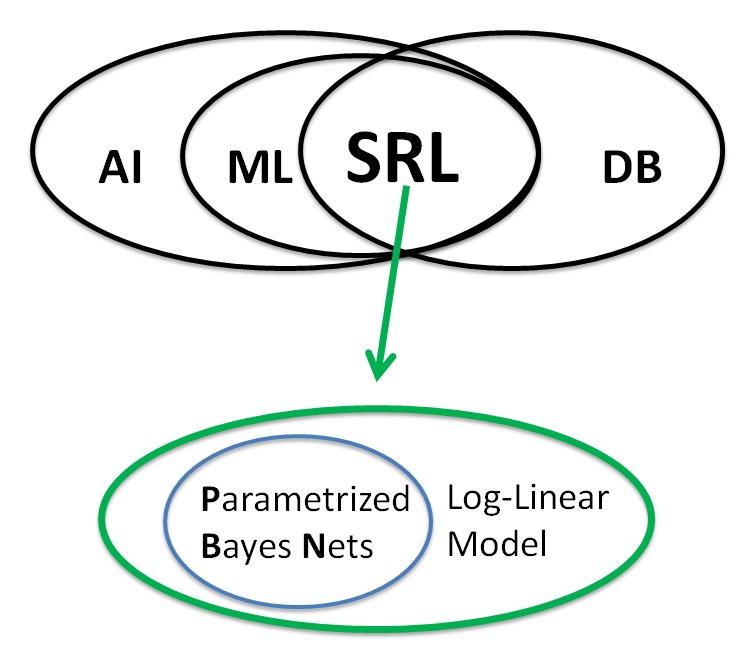
\includegraphics[width=0.45\textwidth]{relVan.png} 
	\caption{ SRL is the intersection of artificial intelligence (AI), machine learning (ML) and database systems (DB).  Parametrized Bayesian Network is one the SRL models that can be viewed as log-linear models.\label{fig:relVan}}  
\end{figure}

The concept of a parametrized random variable (par-RV) marries logical-relational notation to a statistical concept. I employ the following notation for par-RVs \cite[2.2.5]{Kimmig2015}.	Constants are expressed in lower-case, e.g. $\it{joe}$, and are used to represent entities. A type is associated with each entity, e.g. $\it{joe}$ is a person. 
A first-order variable is also typed, e.g. $\it{Person}$ denotes some member of the class of persons. A functor maps a tuples of entities to a value. I assume that the range of possible values is finite.  An {\em atom} is an expression of the form $r(\term_{1},\ldots,\term_{a})$ where each $\term_{i}$ is either a constant or a first-order variable. If all of $\term_{1},\ldots,\term_{a}$ are constants, $r(\term_{1},\ldots,\term_{a})$ is a {\em ground atom} or random variable (RV), otherwise a {\em first-order atom} or a \textbf{par-RV}. A par-RV is instantiated to an RV by grounding, i.e. substituting a constant of the appropriate domain for each first-order variable. 

A \textbf{par-factor} is a pair $\parfactor = (\parrvs,\potential)$, where $\parrvs$ is a set of par-RVs, and $\potential$ is a function from the values of the par-RVs to the non-negative real numbers.\footnote{A par-factor can also include constraints on possible groundings.} Intuitively, a grounding of a par-factor represents a set of ground random variables that interact with each other locally. SRL models use {\em parameter tying}, meaning that if two groundings of the same par-factor are assigned the same values, they return the same factor value. A set of parfactors $\parfactors$ defines a joint probability distribution over the ground par-RVs as follows. Let $\instantiations(\parfactor_{i})$ denote the set of {\em all} ground par-RVs in par-factor $\parfactor_{i}$. Let $\set{x}$ be a joint assignment of values to all ground random variables. Notice that this assignment determines the values of all ground atoms. An assignment $\set{X}=\set{x}$ is therefore {\em equivalent to a single database instance}.
%, or a possible world. 
The probability of a database instance is given by the log-linear equation \cite[Eq.7]{Kimmig2015}:
\begin{equation} \label{eq:parfactor}
P(\set{X}=\set{x}) = \frac{1}{Z} \prod_{\parfactor_{i} \in \parfactors} \prod_{\gparrvs \in \instantiations(\parfactor_{i})} 
\potential_{i}(\set{x}_{\gparrvs}) 
\end{equation}
where $\set{x}_{\gparrvs}$ represents the values of those variables in $\gparrvs$ that are necessary to compute $\potential_{i}$. 
Equation~\ref{eq:parfactor} can be evaluated, without enumerating the ground par-factors, 
as follows. 
(1) For each par-factor, for each possible assignment of values, find the number of ground factors with that assignment of values. (2) Raise the factor value for that assignment to the number of instantiating factors. (3) Multiply the exponentiated factor values together.  The number (2) of ground factors with the same assignment of values is known as a \textbf{sufficient statistic}.



\begin{figure}[htbp] %  figure placement: here, top, bottom, or page
 \centering
\resizebox{0.9\textwidth}{!}{
 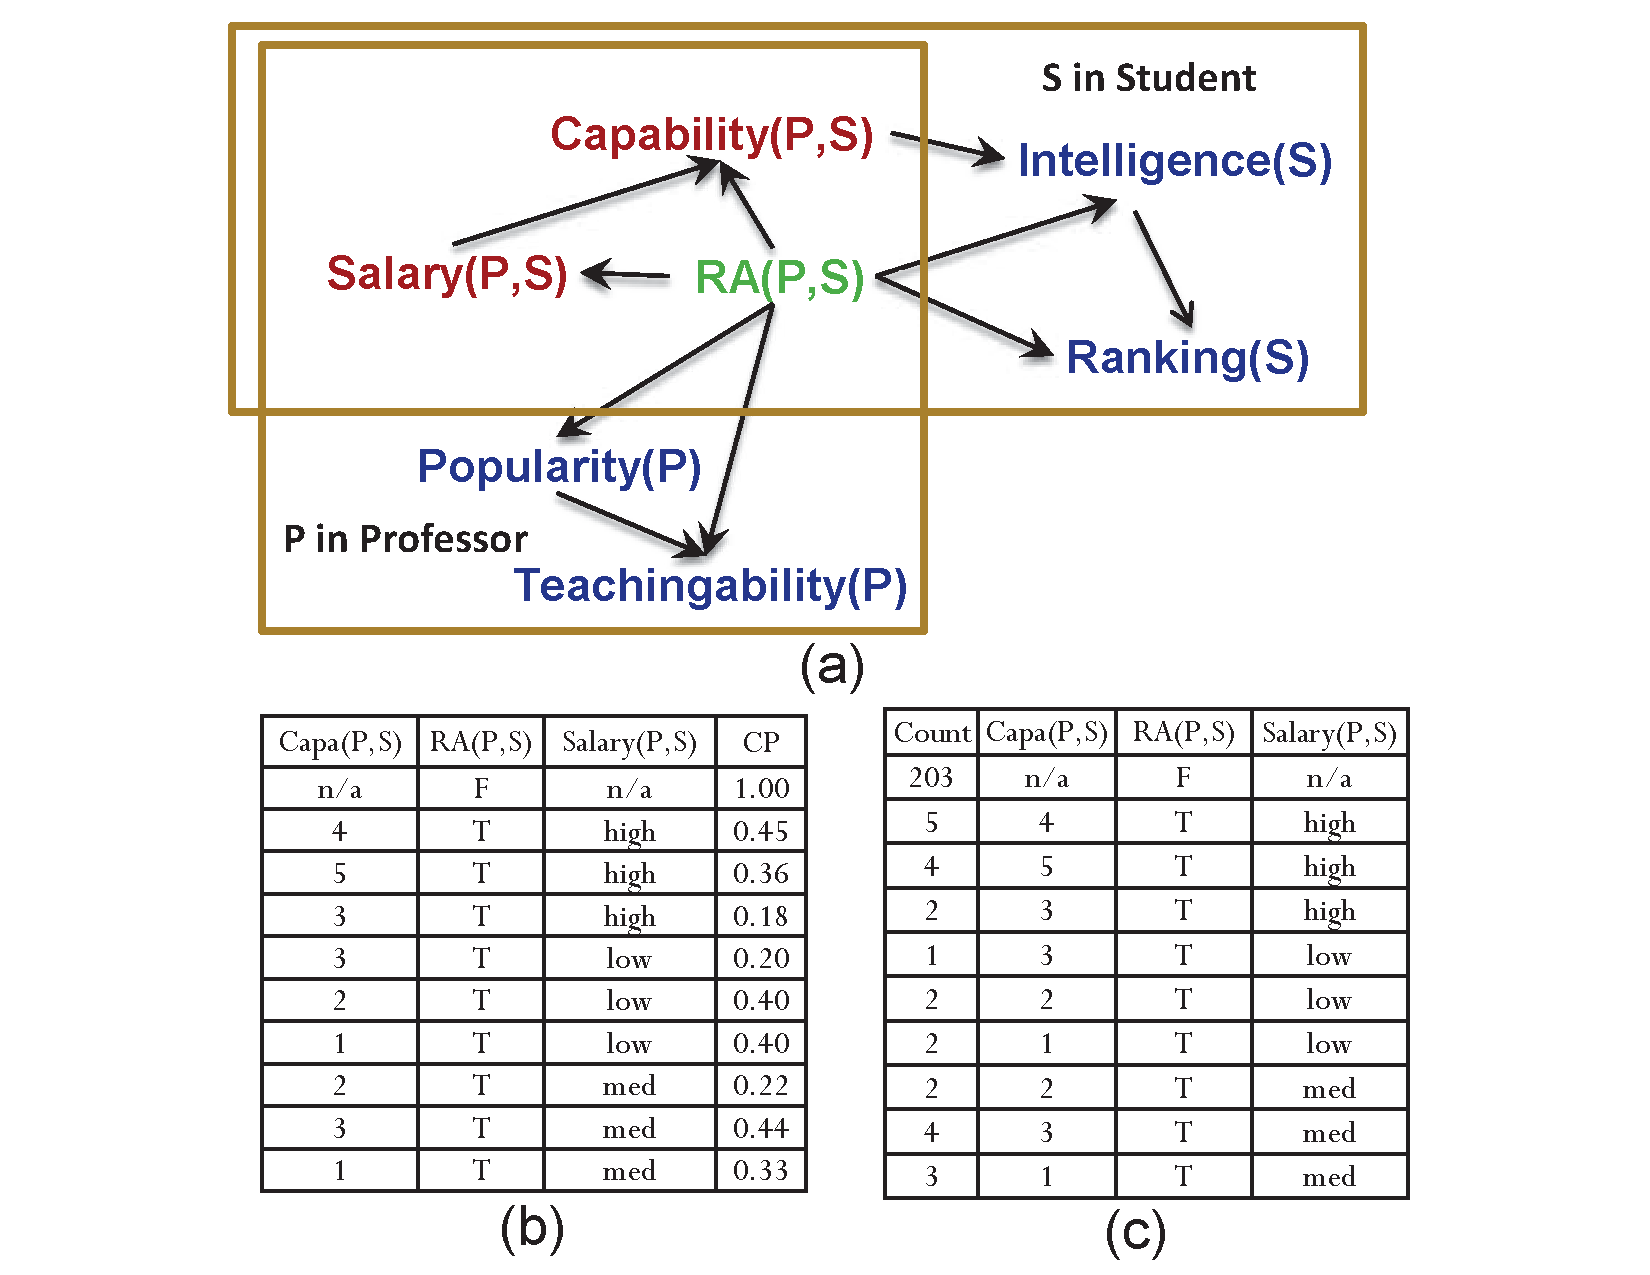
\includegraphics{pbn.pdf} 
} 
\caption{(a) Bayesian network for the University domain. I  omit the $\reg$ relationship for simplicity. The network was learned from the University dataset \cite{bib:bbsite}.
(b) Conditional Probability Table $Capability(\P,\S)\_\cptable$, for the node $Capability(\P,\S)$. Only value combinations that occur in the data are shown. This is an example of a factor table. (c) Contingency Table $Capability(\P,\S)\_\cttable$ for the node $Capability(\P,\S)$ and its parents. Both CP and CT tables are stored in an RDBMS.}
 \label{fig:pbn}
\label{fig:ct-cp-table}
\end{figure}

\subsection{Examples: Parametrized Bayesian Network} \label{sec:examples} 
SRL has developed a number of formalisms for describing par-factors \cite{Kimmig2015}. 
First-order probabilistic graphical models
are popular both within SRL and the database community \cite{Kimmig2015,Wang2008}. The model structure is defined by edges connecting par-RVs. For instance, a \textbf{parametrized Bayesian network structure} is a directed acyclic graph (DAG) whose nodes are par-RVs.  Figure \ref{fig:pbn} shows a Bayesian network for a University domain. 
The schema for the university domain is given in Figure~\ref{fig:university-schema}. This schema features only one relationship for simplicity; FactorBase  learns a model for any number of relationships. While I  describe FactorBase  abstractly in terms of par-factors, for concreteness I  illustrate it using Bayesian networks. The system takes as input a database instance like that shown in Figure~\ref{fig:university-tables}, and produces as output a graphical model like that shown in Figure~\ref{fig:pbn} (a).  



A par-factor in a Bayesian network is associated with a \textbf{family} of nodes \cite[Sec.2.2.1]{Kimmig2015}. A family of nodes comprises a child node and all of its parents. For example, in the BN of Figure~\ref{fig:pbn}, one of the par-factors is associated with the par-RV set
 $$\parrvs=\{\it{Capability}(\P,\S),\it{Salary}(\P,\S),\it{RA}(\P,\S)\}.$$ 
 For the database instance of Figure~\ref{fig:university-tables}, there are $3\times3=9$ possible factors associated with this par-RV, corresponding to the Cartesian product of 3 professors and 3 students. The value of the factor $\phi$ is a function from an assignment of family node values to a non-negative real number. \textbf {In a Bayesian network, the factor value represents the conditional probability of the child node value given its parent node values.} These conditional probabilities are typically stored in a table as shown in Figure~\ref{fig:pbn}(b). This table represents therefore the function $\phi$ associated with the family par-factor. Assuming that all par-RVs have finite domains, a factor can always be represented by a \textbf{factor table} of the form Figure~\ref{fig:pbn}(b): there is a column for each par-RV in the factor, each row specifies a joint assignment of values to a par-RV, and the factor column gives the value of the factor for that assignment (cf. \cite[Sec.2.2.1]{Kimmig2015}).



The sufficient statistics for the $\it{Capability}(\P,\S)$ family can be represented in a contingency table as shown in Figure~\ref{fig:pbn}(c). For example, the first row of the contingency table indicates that the conjunction $\it{Capability}(\P,\S)=n/a,\it{Salary}(\P,\S)=n/a,\it{RA}(\P,\S) =\false$ is instantiated 203 times in the University database (publicly available at~\cite{bib:bbsite}). This means that for 203 professor-student pairs, the professor did not employ the student as an RA (and therefore the salary and capability of this RA relationship is undefined or $n/a$).

\subsection{SRL Structure Learning}\label{sub:sla}

Algorithm~\ref{alg:learning} shows the generic format of a statistical-relational structure learning algorithm (adapted from 
\cite{Kimmig2015}%Kimming and Getoor
). The instantiation of procedures in lines 2, 3, 5 and 8 determines the exact behavior of a specific learning algorithm. The structure algorithm carries out a local search in the hypothesis space of graphical relational models. A set of candidates is generated based on the current model (line 3), typically using a search heuristic. For each candidate model, parameter values are estimated that maximize a model selection score function chosen by the  user (line 5). A model selection score is computed for each model given the parameter values, and the best-scoring candidate model is selected (line 7). 



\begin{algorithm}[!h] 
\KwIn{Hypothesis space $ \mathcal H$ (describing graphical models), training data $\mathcal D$ (assignments to random variables), scoring function score ($\cdot$, $\mathcal D$)}
\KwOut{A graph structure $G$ representing par-factors.}
\begin{algorithmic}[1]
\STATE $G \leftarrow 	\emptyset$
\WHILE{ \textsc{continue}($G$, %$h$, 
$\mathcal H$, score ($\cdot$, $\mathcal D$) )} 
	\STATE{ $\mathcal R \leftarrow $ \textsc{refine}C\textsc{andidates}($G, \mathcal H$)} 
 	\FORALL{$R \in \mathcal R$} 
		\STATE{$R \leftarrow$ \textsc{learn}P\textsc{arameters}($R$,score ($\cdot$, $\mathcal D$))} 
    \ENDFOR
	\STATE 	$G \leftarrow$ argmax$_{G^{\prime} \in \mathcal R\cup \{G\}}$ score($G^{\prime} $, $\mathcal D$)

\ENDWHILE

\STATE \Return $G$
\end{algorithmic}

\caption{Structure learning algorithm (instantiation of procedures in lines 2, 3, 5 and 8 determines exact behaviour) 
\label{alg:learning}}
\end{algorithm}




\section{Related Work} \label{sec:related}
I design the FactorBase system  which combines advanced analytics from multi-relational or statistical-relational machine learning (SRL) with database systems. 
This new SQL-based framework uses the RDBMS to manage the learned model  as first-class citizen and the relational data so that one can leverage the RDBMS to support the multi-relational model discovery.
 In chapter \ref{cha:system}, I  will discuss the system design details and show how it supports model discovery algorithms that follow Algorithm~\ref{alg:learning}. Figure~\ref{fig:architecture} outlines the system components and dependencies among them. The design space for combining machine learning with data management systems offers a number of possibilities, several of which have been explored in previous and ongoing research. I  selectively review the work most relevant to my research and the FactorBase system. Figure~\ref{fig:related} provides a graphical illustration of where FactorBase is located with respect to other works.

\begin{figure}[!h] %  figure placement: here, top, bottom, or page
 \centering
  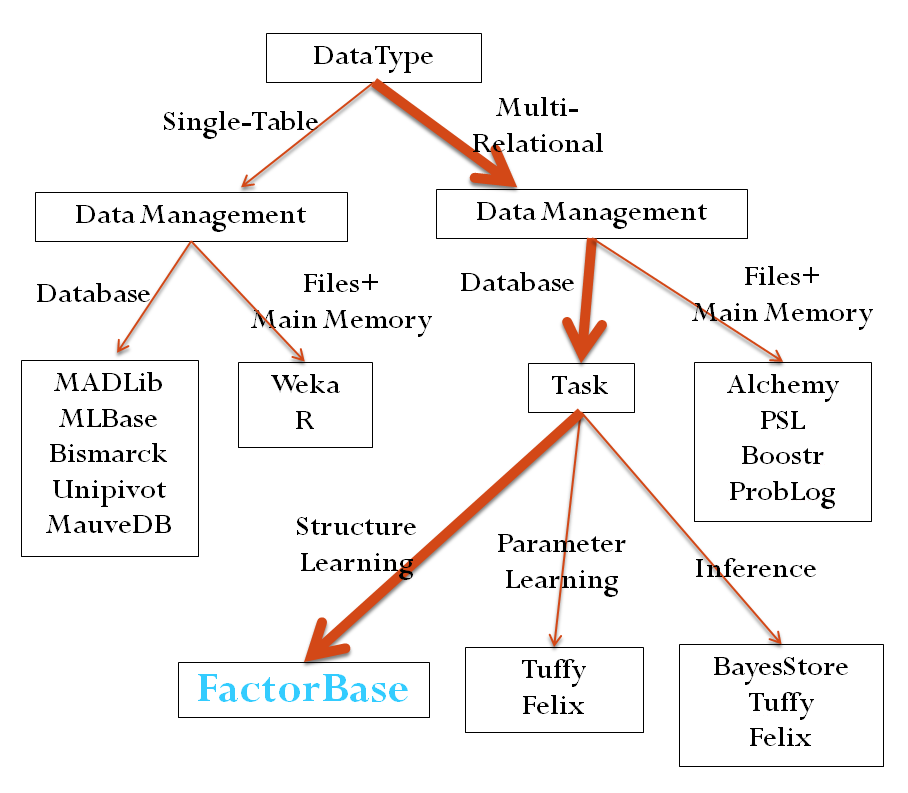
\includegraphics[width=1\textwidth]{related-dt.png} 
\caption{A tree structure for related work in the design space of machine learning $\times$ data management.}
\label{fig:related}
\end{figure}

\subsection{Single-Table Machine Learning} 
Most machine learning systems, such as Weka or R, support learning from a single table or data matrix only. The single-table representation is appropriate when the data points represent a homogeneous class of entities with similar attributes, where the attributes of one entity are independent of those of others \cite{Kimmig2015}. The only way a single-table system can be applied to multi-relational data is after a preprocessing step where multiple interrelated tables are converted to a single data table. When the learning task is classification, such preprocessing is often called propositionalization  \cite{Kimmig2015}.  This ``flattening'' of the relational structure typically involves information loss.  

\paragraph{RDBMS Learning}
Leveraging RDBMS capabilities through SQL programming has been explored for a variety of single-table learning tasks. This is the unifying idea of the recent MADLib framework \cite{MADlib_VLDB_2012}. An advantage of the MADLib approach that is shared by FactorBase  is that in-database processing avoids exporting the data from the input database. The Apache Spark \cite{Committers} framework includes MLBase and SparkSQL that provide support for distributed processing, SQL, and automatic refinement of machine learning algorithms and models~\cite{MLbase_ICDR_2013}.
Other RDBMS applications include gathering sufficient statistics \cite{Graefe1998}, and convex optimization \cite{Feng_SIGMOD_2012}. The MauveDB system \cite{Deshpande2006} emphasizes the importance of several RDBMS features for combining statistical analysis with databases.
As in {\sc FactorBase}, this includes 
storing models and associated parameters as objects in their own right, 
and using the view mechanism to update statistical objects as the data change.
A difference is that MauveDB presents model-based views of the {\em data} to the user, whereas FactorBase  presents views of the {\em models} to machine learning applications. 

\paragraph{RDBMS Inference}
Wong {\em et al.}  applied SQL operators such as the natural join to perform log-linear inference with a single-table graphical model \cite{Wong1995} stored in an RDBMS. 
Monte Carlo methods have also been implemented with an RDBMS  to perform inference with uncertain data~\cite{MCDB_SIGMOD_2008,Wick_VLDB_2010}.
The MCDB system \cite{MCDB_SIGMOD_2008}  stores parameters in database tables like FactorBase. 


\paragraph{Parameter Server (PS) paradigm } %: cite Steve Liu??
For scaling up machine learning to large datasets and complex problems, distributed optimization and inference mechanism have been increasingly popular and a variety of approaches have been proposed \cite{Bekkerman2011}. Several related systems,  including open source projects have been implemented at Google \cite{Dean2012}, Yahoo \cite{Ahmed2012} and Petuum \cite{Ho2013}. The PS framework (globally shares the parameters by scheduling the workload of storing and updating large volume of parameters to distributed servers) was first introduced by Smola et al \cite{Smola2010} and it has proliferated in both industrial and academic research communities \cite{Li2014}. There are also some critical issues arised as it moves forward \cite{Nan2015}.
The PS paradigm could be considered as general-purpose framework, it focuses on improving the ``systems'' code (notably, communication and synchronization protocols for model state) to increase the efficiency of machine learning algorithms \cite{Dai2015}. 
In contrast, the FactorBase System combines both systems code improvements and algorithmic learning improvements tailor-made for log-linear model of multi-relational data.
The PS paradigm can be used to perform inference on the log-linear template model once it is learned, and potentially it could be integrated into Model Manager as introduced in section \ref{sec:mod}.

\subsection{Multi-Relational Learning} 
For overviews of multi-relational learning please see \cite{SRL2007,Domingos2009,Kimmig2015}. Most implemented systems, such as Aleph and Alchemy, use a logic-based representation of data derived from Prolog facts, that originated in the Inductive Logic Programming community \cite{Dzeroski2001c}. 

\paragraph{RDBMS Learning}
The ClowdFlows system \cite{Lavravc2014} allows a user to specify a MySQL database as a data source, then converts the MySQL data to a single-table representation using propositionalization. 
Singh and Graepel \cite{Singh2013} present an algorithm that analyzes the relational database system catalog to generate a set of nodes and a Bayesian network structure. 
This approach utilizes SQL constructs as a data description language in a way that is similar to the schema analyzer which will be introduced in section \ref{chaSecRVD}. 
Differences include the following. (1) The Bayesian network structure is fixed and based on latent variables, rather than learned for observable variables only, as in the case study. (2) The RDBMS is not used to support learning after random variables have been extracted from the schema. 


Qian {\em et al.} \cite{Qian2014a}  discuss work related to the contingency table problem and introduce contingency table algebra. Their paper focuses on a Virtual Join algorithm for computing sufficient statistics that involve negated relationships. They do not discuss integrating contingency tables with other structured objects for multi-relational learning. 
%

\paragraph{RDBMS Inference} 
Database researchers have developed powerful probabilistic inference  algorithms for multi-relational models. 

 The BayesStore system \cite{Wang2008} introduced the principle of treating all statistical objects as first-class citizens in a relational database as FactorBase  does. The Tuffy system \cite{Niu2011} achieves highly reliable and scalable inference for Markov Logic Networks (MLNs) with an RDBMS. It leverages inference capabilities to perform MLN parameter learning. RDBMS support for local search parameter estimation procedures, rather than closed-form maximum-likelihood estimation, has also been explored \cite{Feng_SIGMOD_2012,Niu2011,Niu2011a}.


\section{Contributions}
Within this section, I highlight  the contributions of my thesis evaluated with respect to scalability, quality and other performance criterion (e.g. preprocessing time, usefulness) as follows.

\paragraph {FactorBase} In chapter \ref{cha:system}, I describe the FactorBase system which combines advanced analytics from multi-relational or statistical-relational machine learning (SRL) with database systems. This new SQL-based framework pushes the multi-relational model discovery into a relational database management system.  Empirical evaluation shows significant scalability advantages from utilizing the RDBMS capabilities: Both structure and parameter learning scale well to millions of data records, beyond what previous multi-relational learning systems can achieve.  This work has been reported in \cite{Qian2015, Zhensong2015}.

\paragraph {Cross-table Sufficient Statistics} For most of the learning task, the scalability bottleneck is to compute the cross-table sufficient statistics.  In chapter \ref{cha:multiStatistic}, I propose and implemente in FactorBase a new Virtual Join algorithm  to tackle this problem.  Empirical evaluation demonstrates the scalability of the algorithm and illustrates how access to sufficient statistics for both positive and negative relationships enhances feature selection and rule mining. This provides the evidence of the statistical quality and usefulness of the sufficient statistics computed by the Virtual Join algorithm. This work has been reported in \cite{Qian2014a,  Qian2014}.

\paragraph  {Generative modelling with Link Uncertainty} %To evaluate the usefulness of the system, 
I incorporate the FactorBase system to tackling challenge applications. In chapter \ref{cha:lbn}, I utilize FactorBase system as a pre-counting approach on gathering sufficient statistics to extend the state-of-the-art learning algorithm for Bayes net generative modelling of multiple links considering link uncertainty. The extended algorithm supports  to capture simultaneous correlations between link types, link features, and attributes of nodes. This type of model supports queries like, ``What fraction of the grades are awarded to highly intelligent students?'' The empirical study illustrates the usefulness of the proposed model with respect to find additional correlations among different types of links. This work has been reported in \cite{Qian_LNAI_2014, Qian2014}.

\paragraph {Instance Level Discriminative Learning}% 
Bayes nets and Dependency networks (DNs) are two major classes of Statistical Relational Learning (SRL).  In chapter \ref{cha:RDN},  I propose a fast scalable hybrid approach for instance level discriminative learning of DNs.  This type of model supports queries like, ``What is the probability of {\em Jack} being a highly intelligent student given the grades of his registered courses?'' The experiment shows that the predictive power with respect to statistical accuracy of the model learned with the hybrid learning algorithm
is competitive with those from state-of-the-art function gradient boosting methods but scales substantially better than the boosting methods. This work has been reported in \cite{Schulte2014a, Schulte2016}.


\section{Thesis Organization}
The organization of this thesis is as follows. 
First, in Chapter \ref{sec:intro}, I review the background from multi-relational data representation of log-linear models and structure learning to motivate my thesis work, followed by related works in the field.  And then I describe  the design principles and key components of FactorBase system in Chapter \ref{cha:system}. The new Virtual Join algorithm for cross-table sufficient statistics computation to tackle the learning bottleneck is introduced in Chapter \ref{cha:multiStatistic}.
Following in Chapter \ref{cha:lbn} and Chapter \ref{cha:RDN}, I conduct the usefulness evaluation of the system with generative and discriminative modelling, respectively.
Finally, Chapter \ref{cha:lim} concludes this thesis, identifies limitations of the proposed system and methods, and discusses possible directions for future work. 

\chapter{FactorBase: a new SQL-based framework for multi-relational model discovery} \label{cha:system}



The system described in this chapter combines advanced analytics from multi-relational or {\em statistical-relational} machine learning (SRL) with database systems. The power of combining machine learning with database systems has been demonstrated in several systems\cite{MADlib_VLDB_2012,MLbase_ICDR_2013,Deshpande2006}.
The novel contribution of FactorBase  is supporting machine learning for {\em multi-relational} data, rather than for traditional learning where the  data are represented in a {\em single} table or data matrix. 

I  discuss new challenges raised by multi-relational model learning compared to single-table learning, and how FactorBase  solves them using the resources of SQL (Structured Query Language). The name FactorBase  indicates that the system supports learning factors that define a log-linear multi-relational model~\cite{Kimmig2015}. Supported new database services include constructing, storing, and transforming complex statistical objects, such as factor-tables, cross-table sufficient statistics, parameter estimates, and model selection scores.
My argument is that relational algebra can play the same role for statistical-relational learning that linear algebra does for traditional single-table machine learning:  a unified language for both representing and computing with statistical-relational objects. 



\section{Introduction} 

FactorBase  is the first system that leverages relational query processing for learning a multi-relational log-linear graphical model. Whereas the in-database design philosophy has been previously used for multi-relational inference, I am the first to adapt it for multi-relational model structure learning. 
The experiments show that FactorBase  pushes the scalability boundary: Learning scales to databases with over $10^6$ records, compared to less than $10^5$ for previous systems. At the same time it is able to discover more complex cross-table correlations than previous SRL systems. I  report experiments that focus on two key services for an SRL client: (1) Computing and caching sufficient statistics, (2) computing model predictions on test instances. For the largest benchmark database, the system handles 15M sufficient statistics. 
SQL facilitates block-prediction for a set of test instances, which leads to a 10 to 100-fold speedup compared to a simple loop over test instances.

Pushing the graphical model inside the database allows us to {\em use SQL as a high-level scripting language for SRL}, with the following advantages.

\begin{enumerate}
\item Extensibility and modularity, which support rapid prototyping. SRL algorithm development can focus on statistical issues and rely on a RDBMS for data access and model management.
\item Increased scalability, in terms of both the size and the complexity of the statistical objects that can be handled.
\item Generality and portability: standardized database operations support ``out-of-the-box'' learning with a minimal need for user configuration.
\end{enumerate}
\paragraph{Chapter Organization}
I  first provide an overview of the system components and the work flow in Figure \ref{fig:architecture}. And for each component, I  describe how the component is constructed and managed inside an RDBMS using SQL scripts and the SQL view mechanism. I  show how the system manages sufficient statistics and test instance predictions in a block access way. The evaluation section demonstrates the scalability advantages of in-database processing. 


%
\begin{figure*}[t]
\begin{center}
\resizebox{1\textwidth}{!}{
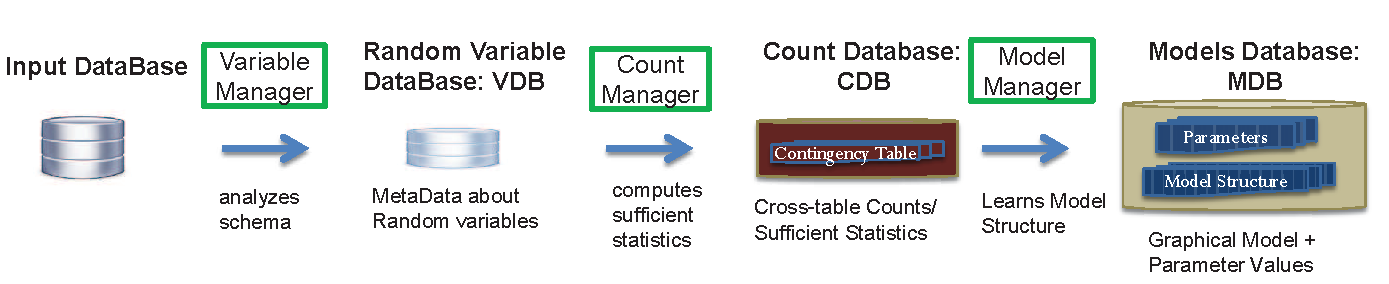
\includegraphics{pipeline}
}
\caption{System Flow. All statistical objects are stored as first-class citizens in a DBMS. Objects on the left of an arrow are utilized for constructing objects on the right. Statistical objects are constructed and managed by different modules, shown as boxes. 
\label{fig:architecture}}
\end{center}
\end{figure*}


\section{The Random Variable Database} \label{chaSecRVD}

Statistical-relational learning requires various metadata about the par-RVs in the model. These include the following. 

\begin{description}
\item[Domain] the set of possible values of the par-RV.
\item[Types] Pointers to the first-order variables in the par-RV. 
\item[Data Link] Pointers to the table and/or column in the input database associated with the par-RV. 
\end{description}


\begin{figure}[h] %  figure placement: here, top, bottom, or page
 \centering
\resizebox{0.8\textwidth}{!}{
 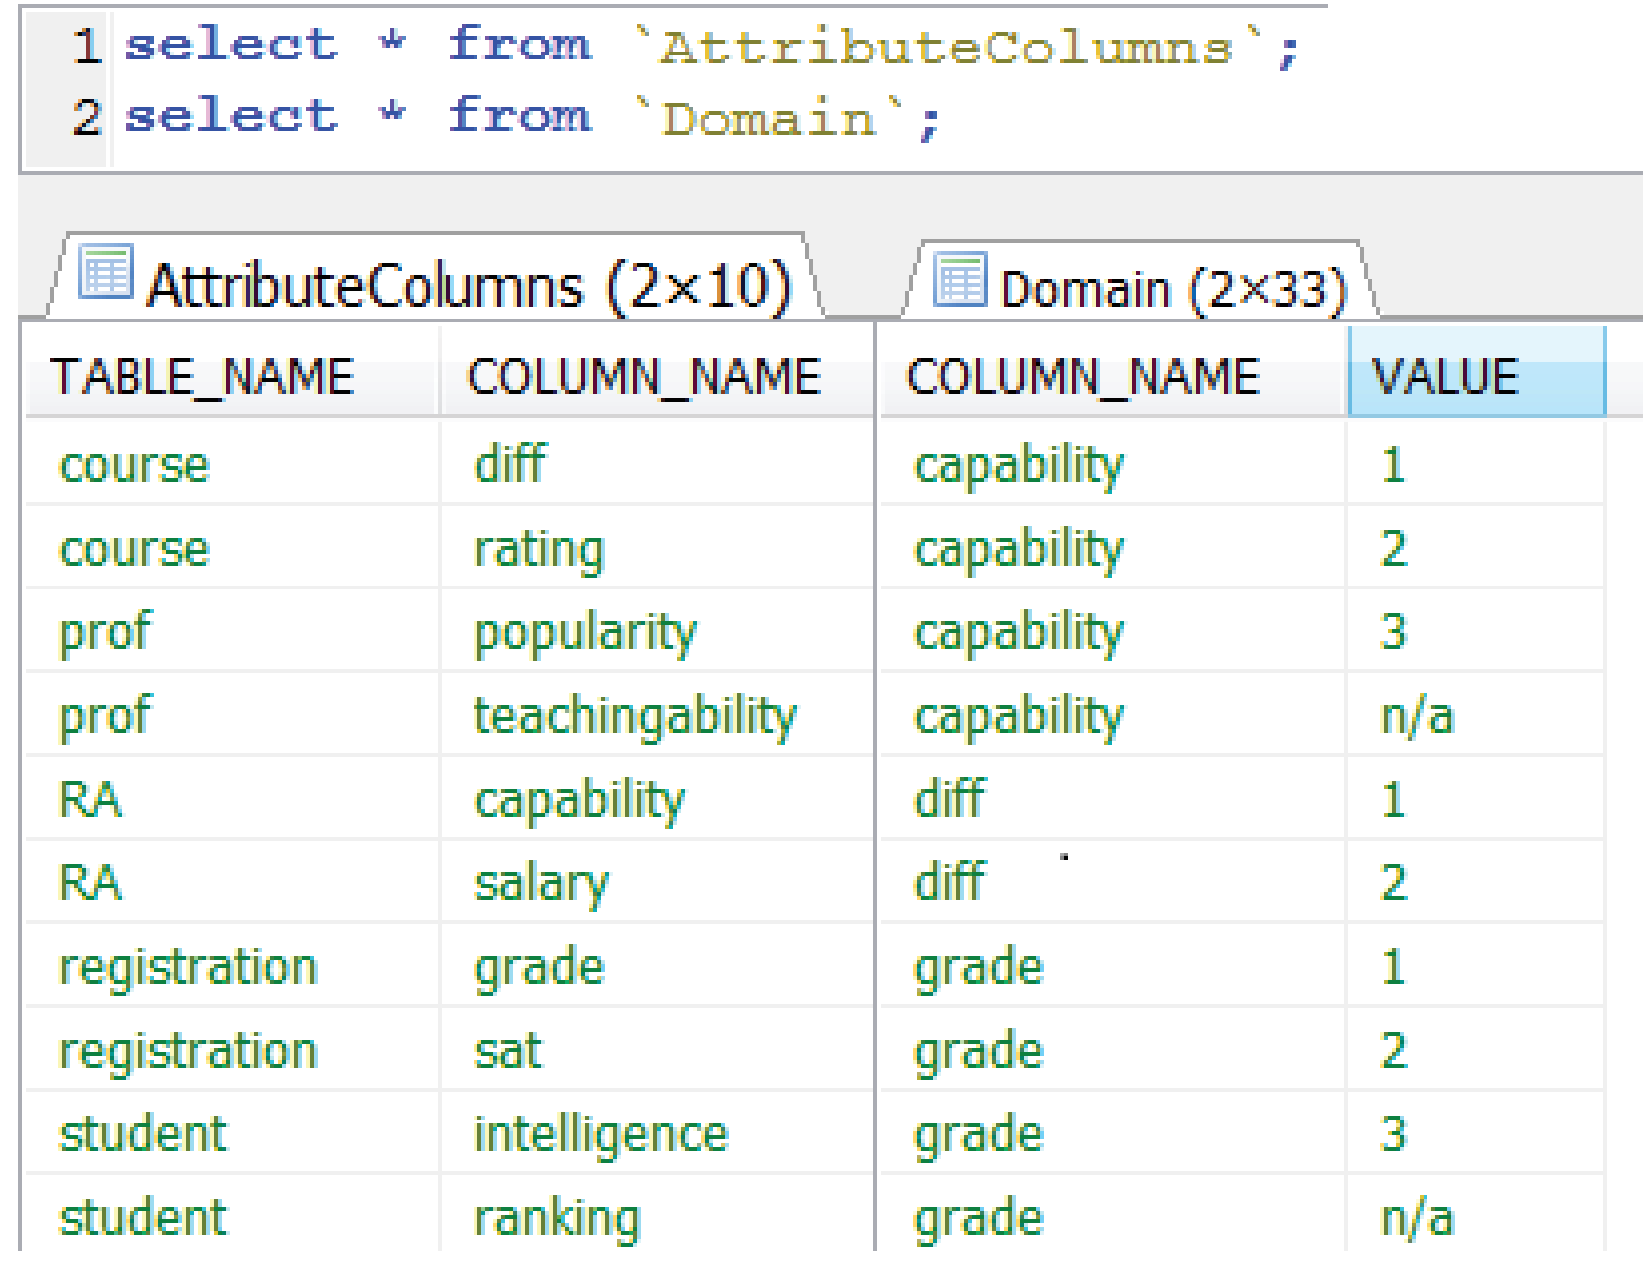
\includegraphics{attribute-domain.pdf} 
} 
\caption{ The metadata about attributes represented in \RVD database tables.  Left: The table $\it{AttributeColumns}$ specifies which tables and columns contain the functor values observed in the data. The column name is also the functor ID. Right: The table $\it{Domain}$ lists the domain for each functor.
}
 \label{fig:attributes}
\end{figure}


 
The metadata must be machine-readable. Following the in-database design philosophy, I  store the metadata in tables so that an SRL algorithm can query it using SQL. The {\em schema analyzer} uses an SQL script that queries key constraints in the system catalog database and {\em automatically} converts them into metadata stored in the random variable database $VDB$. In contrast, existing SRL systems require users to specify information about par-RVs and associated types. 
Thus FactorBase   utilizes the data description resources of SQL to facilitate the ``setup task'' for relational learning \cite{Walker2010}. 
Here, I  illustrate the general principles with the ER diagram of the University domain (Figure~\ref{fig:university-schema}).\footnote{A full description is available~\cite{Schulte2015}.
}



The translation of an ER diagram into a set of functors converts each element of the diagram into a functor, except for entity sets and key fields~\cite{Heckerman+al:SRL07}. Table~\ref{table:translation} illustrates this translation. In terms of database tables, attribute par-RVs correspond to {\em columns}. Relationship par-RVs correspond to {\em tables}, not columns. Including a relationship par-RV in a statistical model allows the model to represent uncertainty about whether or not a relationship exists between two entities~\cite{Kimmig2015}. The values of descriptive attributes of relationships are undefined for entities that are not related. I  represent this by introducing a new constant $\it{n/a}$ in the domain of a relationship attribute~\cite{Milch2005}; see Figure~\ref{fig:attributes} (right). Table~\ref{table:vdb-schema} shows the schema for some of the tables that store metadata for 
each relationship par-RV, as follows. par-RV and FO-Var are custom types.

\begin{description}
\item[Relationship] The associated input data table.
\item[Relationship\_Attributes] Descriptive attributes associated with the relationship and with the entities involved.
\item[Relationship\_FOVariables] The first-order variables contained in each relationship par-RV.\footnote{The schema assumes that all relationships are binary.}
\end{description}


\begin{table}[btp]
\caption{Translation from an ER Diagram to Par-RVs}
 \centering
\resizebox{1\textwidth}{!}{
\begin{tabular}[c]{|l|l|l|}\hline
 ER Diagram &  Example &par-RV equivalent \\\hline
Entity Set  &Student, Course & $\S, \C$ \\\hline
 Relationship Set &RA & RA($\P$,$\S$) \\\hline
Entity Attributes  &intelligence, ranking & Intelligence($\S$), Ranking($\S$) \\\hline
Relationship Attributes  &capability, salary &Capability($\P, \S$), Salary($\P, \S$) \\\hline
\end{tabular}
}
 \label{table:translation}
\end{table}



\begin{table}[hbtp]
\caption{Selected Tables In the Variable Database Schema.}
 \centering
\begin{tabular}{|l|p{10cm}|}
\hline
    {Table Name}&  {Column Names} \\\hline
{Relationship} & {RVarID: par-RV,  TABLE\_NAME: string} \\\hline
    {Relationship\_Attributes}&  {RVarID: par-RV, AVarID: par-RV,  FO-ID: FO-Var} \\\hline
    {Relationship\_FOvariables} & {RVarID: par-RV, FO-ID: FO-Var,  TABLE\_NAME: string}\\\hline
        \end{tabular}%
 \label{table:vdb-schema}
\end{table}


While I  have described constructing the variable database for an ER model, different structured data models can be represented by an appropriate first-order logic vocabulary \cite{Kimmig2015}, that is, an appropriate choice of functors. For example, in a star schema, facts can be represented in the form $\functor(\dimension_{1},\ldots,\dimension_{k})$, where the first-order variable $\dimension_{i}$ ranges over the primary key of dimension table $i$. Attributes of dimension $i$ can be represented by a unary functor $\attribute(\dimension_{i})$. FactorBase can perform structure learning for different data models after the corresponding data format has been translated into the \RVD format.


\section{The Count Manager} \label{sec:count}
The \textbf{count database} \CDB stores a set of  {\em contingency tables}. Contingency tables represent sufficient statistics as follows~\cite{Moore1998, Qian2014a}. 
Consider a fixed list of par-RVs.
A \textbf{query} is a set of $(variable = value)$ pairs where each value is of a valid type for the variable. 
The \textbf{result set} of a query in a database $\D$ is the set of instantiations of the logical variables such that the query evaluates as true in $\D$.
For example, in the database of Figure~\ref{fig:university-tables} the result set for the query 
$\it{RA}(\P,\S) = \true$, $\it{Capability}(\P,\S) = 3$, $\it{Salary}(\P,\S) = \it{high} $ is
the singleton $\{\langle \it{jack}, \it{oliver}\rangle\}$. 
The \textbf{count} of a query is the cardinality of its result set. 

Every set of par-RVs $\set{V} \equiv \{\V_{1},\ldots,\V_{n} \}$ has an associated \textbf{contingency table} ($\cttable$) denoted by $\cttable(\set{V})$.
This is a table with a row for each of the possible assignments of values to the variables in $\set{V}$, and a special integer column called $\qcount$. 
The value of the $\qcount$ column in a row 
corresponding to $V_{1} = v_{1},\ldots,V_{n} = v_{n}$ records the count of the 
corresponding query. 
Figure~\ref{fig:pbn} (b) shows a contingency table for the par-RVs $\it{RA}(\P,\S)$, $\it{Capability}(\P,\S)$, $\it{Salary}(\P,\S)$. 
The value of a relationship attribute is undefined for entities that are not related.
Following \cite{Russell2010}, I  indicate this by writing 
$\it{capability(\P,\S)} = n/a $ for a reserved constant $\it{n/a}$. 
The assertion $\it{capability(\P,\S)}$ = n/a is therefore equivalent to the assertion that $\ra(\P,\S) = \false$. A \textbf{conditional contingency table}, written $$\ct(V_{1},\ldots,V_{k}|V_{k+1} = v_{k+1},\ldots, V_{k+m} = v_{k+m})$$
is the contingency table whose column headers are $V_{1},\ldots,V_{k}$ and whose rows comprise the subset that match the conditions to the right of the $\vert$ symbol.  %  \textbar 
I  assume that contingency tables omit rows with count 0.

The \textbf{contingency table problem} is to compute a contingency table for par-RVs $\set{V} $ and an input database $\D$.  
This is one of the key issues that most of the learning time is taken up. To improve scalability, computing sufficient statistics needs to be feasible for cross product sizes in the millions or more.  I will introduce one Virtual Join method in chapter \ref{cha:multiStatistic}, which is a good solution that computes sufficient statistics without materializing table joins.% \cite{Schulte2012b,Yin2004, Qian2014}.

\section{The Model Manager}\label{sec:mod}
The Model Manager provides two key services for statistical-relational structure learning: 
\begin{enumerate}
\item Estimating and storing parameter values (line 5 of Algorithm~\ref{alg:learning}). 
\item Computing one or more model selection scores (line 7 of Algorithm~\ref{alg:learning}).
\end{enumerate}
 FactorBase  uses a {\em store+score} design for these services, which is illustrated in Figure~\ref{fig:learning}. 
A \textbf{model structure table} represents a candidate model. When a candidate model structure is inserted, a view uses the sufficient statistics from a contingency table to compute a table of parameter values. Another view uses the parameter values and sufficient statistics together to compute the score for the candidate model. In this store+score design, the RDBMS provides model selection scores as a service to the SRL client. 
In many industrial scenarios (e.g. topic modeling: given a large collection of documents, infer the topics contained in each document), one need to deal with very big model containing millions to billions of parameters, the PS paradigm is a very promising approach which could be integrated into the Model Manager \cite{Li2014}.


\begin{figure}[htbp]
\begin{center}
\resizebox{0.8\textwidth}{!}{
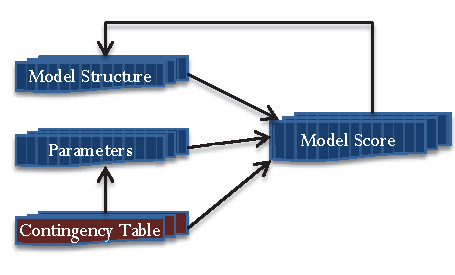
\includegraphics{learning}
}
\caption{Dependencies Among Key Components of the Model  Manager. 
\label{fig:learning}}
\end{center}
\end{figure}

\subsection{The $\MDB$ Schema}
The relational schema for the Models Database is shown in Table~\ref{table:mdb-schema}. The @par-RVID@ parameter refers to the ID  of a par-RV, for instance $\it{Capability}(\P,\S)$.
The model manager stores a set of factor tables (cf. Section~\ref{sec:examples}). In a graphical model, each factor is defined by the local topology of the model template graph. For concreteness, I  illustrate how factor tables can be represented  for Bayesian networks. The graph structure can be stored straightforwardly in a database table $\it{BayesNet}$ whose columns are $\it{child}$ and $\it{parent}$. The table entries are the IDs of par-RVs. An entry such as $(\it{Capability}(\P,\S),\it{Salary}(\P,\S))$ means that $\it{Capability}(\P,\S)$ is a child of $\it{Salary}(\P,\S)$.  For each node, the $\MDB$ manages a conditional probability table. This is a factor table that represents the factor associated with the node's family (see Figure~\ref{fig:ct-cp-table}(b)).

\begin{figure}[!h]
 \centering
\resizebox{0.9\textwidth}{!}{
 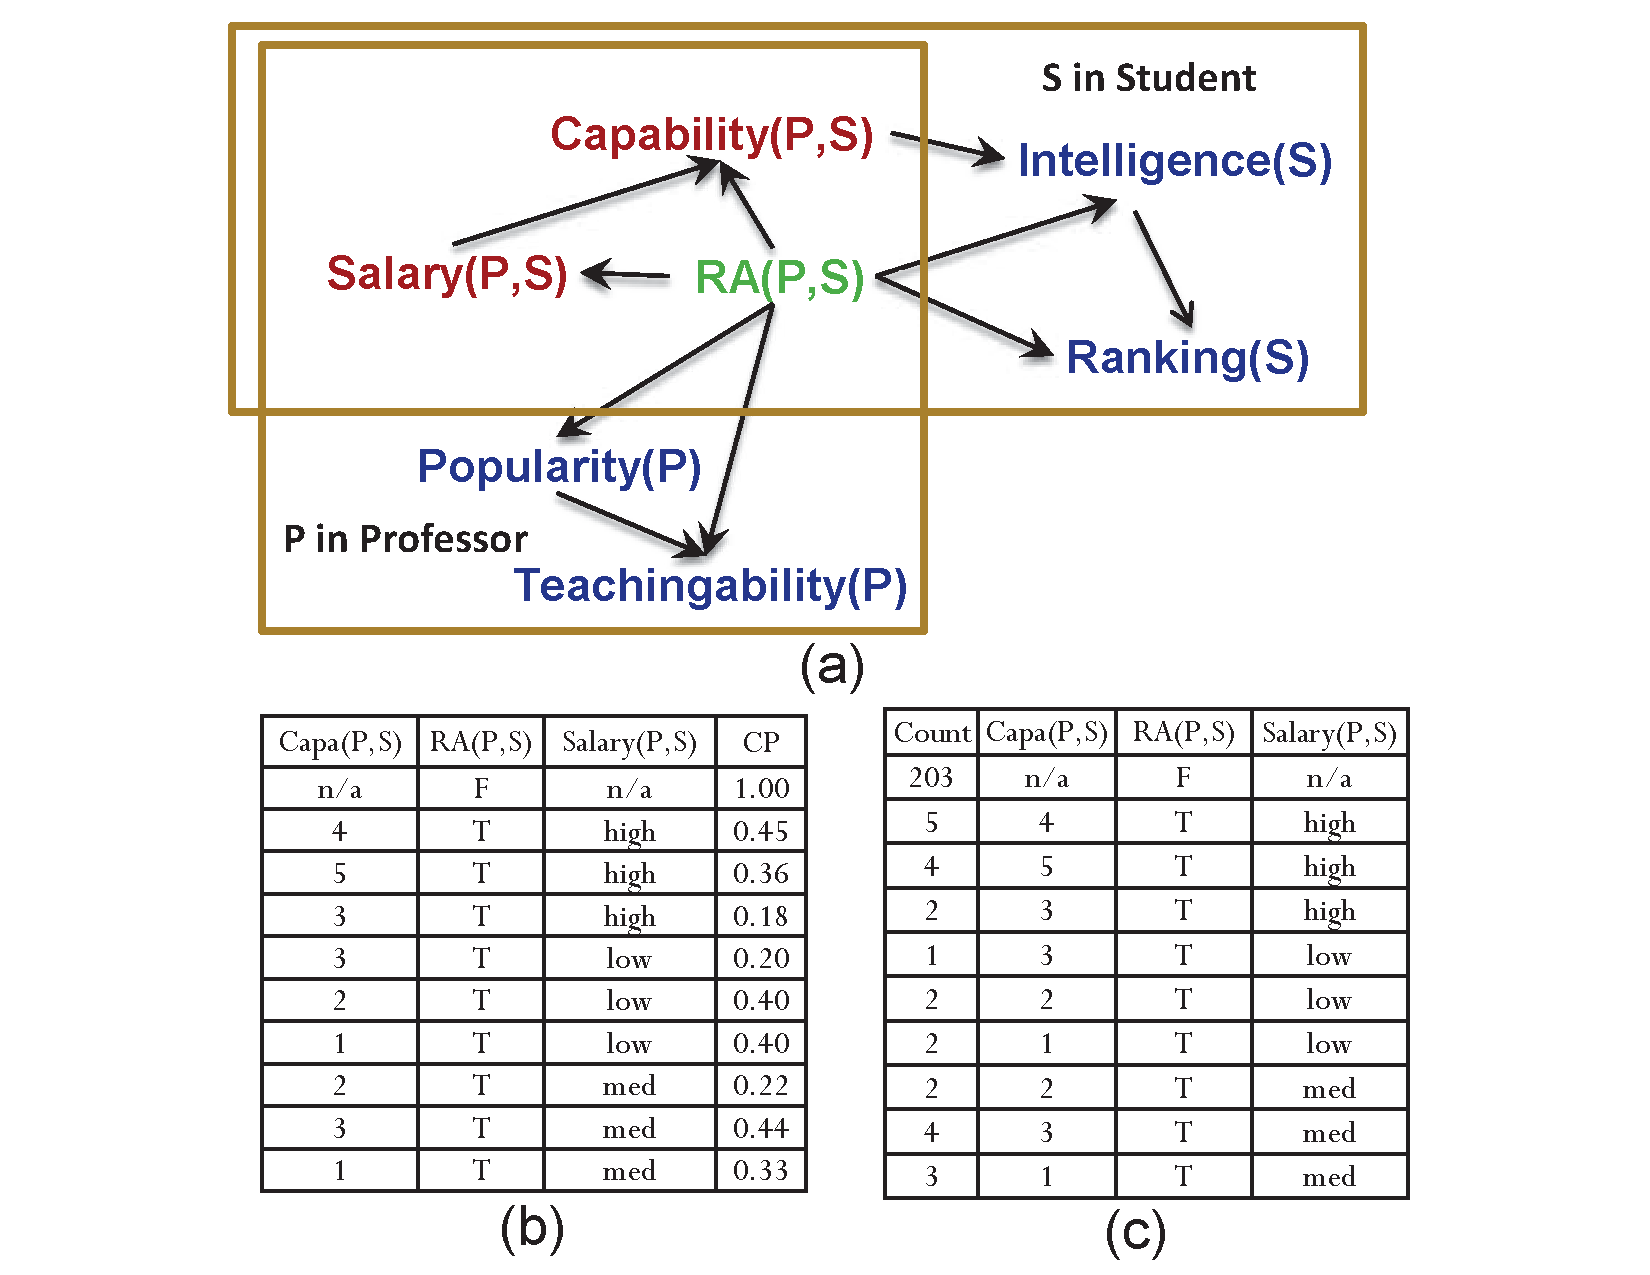
\includegraphics{pbn.pdf} 
} 
\caption{(a) Bayesian network for the University domain. I  omit the $\it{Registered}$ relationship for simplicity. The network was learned from the University dataset \cite{bib:bbsite}. (b) Conditional Probability table $Capability(\P,\S)\_\cptable$, for the node $Capability(\P,\S)$. Only value combinations that occur in the data are shown. This is an example of a factor table. (c) Contingency Table $Capability(\P,\S)\_\cttable$ for the node $Capability(\P,\S)$ and its parents. Both CP and CT tables are stored in an RDBMS.}
\label{fig:ct-cp-table}
\end{figure}
In a Bayesian network, model selection scores are decomposable. This means that there is a local score associated with each family, such that the total score for the BN model is the sum of the local scores. For each family, the local score is stored in the $\it{Scores}$ table indexed by the family's child node.
%These $\cpt$s are also stored in the Models Database $\MDB$. 


%3) Inferring a model prediction for a set of test instances and scoring the model against the true values. 
%I  also discuss model structure learning. 


\subsection{Parameter Manager} \label{sec:parameters}
Deriving predictions from a model requires estimating values for its parameters.  Maximizing the data likelihood is the basic parameter estimation method for Bayesian networks. The maximum likelihood estimates equal the observed frequency of a child value given its parent values.
% \cite{Schulte2012}. 


\begin{table}[!h]
\caption{The main tables in the Models Database $\MDB$. For a Bayesian network, the $\MDB$ stores its structure, parameter estimates, and model selection scores.}
 \centering
 \begin{tabular}
[c]{|l|}\hline
BayesNet(\underline{child:par-RV,parent:par-RV})\\
@par-RVID@\_CPT(\underline{@par-RVID@:par-RV,$\mbox{parent}_{1}$:par-RV,$\ldots,\mbox{parent}_{k}$:par-RV},cp:real)\\ 
Scores(\underline{child:par-RV},loglikelihood:real,\#par:int,aic:real)\\
\hline
\end{tabular}
 %\textbf{Oliver:based on the template: caption of table should be above the table?}
\label{table:mdb-schema}
\end{table}
%\paragraph{SQL Construction of Conditional Probability Tables} 
{\em SQL Implementation of Conditional Probability Tables With Natural Join.} Given the sufficient statistics in a contingency table, a conditional probability table containing the maximum likelihood estimates can be computed by aggregation using SQL.  As shown in Figure~\ref{fig:ct-cp-table}(b)\footnote{Same as Figure \ref{fig:pbn}.}, the conditional probability table $Capability(\P,\S)\_\cptable$, for the node $Capability(\P,\S)$ is computed as below. 
%Only value combinations that occur in the data are shown. 
\begin{alltt}
SELECT count/temp.parent\_count as CP, 
capability(P,S), RA(P,S), salary(P,S) 
FROM capability(P,S)\_CT 
	NATURAL JOIN  
(SELECT sum(Count) as parent\_count, 
RA(P,S), salary(P,S) 
FROM capability(P,S)\_CT  
GROUP BY  RA(P,S), salary(P,S) ) as temp
\end{alltt}



\subsection{Model Score Computation} \label{sec:model-score}
A typical model selection approach is to maximize the likelihood of the data, balanced by a penalty term. For instance, the Akaike Information Criterion (AIC) is defined as follows 
\[\mathit{AIC}(\G,\D) \equiv ln(P_{\widehat{G}}(\D)) - \parameters(\G) \]
where $\widehat{G}$ is the BN $\G$ with its parameters instantiated to be the maximum likelihood estimates given the database $\D$, and $\parameters(\G)$ is the number of free parameters in the structure $\G$. 
The number of free parameters for a node is the product of (the possible values for the parent nodes) $\times$ (the number of the possible values for the child node -1). Given the likelihood and the number of parameters, the AIC column is computed as $\aic = \loglikelihood - \parameters$. 
 Model selection scores other than AIC can be computed in a similar way given the model likelihood and number of parameters.

\paragraph{Parameter Number Computation} To determine the number of parameters of the child node @parVar-ID@, the number of possible child and parent values can be found from the $\it{\RVD.Domain}$ table in the Random Variable Database.  

\paragraph{Likelihood Computation} As explained in Section~\ref{sec:log-linear}, the log-likelihood can be computed by multiplying the instantiation counts of a factor by its value. Assuming that instantiation counts are represented in a contingency table and factor values in a factor table, this multiplication can be elegantly performed using the Natural Join operator. For instance, the log-likelihood score associated with the $Capability(\P,\S)$ family is given by the SQL query below.

\begin{alltt}
SELECT Capability(P,S),  SUM(CPT.cp * CT.count) AS loglikelihood
FROM MDB.Capability(P,S)\_CPT as CPT
NATURAL JOIN CDB.Capability(P,S)\_CT as CT
\end{alltt}

The aggregate computation in this short query illustrates how well SQL constructs support complex computations with structured objects. This completes the description of how the modules of FactorBase  are implemented using SQL. I  next show how these modules support a key learning task: computing the predictions of an SRL model on a test instance. 


\section{Test Set Predictions} Computing probabilities over the label of a test instance is important for several tasks. 
\begin{enumerate}
\item Classifying the test instance, which is one of the main applications of a machine learning system for end users.
\item Comparing the class labels predicted against true class labels is a key step in several approaches to model scoring \cite{Kimmig2015}. 
\item Evaluating the accuracy of a machine learning algorithm by the train-and-test paradigm, where the system is provided a training set for learning and then one test its predictions on unseen test cases. 
\end{enumerate}

I  first discuss how to compute a prediction for a single test case, then how to compute an overall prediction score for a set of test cases. 
Recall that log-linear equation \ref{eq:parfactor} is as follows \cite[Eq.7]{Kimmig2015}:
\begin{equation} \nonumber
P(\set{X}=\set{x}) = \frac{1}{Z} \prod_{\parfactor_{i} \in \parfactors} \prod_{\gparrvs \in \instantiations(\parfactor_{i})} 
\potential_{i}(\set{x}_{\gparrvs}) 
\end{equation}
where $\set{x}_{\gparrvs}$ represents the values of those variables in $\gparrvs$ that are necessary to compute $\potential_{i}$. 

Class probabilities can be derived from above Equation as follows.
Let $\Y$ denote a ground par-RV to be classified, which I  refer to as the \textbf{target variable}. For example, a ground atom may be $\it{Intelligence}(jack)$. In this example, I  refer to jack as the \textbf{target entity}. Write $\set{X}_{-\Y}$ for a database instance that specifies the values of all ground par-RVs, except for the target, which are used to predict the target node. Let $[\set{X}_{-\Y},\y]$ denote the completed database instance where the target node is assigned value $\y$. The log-linear model uses the likelihood $P([\set{X}_{-\Y},\y])$ as the joint score of the label and the predictive features. The conditional probability is proportional to this score:
\begin{equation} \label{eq:classify}
P(\y|\set{X_{-\Y}}) \propto P([\set{X}_{-\Y},\y])
\end{equation}
where the joint distribution on the right-hand side is defined by Equation~\ref{eq:parfactor}, and the scores of the possible class labels need to be normalized to define  conditional probabilities. 


\begin{table*}[!h]
\caption{SQL queries for computing target contingency tables supporting test set prediction.  $\textless$Attribute-List$\textgreater$ and  $\textless$Key-Equality-List$\textgreater$ are as in Figure~\ref{fig:meta-query}.}
\begin{center}
\begin{tabular}{|c|p{5cm}|p{4cm}|p{3cm}}
Access &SELECT&WHERE&GROUP BY\\\hline
Single &COUNT(*) AS count, $\textless$Attribute-List$\textgreater$, S.sid& $\textless$Key-Equality-List$\textgreater$ AND S.s\_id = jack&  $\textless$Attribute-List$\textgreater$\\
\hline
Block & COUNT(*) AS count,  $\textless$Attribute-List$\textgreater$, S.sid& $\textless$Key-Equality-List$\textgreater$ &  $\textless$Attribute-List$\textgreater$, \textbf{S.sid}\\
\end{tabular}
\end{center}
\label{table:target-query}
\end{table*}%

{\em SQL Implementation of the Log-Linear Classification Score} 
The obvious approach to computing the log-linear score would be to use the likelihood computation of Section~\ref{sec:model-score} for the entire database.
%to find the score $P_{G}(\set{X}_{-\Y,\y})$, then normalize. 
This is inefficient because only instance counts that involve the target entity change the classification probability. 
For example, if jack is the target entity, then the grades of jill do not matter. 
This means that I  need only consider query instantiations that match the appropriate logical variable with the target entity (e.g., $\S = jack$). 
I  show how the log-likelihood computation of Section~\ref{sec:model-score} can be adapted to compute a log-linear classification score for a set of target entities. This illustrates how the modularity of FactorBase  supports reusing its components for different tasks. 

For a given set of random variables, target entity instantiation counts can be represented in a contingency table that I  call the \textbf{target contingency table}. Figure~\ref{fig:targetct} shows the format of a contingency table for target entities Jack resp. Jill.


\begin{figure}[!h] 
 \centering
\resizebox{0.8\textwidth}{!}{
 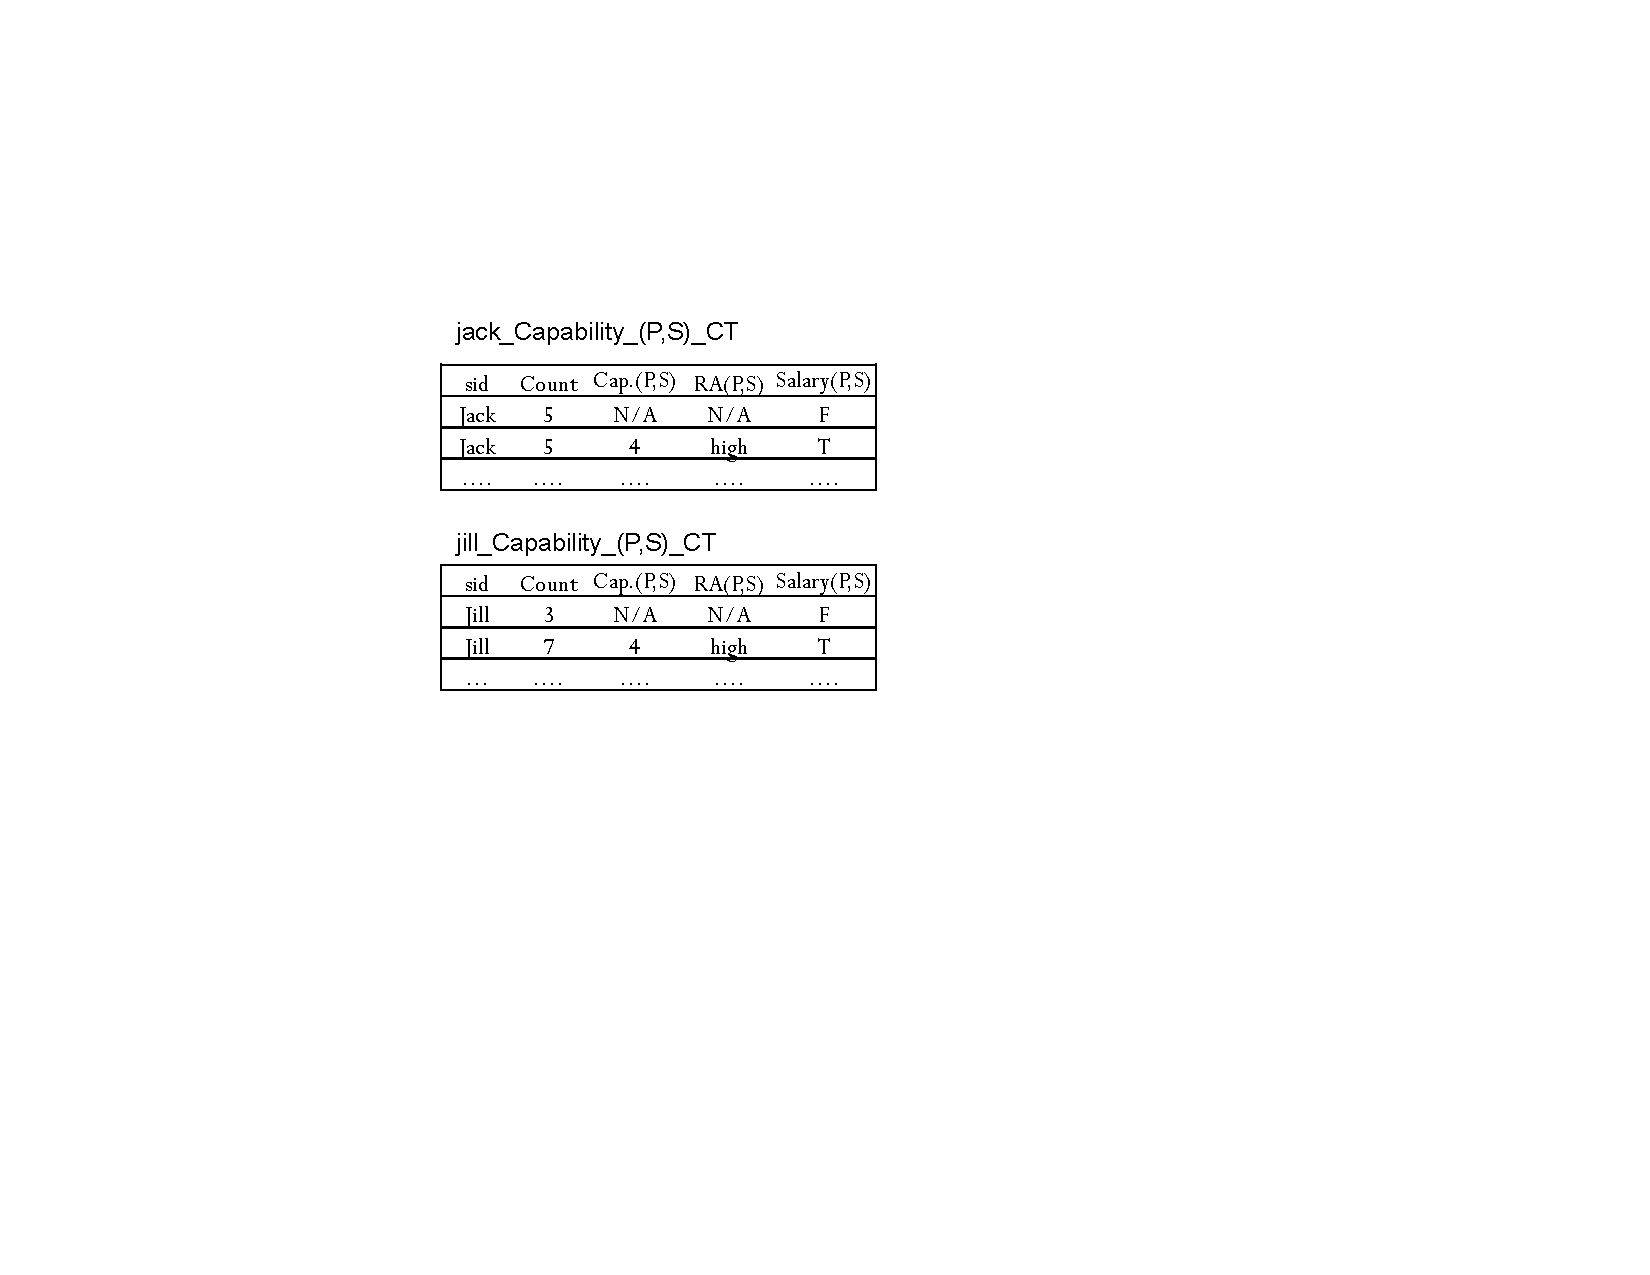
\includegraphics{targetct} 
} 
\caption{Target contingency tables for target = Jack and for target = Jill.}
 \label{fig:targetct}
\end{figure}

{\em Assuming} that for each node with ID @parRVID@, a target contingency table named $\CDB.target\_@\it{parRVID}@\_\cttable$ has been built in the Count Database $\CDB$, the log-likelihood SQL is as in Section~\ref{sec:model-score}. For instance, the contribution of the $Capability(\P,\S)$ family is computed by the SQL query shown,  but with the contingency table jack\_Capability(P,S)\_CT in place of Capability(P,S)\_CT.
The new problem is finding the target contingency table. SQL allows us to solve this easily by restricting counts to the target entity in the WHERE clause. To illustrate, suppose I  want to modify the contingency table query of Figure~\ref{fig:meta-query} to compute the contingency table for $\S = jack$. I  add the student id to the SELECT clause, and the join condition $S.s\_id = jack$ to the WHERE clause; see Table~\ref{table:target-query}.\footnote{Omit apostrophes for readability.} 
The FROM clause is the same as in Figure~\ref{fig:meta-query}. The metaquery of Figure~\ref{fig:meta-query} is easily changed to produce these SELECT and WHERE clauses. The details of metequery will be discussed in section \ref{sub:meta}.

Next consider a setting where a model is to be scored against an entire test set. This occurs for instance in the standard cross-validation computation for model scoring. For concreteness, suppose the problem is to predict the intelligence of a set of students
 $\it{Intelligence}(jack)$, $\it{Intelligence}(jill)$, $\it{Intelligence}(student_{3}),\ldots, \it{Intelligence}(student_{m})$.
An obvious approach is to loop through the set of test instances, repeating the likelihood query above for each single instance. Instead,  SQL supports {\em block access} where I  process the test instances as a block. Intuitively, instead of building a contingency table for each test instance, I  build a single contingency table that stacks together the individual contingency tables (Figure~\ref{fig:targetct}). Blocked access can be implemented in a beautifully simple manner in SQL: I  simply add the primary key id field for the target entity to the GROUP BY list; see Table~\ref{table:target-query}. 

\section{Evaluation} 
The experimental study describes how FactorBase  can be used to implement a challenging machine learning application: Constructing a Bayesian network model for a relational database. Bayesian networks are a good illustration of typical challenges and how RDBMS capabilities can address them. I will explain the learning details in chapter \ref{cha:lbn}. 
In the experiments I  followed a {\em pre-counting} approach where the count manager constructs a \textbf{joint contingency table} for {\em all} par-RVs in the random variable database. 


Code was written in MySQL Script and Java, JRE 1.7.0.  and executed with 8GB of RAM and a single Intel Core 2 QUAD Processor Q6700 with a clock speed of 2.66GHz (no hyper-threading). The operating system was Linux Centos 2.6.32.  The MySQL Server version 5.5.34 was run with 8GB of RAM and a single core processor of 2.2GHz.  All code and datasets are available on-line \cite{bib:bbsite}. 


\subsection{Datasets} \label{sec:datasets}
I  used six benchmark real-world databases. For detailed descriptions and  the sources of the databases, please see \cite{bib:bbsite} and the references therein. Table~\ref{table:datasets} summarizes basic information about the benchmark datasets.  
IMDb is the largest dataset in terms of number of total tuples (more than 1.3M tuples) and schema complexity. %attributes.
It combines the MovieLens database\footnote{www.grouplens.org, 1M version} with data from the Internet Movie Database (IMDb)\footnote{www.imdb.com, July 2013} following \cite{Peralta2007}. Table~\ref{table:datasets} provides information about the number of par-RVs generated for each database. More complex schemas 
%and self-relationships 
generate more random variables. 


\begin{table}[!h] 
\caption{Datasets characteristics. 
\\ \#Tuples = total number of tuples over all tables in the dataset. \label{table:datasets}}
 \centering
%\scalebox{0.7in}{
\resizebox{0.9\textwidth}{!}{
\begin{tabular}[c]
{|l|c|c|r|c|}\hline
 \textbf{Dataset} & \textbf{\begin{tabular}[l] {ll} \#Relationship \\Tables/ Total \end {tabular}} & \textbf{\begin{tabular}[l] {ll} \# par-RV \end {tabular}}  & \textbf{\#Tuples} 
%& \textbf{\#Attributes}  
\\\hline
% \textbf{Dataset} & \textbf{Relationships} & \textbf{\begin{tabular}[l] {ll} Self \\Relationships \end {tabular}} &
% \textbf{\begin{tabular}[l] {ll} Same Type\\ Relationships \end {tabular}}& \textbf{\#Tuples} & \textbf{\begin{tabular}[l] {ll} \#Attribute  \\Columns \end{tabular}}  \\\hline
 %   University&2 & 0 & N & 171 & 12\\\hline
    Movielens &1 / 3 & 7  & 1,010,051 
%& 7
\\\hline
%    Movielens(0.1M) &1 & N & N &  83,402 & 7\\\hline
    Mutagenesis & 2 / 4 & 11 & 14,540 
%& 11
\\\hline
 UW-CSE &2 / 4 & 14  & 712 %& 14
\\\hline   
  Mondial &2 / 4 & 18 &  870
%& 18
\\\hline
    %Financial &3 / 7 & 0  &  225,932& 15\\\hline
   Hepatitis &3 / 7 & 19 &12,927  
%& 19
\\\hline
   IMDb &3 / 7 & 17 &1,354,134  %& 17
\\\hline   
\end{tabular}
}
\end{table}


%


\subsection{Results}
Table~\ref{tab:counts} reports the number of sufficient statistics for constructing the joint contingency table. This number depends mainly on the number of par-RVs. The number of sufficient statistics can be quite large, over 15M for the largest dataset IMDb.  Even with such large numbers, constructing contingency tables using the SQL metaqueries is feasible, taking just over 2 hours for the very large IMDb set. 
The number of Bayesian network parameters is much smaller than the number of sufficient statistics. The difference between the number of parameters and the number of sufficient statistics measures how compactly the BN summarizes the statistical information in the data. 


\begin{table}[!h]
  \caption{Count Manager: Sufficient Statistics and Parameters}
  \centering
   \resizebox{0.9\textwidth}{!}{ \begin{tabular}{|l|r|r|r|r|r|}
    \hline
 \textbf{  Dataset  }&  \textbf{ \begin{tabular}[l] {ll} \# Database\\Tuples  \end{tabular} }&\textbf{ \begin{tabular}[l] {ll}\# Sufficient \\ Statistics (SS) \end{tabular}}& \textbf{\begin{tabular}[l] {ll} SS \\Computing\\ Time (s) \end{tabular}} &\textbf{\begin{tabular}[l] {ll}  \#BN \\ Parameters  \end{tabular}}%& \textbf{\begin{tabular}[l] {ll}Para. \\Learning\\ Time (s) \end{tabular} }
\\
    \hline
    Movielens & 1,010,051 & 252   & 2.7   & 292   \\%& 0.57  \\
    \hline
    Mutagenesis & 14,540 & 1,631 & 1.67  & 721   \\%& 0.98  \\
    \hline
    UW-CSE & 712   & 2,828 & 3.84  & 241   \\%& 1.14  \\
    \hline
    Mondial & 870   & 1,746,870 & 1,112.84 & 339  \\% & 60.55  \\
    \hline
%    Financial & 225,932 & 3,013,011 & 1,421.87 & 2,433  & 88.974  \\
%    \hline
    Hepatitis & 12,927 & 12,374,892 & 3,536.76 & 569   \\%& 429.15  \\
    \hline
    IMDb  & 1,354,134 & 15,538,430 & 7,467.85 & 60,059 \\%& 505.61  \\
    \hline
    \end{tabular}%
}
 \label{tab:counts}
\end{table}%


 
Table~\ref{tab:counts} shows that Bayesian networks provide very compact summaries of the data statistics. For instance for the Hepatitis dataset, the ratio is  $12,374,892/569 > 20,000$. The IMDb database is an outlier, with a complex correlation pattern that leads to a dense Bayesian network structure.

Table~\ref{tab:model} shows that the graph structure of a Bayesian network contains a small number of edges relative to the number of parameters. 
The parameter manager provides fast maximum likelihood estimates for a given structure. 
This is because computing a local contingency table for a BN family is fast given the joint contingency table.
%

\begin{table}[!h]
\caption{Model Manager Evaluation}
  \centering
      \resizebox{0.9\textwidth}{!}{ \begin{tabular}{|l|r|r|r|r|}
    \hline
     \textbf{ Dataset} %&  \textbf{ \begin{tabular}[l] {ll}\# Tuples In \\  RRVD \end{tabular} } 
&  \textbf{ \begin{tabular}[l] {ll} \# Edges in \\Bayes Net  \end{tabular} }& \textbf{ \begin{tabular}[l] {ll} \# Bayes Net \\ Parameters   \end{tabular} } & \textbf{\begin{tabular}[l] {ll}Parameter \\Learning\\ Time (s) \end{tabular} }\\
    \hline
    Movielens &   72    %& 12
    & 292 & 0.57  \\
    \hline
    Mutagenesis &   124   % & 57
    & 721 & 0.98  \\
    \hline
    UW-CSE &       112 %& 118
   & 241  & 1.14 \\
    \hline
    Mondial &       141 %& 126 
  & 339 & 60.55    \\
    \hline
    Hepatitis &       207%& 142 
  & 569  & 429.15   \\
    \hline
    IMDb  &      195 %& 217  
 & 60,059   & 505.61\\
    \hline
    \end{tabular}%
}  
  \label{tab:model}%
\end{table}%

Figure~\ref{fig:test-timing} compares computing predictions on a test set using an instance-by-instance loop, with a separate SQL query for each instance, v.s. a single SQL query for all test instances as a block (Table~\ref{table:target-query}). 


\begin{figure}[h] %  figure placement: here, top, bottom, or page
 \centering
\resizebox{0.9\textwidth}{!}{
 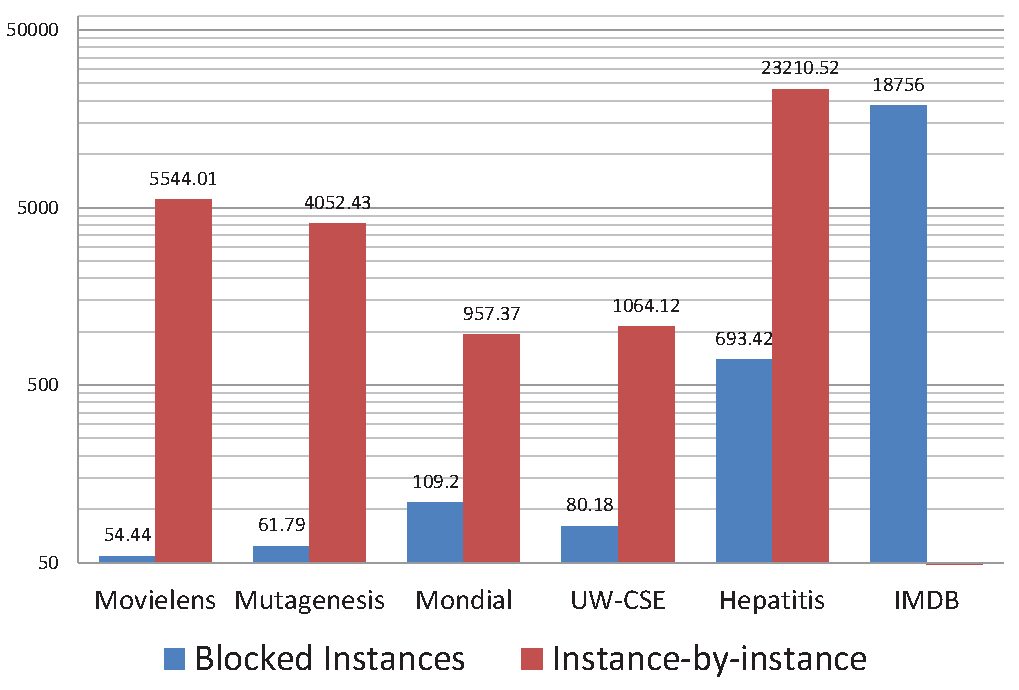
\includegraphics{test-timing.pdf} 
} 
\caption{Times (s) for Computing Predictions on Test Instances. The right red column shows the time for looping over single instances using the Single Access Query of Table~\ref{table:target-query}. The left blue column shows the time for the Blocked Access Query of Table~\ref{table:target-query}.
}
 \label{fig:test-timing}
\end{figure}



\begin{table}[!h]
\caption{\# of Test Instances }
  \centering
  \begin{tabular}{|r|r|r|r|r|r|r|} \hline
\textbf{Dataset}&Movielens&	Mutagenesis	& 	UW-CSE	&	Mondial&	Hepatitis&	 	IMDb \\ \hline
{\#instance}	&4,742	 	&	3,119		&576	&		505&2,376	 	&46,275 \\ \hline
    
\end{tabular}%  
  \label{tab:test-instance}%
\end{table}%
Table \ref{tab:test-instance} specifies the number of  test instances for each dataset. I  split each benchmark database into  80\% training data, 20\% test data. The test instances are the ground atoms of all descriptive attributes of entities.  The blocked access method is 10-100 faster depending on the dataset. The single access method did not scale to the large IMDb dataset (timeout after 12 hours).


\begin{table}[!h] \caption{Learning Time Comparison (sec) with other statistical-relational learning systems. NT = non-termination}
  \centering
      \resizebox{0.9\textwidth}{!}{
\begin{tabular}{|l|r|r|r|r|}\hline
Dataset  & RDN\_Boost  & MLN\_Boost  & FB-Total & FB-Count \\\hline
MovieLens & 5,562  & N/T & 1.12 & 0.39 \\\hline
Mutagenesis  & 118 & 49 & 1 & 0.15 \\\hline
UW-CSE & 15 & 19 & 1 & 0.27 \\\hline
Mondial  & 27 & 42 & 102 & 61.82 \\\hline
Hepatitis  & 251 & 230 & 286 & 186.15 \\\hline
IMDb & N/T & N/T & 524.25 & 439.29 \\\hline
\end{tabular}
} 
  \label{tab:othersrl}%
\end{table}%

Table~\ref{tab:othersrl} reports result for the complete learning of a Bayesian network, structure and parameters. It benchmarks FactorBase against functional gradient boosting, a state-of-the-art  multi-relational learning approach~\cite{Natarajan2012}. 
MLN\_Boost learns a Markov Logic Network, and RDN\_Boost a Relational Dependency Network. I  used the Boostr implementation \cite{Khot2013}. To make the results easier to compare across databases and systems, I  divide the total running time by the number of par-RVs for the database (Table~\ref{table:datasets}). 


Table~\ref{tab:othersrl} shows that structure learning with FactorBase is fast: even the large complex database IMDb requires only around 8 minutes/par-RV. Compared to the boosting methods, FactorBase  shows excellent scalability: neither boosting method terminates on the IMDb database, and while RDN\_Boost terminates on the MovieLens database, it is almost 5,000 times slower than {\sc FactorBase}. 
Much of the speed of my implementation is due to quick access to sufficient statistics. As the last column of Table~\ref{tab:othersrl} shows, on the larger datasets FactorBase spends about 80\% of computation time on gathering sufficient statistics via the count manager. This suggests that a large  speedup for the boosting algorithms could be achieved if they used the FactorBase  in-database design. 

I  do not report accuracy results because predictive accuracy is not the focus of this chapter. 
On the standard conditional log-likelihood metric, as defined by Equation~\ref{eq:classify}, the model learned by FactorBase  performs better than the boosting methods on all databases. This is consistent with the results of previous studies \cite{Schulte2012}. FactorBase  leverages RDBMS capabilities for scalable management of statistical analysis objects. It efficiently constructs and stores large numbers of sufficient statistics and parameter estimates. 
%MRLBase can integrate information from different statistical objects when they are maintained as first-class citizens in the RDBMS. 
The RDBMS support for statistical-relational learning translates into orders of magnitude improvements in speed and scalability.
% compared to other state-of-the-art methods.

%add here




\section{Conclusion} 
Compared to traditional learning with a single data table, learning for multi-relational data requires new system capabilities. In this chapter I  described FactorBase, a system that leverages the existing capabilities of an SQL-based RDBMS to support statistical-relational learning. Representational tasks include specifying metadata about structured first-order random variables, and storing the structure of a learned model. Computational tasks include storing and constructing sufficient statistics, and computing parameter estimates and model selection scores. 
I showed that SQL scripts can be used to implement these capabilities, with multiple advantages. These advantages include: 1) Fast program development through high-level SQL constructs for complex table and count operations. 2) Managing large and complex statistical objects that are too big to fit in main memory.  For instance, some of the benchmark databases require storing and querying millions of sufficient statistics. 

Empirical evaluation on six benchmark databases showed significant scalability advantages from utilizing the RDBMS capabilities: Both structure and parameter learning scaled well to millions of data records, beyond what previous multi-relational learning systems can achieve. 




\chapter{Computing Multi-Relational Sufficient Statistics for Large Databases}\label{cha:multiStatistic}




Relational databases contain information about attributes of entities, and which relationships do and do not hold among entities. To make this information accessible for knowledge discovery  requires computing {\em sufficient statistics}. 
Whereas sufficient statistics with positive relationships only can be efficiently computed by SQL joins of existing database tables, a table join approach is not feasible for negative relationships. Negative relationships concern the nonexistence of a relationship. This is because people would have to enumerate all tuples of entities that are {\em not} related (consider the number of user pairs who are {\em not} friends on Facebook). The cost of the enumeration approach is close to materializing the Cartesian cross product of entity sets, which grows exponentially with the number of entity sets involved. It may therefore seem that sufficient statistics with negative relationships can be computed only for small databases. 

Within this chapter, I describes a new dynamic programming algorithm for computing cross-table sufficient statistics that may contain any number of {\em positive and negative} relationships. I  show that on the contrary, assuming that sufficient statistics with positive relationships are available, extending them to negative relationships can be achieved in a highly scalable manner, which does not depend on the size of the database.
\section{Introduction} 

\subsection{Virtual Join Approach} My approach to this problem introduces a new Virtual Join operation. A Virtual Join algorithm computes sufficient statistics {\em without} materializing a cross product \cite{Yin2004}. Sufficient statistics can be represented in contingency tables \cite{Moore1998}. The Virtual Join operation is a dynamic programming algorithm that successively builds up a large contingency table from smaller ones, {\em without a need to access the original data tables}. I  refer to it as the M\"obius Join since it is based on the M\"obius extension theorem \cite{Schulte2014}.

I  introduce algebraic operations on contingency tables that generalize standard relational algebra operators. I  establish a contingency table algebraic identity that reduces the computation of sufficient statistics with $k+1$ negative relationships to the computation of sufficient statistics with only $k$ negative relationships. 
The M\"obius Join applies the identity to construct contingency tables that involve $1,2,\ldots,\ell$ relationships (positive and negative), until I  obtain a joint contingency table for all tables in the database. A theoretical upper bound for the number of contingency table operations required by the algorithm is $O(r \log r)$,  where $r$ is the number of sufficient statistics involving negative relationships. In other words, the number of table operations is nearly linear in the size of the required output. 

\subsection{Evaluation} I  evaluate the {\em scalability} of my M\"obius Join algorithm by computing contingency tables for seven real-world databases. The observed computation times exhibit the near-linear growth predicted by the theoretical analysis. They range from two seconds on the simpler database schemas to just over two hours for the most complex schema with over 1 million tuples from the IMDb database.

Given that computing sufficient statistics for negative relationships is {\em feasible}, the remainder of the experiments evaluate their {\em usefulness}. These sufficient statistics allow statistical analysis to utilize the absence or presence of a relationship as a feature. 
The benchmark datasets provide evidence that the positive and negative relationship features enhance different types of statistical analysis, as follows. 
\begin{enumerate}
\item Feature selection: When provided with sufficient statistics for negative and positive relationships, a standard feature selection method selects relationship features for classification.
\item Association Rule Mining: A standard association rule learning method includes many association rules with relationship conditions in its top 20 list. 
\end{enumerate}


\paragraph{ Contributions} My main contributions are as follows.
\begin{enumerate}
\item A dynamic program to compute a joint contingency table for sufficient statistics that combine several tables, and that may involve any number of {\em positive and negative }relationships.
\item An extension of relational algebra for contingency tables that supports the dynamic program conceptually and computationally.
\end{enumerate}


\emph{Chapter Organization} 
The main part of the chapter describes the dynamic programming algorithm for computing a joint contingency table for all random variables. I  define the contingency table algebra.  A complexity analysis establishes feasible upper bounds on the number of contingency table operations required by the M\"obius Join algorithm. I  also investigate the scalability of the algorithm empirically. The final set of experiments examines how the cached sufficient statistics support the analysis of cross-table dependencies for different learning and data mining tasks.


 
\section{Background and Notation} \label{sec:variables}

As described in section \ref{chaSecRVD}, I  assume a standard \textbf{relational schema} containing a set of tables, each with key fields, descriptive attributes, and possibly foreign key pointers. A \textbf{database instance} specifies the tuples contained in the tables of a given database schema, see Figure \ref{fig:university-schema} and \ref{fig:university-tables}. I  also adopt the function-based notation from section \ref{chaSecRVD}. 

The functor formalism is rich enough to represent the constraints of an entity-relationship schema via the following translation: Entity sets correspond to populations, descriptive attributes to functions, relationship tables to relationships, and foreign key constraints to type constraints on the arguments of relationship predicates. Table~\ref{table:translation}  illustrates this translation, distinguishing attributes of entities ($\eatts$) and attributes of relationships ($\ratts$). 

\subsection{Related Work} 

\paragraph{Sufficient Statistics for Single Data Tables} Several data structures have been proposed for storing sufficient statistics defined on a {\em single} data table.  One of the best-known are ADtrees \cite{Moore1998}.  An ADtree provides a memory-efficient data structure for {\em storing} and retrieving sufficient statistics once they have been computed. In this chapter, I focus on the problem of {\em computing} the sufficient statistics, especially for the case where the relevant rows have not been materialized. Thus ADtrees and contingency tables are complementary representations for different purposes: contingency tables support a computationally efficient block access to sufficient statistics, whereas ADtrees provide a memory efficient compression of the sufficient statistics.  An interesting direction for future work is to build an ADtree for the contingency table once it has been computed. 

\paragraph{Relational Sufficient Statistics} 
Schulte {\em et al.} review previous methods for computing statistics with negative relationships \cite{Schulte2014}. They show that the fast M\"obius transform can be used in the case of multiple negative relationships. Their evaluation considered only Bayes net parameter learning with only one relationship. I  examined computing joint sufficient statistics over the entire database.  Other novel aspects are the $\ct$-table operations and using the relationship chain lattice to facilitate dynamic programming. 



\subsection{Review of Contingency Table}

Here I review the {\em contingency table}  representation of sufficient statistics  which was introduced in section \ref{sec:count}. 
Consider a fixed list of  random variables. A \textbf{query} is a set of $(variable = value)$ pairs where each value is of a valid type for the random variable. 
The \textbf{result set} of a query in a database $\D$ is the set of instantiations of the first-order variables such that the query evaluates as true in $\D$. For example, in the database of Figure~\ref{fig:university-tables} the result set for the query 
$(\it{intelligence}(\S) = 2$, $\it{rank}(\S) = 1$, $\it{popularity}(\P) = 3$, $\it{teachingability}(\P) = 1$, $\ra(\P,\S) = T)$ is the singleton $\{\langle \it{kim}, \it{oliver}\rangle\}$. The \textbf{count} of a query is the cardinality of its result set. 

For every set of variables $\set{V} = \{\V_{1}$,$\ldots,\V_{n} \}$ there is a \textbf{contingency table} $\ct(\set{V})$. %$CT(\set{V})$. 
This is a table with a row for each of the possible assignments of values to the variables in $\set{V}$, and a special integer column called $\qcount$. The value of the $\qcount$ column in a row corresponding to $V_{1} = v_{1},\ldots,V_{n} = v_{n}$ records the count of the corresponding query. 
A \textbf{conditional contingency table}, written $$\ct(V_{1},\ldots,V_{k}|V_{k+1} = v_{k+1},\ldots, V_{k+m} = v_{k+m})$$
is the contingency table whose column headers are $V_{1},\ldots,V_{k}$ and whose rows comprise the subset that match the conditions to the right of the $\vert$ symbol.    
I  assume that contingency tables omit rows with count 0.




\subsection{Relational  Contingency Table}
Many relational learning algorithms take an iterative deepening approach: explore correlations along a single relationship, then along relationship chains of length 2, 3, etc. Chains of relationships form a natural lattice structure, where iterative deepening corresponds to moving from the bottom to the top.  The M\"obius Join algorithm computes contingency tables by reusing the results for smaller relationships for larger relationship chains. 

A relationship variable set is a \textbf{chain} if it can be ordered as a list $[\Relation_{1}(\argterms_{1}),\ldots,\Relation_{k}(\argterms_{k})]$ 
such that each relationship variable $\Relation_{i+1}(\argterms_{i+1})$ shares at least one first-order variable with the preceding terms $\Relation_{1}(\argterms_{1}),\ldots,\Relation_{i}(\argterms_{i})$.
All sets in the lattice are constrained to form a chain. For instance, in the University schema of Figure~\ref{fig:university-schema}, a chain is formed by the two relationship variables
\[\reg(\S,\C),\ra(\P,\S).\] If relationship variable $\it{Teaches}(\P,\C)$ is added, I  may have a three-element chain \[\reg(\S,\C),\ra(\P,\S),\it{Teaches}(\P,\C).\] 
The subset ordering defines a lattice on relationship sets/chains.  Figure~\ref{fig:big-lattice} illustrates the  lattice for the relationship variables in the university schema.  For reasons that I  explain below, entity tables are also included in the lattice and linked to relationships that involve the entity in question. 

\begin{figure}[!h]
\begin{center}
\resizebox{1\textwidth}{!}{
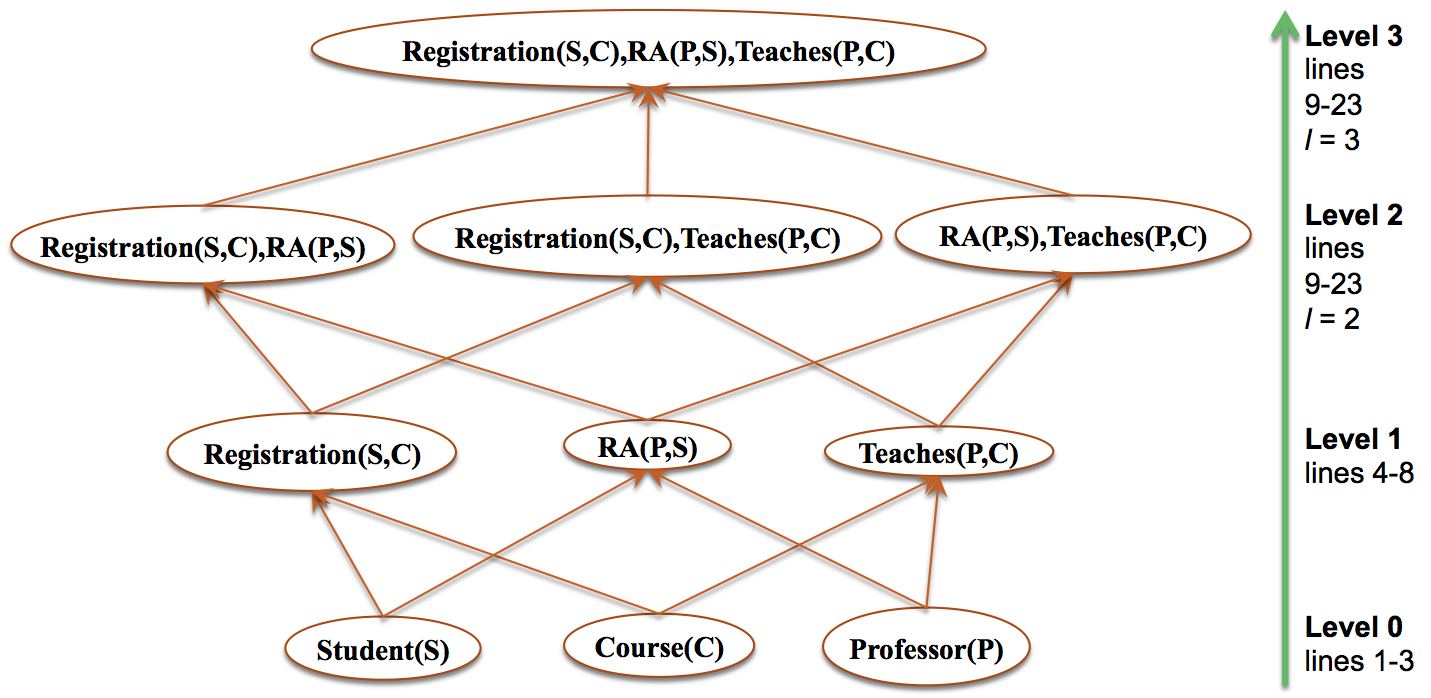
\includegraphics[width=0.9\textwidth]{uni-big-lattice.png}
}
\caption{A lattice of relationship sets for the university schema of Figure~\ref{fig:university-schema}. The M\"obius Join constructs contingency table tables for each relationship chain for each level $\ell$ of the lattice. I  reference the lines of the pseudo-code in Algorithm~\ref{alg:fmt}.
\label{fig:big-lattice}}
\end{center}
\end{figure}

With each relationship chain $\set{\Relation}$ (Rchain for short) is associated a $\ct$-table $\ct_{\set{\Relation}}$. The variables in the $\ct$-table  $\ct_{\set{\Relation}}$ comprise the relationship variables  in $\set{\Relation}$, and the unary/binary descriptive attributes associated with each of the relationships. To define these, I  introduce the following notation (cf. Table~\ref{table:translation}).

\begin{itemize}
\item  $\eatts(\A)$ denotes the attribute variables of a first-order variable $\A$ collectively (1 for unary).
\item $\eatts(\set{R})$ denotes the set of entity attribute variables for the first-order variables that are involved in the relationships in $\set{R}$. 
%\item $\eatts(\set{\R})$ is the union of the entity attributes for each relationship $\R \in \set{\R}$.
\item $\ratts(\set{R})$ denotes the set of relationship attribute variables for %the first-order variables involved in 
the relationships in $\set{R}$ (2 for binary).
%\item $\ratts(\set{R})$ is the union of the relationship attributes for each relationship $R \in \set{R}$.
\item $\atts(\set{R}) \equiv \eatts(\set{R}) \cup \ratts(\set{R})$ is the set of all attribute variables in the relationship chain $\set{R}$.
\end{itemize}

In this notation, the variables in the $\ct$-table  $\ct_{\set{\Relation}}$  are denoted as $\set{\Relation} \cup \atts({\set{R}})$. The goal of the M\"obius Join algorithm is to compute a contingency table for each chain $\set{\Relation}$. In the example of Figure~\ref{fig:big-lattice}, the algorithm computes 10 contingency tables. The $\ct$-table for the top element of the lattice is the \textbf{joint $\ct$-table} for the entire database. 




\section{Computing Contingency Tables For Positive Relationships} \label{sec:pos}

If a conjunctive query involves only positive relationships, then it can be computed using SQL's count aggregate function applied to a table join. This is relatively easy for a {\em fixed} set of par-RVs; the challenge is a general construction that works for different sets of par-RVs. 

{\em For a fixed set}, a  contingency table can be computed by an SQL count(*) query of the form 
\begin{quote}
CREATE VIEW CT-table  AS\\
SELECT COUNT(*) AS count, <VARIABLE-LIST>\\
FROM <TABLE-LIST>\\
GROUP BY <VARIABLE-LIST>\\
WHERE <Join-Conditions>
\end{quote}
To illustrate, I  also show one concrete SQL query for computing the positive relationship part of the $\ct$-table for the $\ra(\P,\S)$ chain.
\begin{quote}
CREATE VIEW $\ct_{T}$  AS 
\\SELECT COUNT(*) as  count,  \\ s.ranking, s.intelligence, p.popularity, p.teachingability, RA.capability, RA.salary  \\
FROM professor p, student s, RA  \\
WHERE  RA.p\_id = professor.p\_id and RA.s\_id = student.s\_id  \\
GROUP BY s.ranking,  s.intelligence, p.popularity,  p.teachingability, \\RA.capability,  RA.salary
\end{quote}
\subsection{Metaquery} \label {sub:meta}
{\em For the general construction}, I  describe how the contingency table problem can be solved using SQL with {\em metaqueries}. 
The FactorBase  uses SQL itself to construct the count-conjunction query. I  refer to this construction as an SQL \textbf{metaquery}. Thus an SQL metaquery maps schema information to the components of another SQL query. 

I  represent a count(*) query in four kinds of tables: the Select, From, Where and Group By tables. Each of these tables lists the entries in the corresponding count(*) query part.
The Select table lists the entries in the Select clause of the target query, the From table lists the entries in the From clause, and similar for Where and Group By tables. 
Given the four metaquery tables, the corresponding SQL count(*) query can be easily constructed and executed in an application to construct the contingency table.

Given a list of par-RVs as input, the metaquery tables are constructed as follows from the metadata in the database $\RVD$ as described in section \ref{chaSecRVD}.  
\begin{description}
\item[FROM LIST] Find the tables referenced by the \RRV's. A \RRV ~references the entity tables associated with its first-order variables (see VDB.Relationship\_FOvariables). Relational \RRV's also reference the associated relationship table (see VDB.Relationship). 
\item[WHERE LIST] Add join conditions on the matching primary keys of the referenced tables in the WHERE clause. The primary key columns are recorded in VDB. 
\item[SELECT LIST] For each attribute \RRV, find the corresponding column name in the original database (see VDB.AttributeColumns). Rename the column with the ID of the \RRV. Add a $\qcount$ column.
\item[GROUP BY LIST] The entries of the Group By table are the same as in the Select table without the $\qcount$ column.
\end{description}

% The metaquery accesses tables in the Relational Random Variable Database. %I  omit further details due to space constraints.

\begin{figure}[htb]
\begin{center}
\resizebox{0.9\textwidth}{!}{
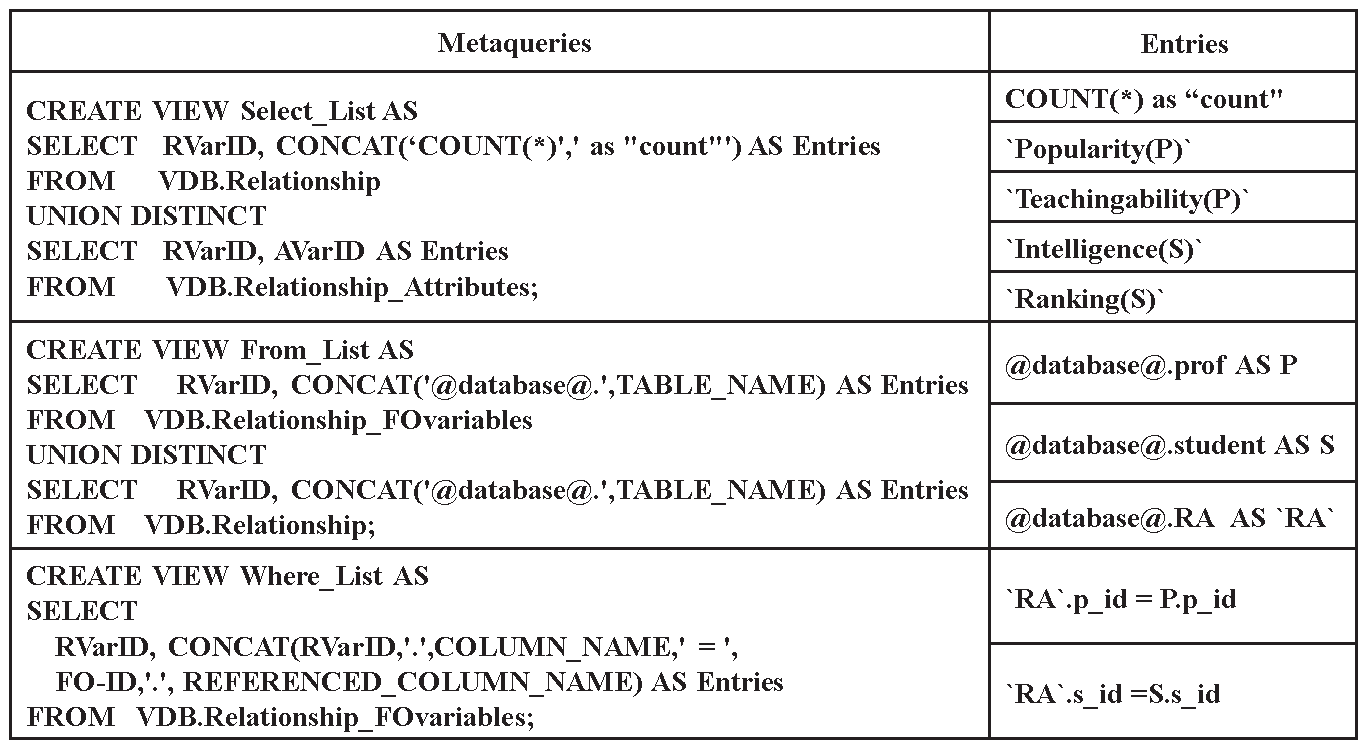
\includegraphics{meta-query.pdf}
}
\caption{Example of metaquery results based on university database and the par-RV metadata (Table \ref{table:vdb-schema}).
~\label{fig:meta-query}}
\end{center}
\end{figure}


Figure~\ref{fig:meta-query} shows an example of a metaquery for the university database. This metaquery defines a view that in turn defines a contingency table for the random variable list associated with the relationship table $\ra$. This list includes the entity attributes of professors and of students, as well as the relationship attributes of the $\ra$ relationship. 
The Bayesian network of Figure~\ref{fig:pbn} was learned from this contingency table. 
The  contingency table defined by the metaquery of Figure~\ref{fig:meta-query} contains only rows where the value of $\ra$ is true. 
%The M\"obius Virtual Join~\cite{Qian2014a} can be used to extend this contingency table to include counts for when $\ra$ is false, like the table shown in Figure~\ref{fig:pbn} (c).
Even more efficient than SQL count queries is the Tuple ID propagation method which could be used for computing query counts with positive relationships only \cite{Yin2004}. 

In the next section I  assume that contingency tables for positive relationships only have been computed already, and consider how such tables can be extended to full contingency tables with both positive and negative relationships (e.g, $\ra$ is true  and $\ra$ is  false). 



\section{Computing Contingency Tables For Negative Relationships} \label{sec:nag}

I  describe a Virtual Join algorithm that computes the required sufficient statistics without  materializing a cross product of entity sets. 
\begin{enumerate}
\item  I  introduce an  extension of relational algebra that I  term \textbf{contingency table algebra}. The purpose of this extension is to show that query counts using $k+1$ negative relationships can be computed from two query counts that each involve at most $k$ relationships. 
\item A dynamic programming algorithm applies the algebraic identify repeatedly to build up a complete contingency table from partial tables.
\end{enumerate}

\subsection{Contingency Table Algebra} \label{sec:cta}
I  introduce relational algebra style operations defined on contingency tables.

\subsubsection{Unary Operators} \label{sec:unary}
\begin{description}
\item[Selection] $\sigma_{\selectcond}  \ct$ selects a subset of the rows in the  $\ct$-table  that satisfy condition $\selectcond$. This is the standard relational algebra operation except that the selection condition $\selectcond$ may not involve the $\qcount$ column.
\item[Projection]  %$\project_{\set{V}}  
$\project_{\V_{1},\ldots,\V_{k}} \ct$ selects a subset of the  columns in the  $\ct$-table, excluding the count column. 
The counts in the projected subtable are the sum of counts of rows that satisfy the query in the subtable. 
The  $\ct$-table projection  $\project_{\V_{1},\ldots,\V_{k}} \ct$ can be defined by the following SQL code template:
\begin{quote}
SELECT SUM(count) AS count, $V_{1}, \ldots,\ V_{k}$ \\
FROM $\ct$ \\
GROUP BY $V_{1}, \ldots,\ V_{k}$
\end{quote}

\item[Conditioning]  $\condition_{\selectcond}  \ct$ returns a conditional contingency table. Ordering the columns as $(V_{1},\ldots,V_{k}, \ldots,\V_{k+j}$),  suppose that the selection condition is a conjunction of values of the form $$\selectcond = (V_{k+1} = v_{k+1},\ldots, V_{k+j} = v_{k+j}).$$  Conditioning can be defined in terms of selection and projection by the equation:
\begin{equation}
\condition_{\selectcond}  \ct = \project_{\V_{1},\ldots,\V_{k}} (\select_{\selectcond}  \ct) \nonumber
\end{equation}
\end{description}

\subsubsection{Binary Operators} \label{sec:bin}
I  use $\set{V}$, $\set{U}$ in SQL templates to denote a list of column names in arbitrary order. The notation $\ct_{1}.\set{V} = \ct_{2}.\set{V}$ indicates an equijoin condition: the contingency tables $\ct_{1}$ and $\ct_{2}$ have the same column set $\set{V}$ and matching columns from the different tables have the same values.
\begin{description}
\item[Cross Product] 
The \textbf{cross-product} of $\ct_{1}(\set{U}),\ct_{2}(\set{V})$ is the Cartesian product of the rows, where the product counts are the products of count. The cross-product can be defined by the following SQL template:
\begin{quote}
SELECT \\($\ct_{1}.\qcount *\ct_{2}.\qcount$) AS $\qcount$,  $\set{U}$, $\set{V}$\\
FROM  $\ct_{1},\ct_{2}$
\end{quote}


\item[Addition] 
 The \textbf{count addition} $\ct_{1}(\set{V}) + \ct_{2}(\set{V})$ adds the counts of matching rows, as in the following SQL template.
\begin{quote}
SELECT % $\ct_{1}$.COUNT+$\ct_{2}$.COUNT 
$\ct_{1}.\qcount$+$\ct_{2}.\qcount$ AS $\qcount$, $\set{V}$ \\%$\ct_{1}.V_{1} , \ldots, \ct_{1}.V_{k} $ \\
FROM  $\ct_{1},\ct_{2}$\\
%WHERE $\ct_{1}.V_{1} = \ct_{2}.V_{1}, \ldots, \ct_{1}.V_{k} = \ct_{2}.V_{k}$
WHERE $\ct_{1}.\set{V} = \ct_{2}.\set{V}$
\end{quote}

If a row appears in one $\ct$-table but not the other, I  include the row with the count of the table that contains the row. 

\item[Subtraction] %
The \textbf{count difference} $\ct_{1}(\set{V}) - \ct_{2}(\set{V})$ equals $\ct_{1}(\set{V}) + (- \ct_{2}(\set{V}))$ where $- \ct_{2}(\set{V})$ is the same as $\ct_{2}(\set{V})$ but with negative counts. 
Table subtraction is defined only if (i) without the $\qcount$ column, the rows in $\ct_{1}$ are a superset of those in $\ct_{2}$, and (ii) for each row that appears in both tables, the count in $\ct_{1}$ is at least as great as the count in $\ct_{2}$.
\end{description}

\subsubsection{Implementation}\label{sec:imp}
The selection operator can be implemented  using SQL as with standard relational algebra. Projection with $\ct$-tables requires use of the GROUP BY construct as shown in section~\ref{sec:unary} [Unary Operators]. %The most difficult operation to implement efficiently is 

For addition/subtraction, assuming that a sort-merge join is used \cite{Ullman1982}, a standard analysis shows that the cost of a sort-merge join is $\it{size}(table1) + \it{size}(table2) +$ the cost of sorting both tables. 

The cross product is easily implemented in SQL as shown in section~\ref{sec:bin} [Binary Operators]. The cross product size is quadratic in the size of the input tables.


\subsection{Lattice Computation of Contingency Tables} \label{sec:mobius}
This section describes a method for computing the contingency tables level-wise in the relationship chain lattice. I  start with a contingency table algebra equivalence that allows us to compute counts for rows with negative relationships from rows with positive relations. Following \cite{Moore1998}, I  use a ``don't care'' value $*$ to indicate that a query does not specify the value of a node. For instance, the query $\Relation_{1} = \true, \Relation_{2} = *$ is equivalent to the query $\Relation_{1} = \true$. 
\begin{figure*}[!h]
\begin{center}
\resizebox{1\textwidth}{!}{
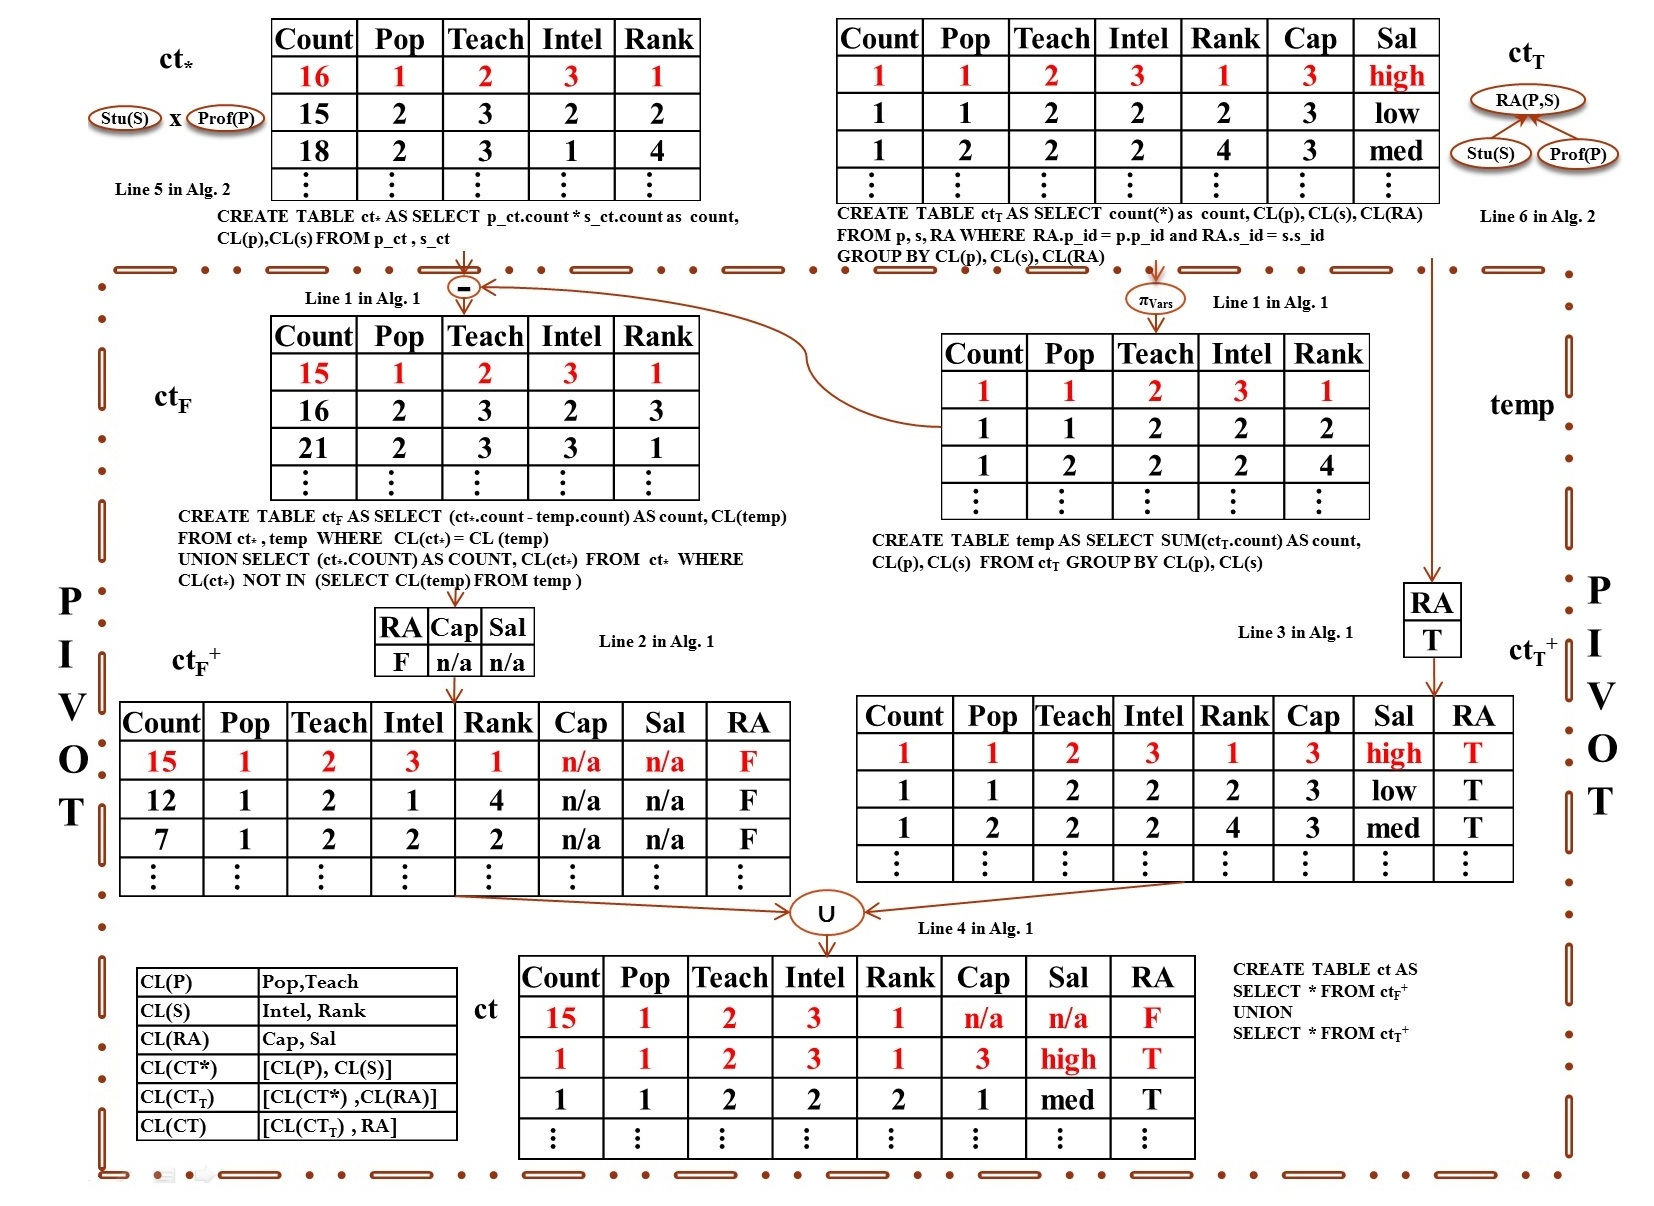
\includegraphics[width=1\textwidth]{sub.jpg}	
}
\caption{Top: Equation~\eqref{eq:update} is used to compute the conditional contingency table $\ct_{\false} = \ct(\eatts(R)|R = F)$. (Set $\Nodes = \emptyset$, $R = \ra(\P,\S)$, $\set{R} = \emptyset$). Bottom: 
The Pivot operation computes the contingency table $\ct_{\ra(\P,\S)}$ for the relationship $\ra(\P,\S) := \R_{pivot}$. The $\ct$-table operations are implemented using dynamic SQL queries as shown. Lists of column names are abbreviated as shown and also as follows.
$\ColumnList({\ct_{*}}) = \ColumnList({temp})=\ColumnList({\ct_{F}})$, 
$\ColumnList({\ct}) =  \ColumnList(\ct_{\false}^{+})  = \ColumnList(\ct_{\true}^{+}) $. I  reference the corresponding lines of Algorithms~\ref{Pivot_CT_Computation} and~\ref{alg:fmt}.
\label{fig:flow}}
\end{center}
\end{figure*}
%
%\SetAlFnt{\small}%cha:multiStatistic
\begin{algorithm*}[!h]
%\linesnumbered
\SetKwData{KwCalls}{Calls}
\SetKwData{KwCondition}{Precondition:}
\KwIn{Two conditional contingency tables   $\ct_{\true} :=\ct(\Nodes,\it{\ratts}(R_{\it{pivot}})|R_{\it{pivot}}=\true$$,\set{R}=\true)$ and  $\ct_{*} :=\ct(\Nodes|R_{\it{pivot}} = *$$,\set{R}=\true)$ .}
\KwCondition  %$\Nodes:= \eatts(\R_{1},\ldots,\R_{\ell}) \cup \ratts(\R_{1},\ldots,\R_{\ell}) \cup (\R_1,\ldots,\R_{\ell}) - R_{\it{pivot}} - \ratts(R_{\it{pivot}}) $ \;
 The set $\Nodes$ does not contain the relationship variable $R_{\it{pivot}}$ nor any of its descriptive attributes $\ratts(R_{\it{pivot}}$).\;
% {The set $\Nodes$ contains $\eatts(\R_{1},\ldots,\R_{\ell}) \cup \ratts(\R_{1},\ldots,\R_{\ell}) \cup (\R_1,\ldots,\R_{\ell})$ but not the relationship variable $R_{\it{pivot}}$ nor any of its descriptive attributes $\ratts(R_{\it{pivot}}$) \;}
\KwOut{The conditional contingency table $ \ct(\Nodes,\it{\ratts}(R_{\it{pivot}}),R_{\it{pivot}}|$$\set{R}=\true)$ .}
\begin{algorithmic}[1]
%\STATE $CT_{\false} := \ct(\Nodes|R_{\it{pivot}} = *$$,\set{R}=\true) - \pi_{\Nodes} \ct(\Nodes,\it{\ratts}(R_{\it{pivot}})|R_{\it{pivot}}=\true$$,\set{R}=\true)$.
\STATE $\ct_{\false} := \ct_{*} - \pi_{\Nodes}\ct_{\true}$.

\COMMENT{Implements the algebra Equation~\ref{eq:update} in proposition~\ref{PivotCT}.}
\STATE $\ct_{\false}^{+}$ := extend  $\ct_{\false}$ with columns $R_{\it{pivot}}$ everywhere false and $\it{\ratts}(R_{\it{pivot}})$ everywhere $n/a$.
%\STATE $CT_{\true}^{+}$ := extend  $\ct(\Nodes,\it{\ratts}(R_{\it{pivot}})|R_{\it{pivot}}=\true$$,\set{R}=\true)$ with columns $R_{\it{pivot}}$ everywhere true.
\STATE $\ct_{\true}^{+}$ := extend  $\ct_{\true}$ with columns $R_{\it{pivot}}$ everywhere true.
\STATE \Return $\ct_{\false}^{+} \cup \ct_{\true}^{+}$
\end{algorithmic}
\caption{The Pivot function returns a conditional contingency table for a set of attribute variables and all possible values of the relationship $R_{\it{pivot}}$, including $R_{\it{pivot}} = \false$. %It implements the algebra Equation~\eqref{eq:update}.
 The set of conditional relationships $\set{R} =(\R_{pivot},\ldots,\R_{\ell})$ %=\true$
 may be empty in  which case the Pivot computes an unconditional ct-table.\label{Pivot_CT_Computation} } 
\end{algorithm*}



\begin{proposition}%[Pivot_CT]
\label{PivotCT}
Let $R$ be a relationship variable and let $\set{R}$ be a set of relationship variables. Let $\Nodes$ be a set of variables that %(1) must contain all $\eatts$ of $\R$, and may contain any other variables, as long as (2) $\Nodes$ 
does not contain $\R$ nor any of the $\ratts$ of $\R$. Let  $\X_{1},\ldots, \X_{l}$ be the first-order variables that appear in $\R$ but not in $\Nodes$, where ${l}$ is possibly zero. Then I  have
\begin{flalign}
\label{eq:update}
&\ct(\Nodes \cup \eatts(R)|\set{R} = \true, R = F) = & \\ %\nonumber\\
& \ct(\Nodes|\set{R} = \true, R =*) \times \ct(\X_{1}) \times \cdots \times \ct(\X_{l}) \nonumber & \\
& -\ct(\Nodes  \cup \eatts(R)|\set{R} = \true, R = T). \nonumber&
\end{flalign}
If $l = 0$, the equation holds without  the %$ \ct(\X_{1}) \times \cdots \times \ct(\X_{k})$ 
cross-product term.
\end{proposition}

\begin{proof}
The equation 
\begin{align}
&\ct(\Nodes  \cup \eatts(R)|\set{R} = \true, R = *) = &\label{eq:update2}  \\ 
&\ct(\Nodes  \cup \eatts(R)|\set{R} = \true, R = T)  + & \nonumber \\ 
&\ct(\Nodes  \cup \eatts(R)|\set{R} = \true, R = F) & \nonumber
\end{align}
holds because the set $\Nodes \cup \eatts(R)$ contains all first-order variables in $R$.\footnote{I  assume here that  for each first-order variable, there is at least one $\eatt$, i.e., descriptive attribute.} % $\it{1Node}$. 
%
%Using table subtraction Equation~\eqref{eq:update} implies
 Equation~\eqref{eq:update2} implies
\begin{align} 
&\ct(\Nodes  \cup \eatts(R)|\set{R} = \true, R = \false) =& \label{eq:table-subtract} \\ 
&\ct(\Nodes  \cup \eatts(R)|\set{R} = \true, R = *) -&\nonumber  \\
 & \ct(\Nodes  \cup \eatts(R)|\set{R} = \true, R = \true).& \nonumber
\end{align}

To compute the $\ct$-table conditional on the relationship $\R$ being unspecified, I  use the equation
\begin{align}
&\ct(\Nodes  \cup \eatts(R)|\set{R} = \true, R = *) =  &\label{eq:table-multiply}\\
&\ct(\Nodes|\set{R} = \true, R =*) \times \ct(\X_{1}) \times \cdots \times \ct(\X_{l})& \nonumber
\end{align}
which holds because if the set $\Nodes$ does not contain a first-order variable of $\R$, then the counts of the associated $\eatts(\R)$ are independent of the counts for $\Nodes$. 
If $l = 0$, there is no new first-order variable, and Equation~\eqref{eq:table-multiply} holds without  the cross-product term.
%
Together Equations~\eqref{eq:table-subtract} and~\eqref{eq:table-multiply} establish the proposition.
\end{proof}

\begin{algorithm*}[!h]
\SetKwData{KwCalls}{Calls}
\SetKwData{Notation}{Notation}
\KwIn{A relational database $\D$; a set of  variables}
\KwOut{A contingency table that lists the count in the database $D$ for each possible assignment of values to each variable.}
\begin{algorithmic}[1]
\FORALL{first-order variables $\X$}
\STATE compute $\ct(\eatts(\X))$ using SQL queries.
\ENDFOR
\FORALL{relationship variable $\R$}
\STATE $\ct_{*} := \ct(\X) \times \ct(\Y)$ where $\X$,$\Y$ are the first-order variables in $\R$.
\STATE $\ct_{\true} := \ct(\eatts(\R)|\R = \true)$ using SQL joins.
\STATE Call  $\it{Pivot}(\ct_{\true},\ct_{*})$ to compute $\ct(\eatts(\R),\ratts(\R),\R)$.
\ENDFOR
\FOR{Rchain length $\ell=2$ to $m$}
\FORALL{Rchains $\set{\R} = R_{1},\ldots,\R_{\ell}$}
\STATE $Current\_\ct :=  \ct(\eatts(\R_{1},\ldots,\R_{\ell}),\ratts(\R_{1},\ldots,\R_{\ell})|\R_{1}=\true,\ldots,\R_{\ell}=\true)$ using SQL joins.
\FOR{$i=1$ to $\ell$} \label {refline:innerloop}
\IF{ $i$ equals  1}
\STATE $\ct_{*} := \ct(\eatts(\R_{2},\ldots,\R_{\ell}),\ratts(\R_{2},\ldots,\R_{\ell})|
\R_{1}=*,\R_{2} = \true,\ldots,\R_{\ell}=\true) \times \ct(\X)$ where $\X$ is the first-order variable in $\R_{1}$, if any, that does not appear in $\R_{2},\ldots,\R_{\ell}$
\COMMENT{$\ct_{*}$ can be computed from a $\ct$-table for a Rchain of length $\ell-1$.}
\ELSE
\STATE $\eatts_{\bar{i}} := \eatts(\R_{1},\ldots,\R_{i-1},\R_{i+1},\ldots,\R_{\ell})$.
\STATE $\ratts_{\bar{i}} := \ratts(\R_{1},\ldots,\R_{i-1},\R_{i+1},\ldots,\R_{\ell})$.
\STATE $\ct_{*} := \ct(\eatts_{\bar{i}}, \ratts_{\bar{i}},\R_{1},\ldots,\R_{i-1})|
\R_{i}=*,\R_{i+1} = \true,\ldots,\R_{\ell}=\true) \times \ct(\Y)$ where $\Y$ is the first-order variable in $\R_{i}$, if any, that does not appear in $\set{\R}$. 
\ENDIF \\
\STATE $Current\_\ct :=  \it{Pivot}(Current\_\ct,\ct_{*})$.
\ENDFOR 
\COMMENT{Loop Invariant: After  iteration $i$, the table $Current\_\ct$ equals 
$\ct(\eatts(\R_{1},\ldots,\R_{\ell}), \ratts(\R_{1},\ldots,\R_{\ell}),\R_{1},\ldots,\R_{i}|\R_{i+1} = \true,\ldots,\R_{\ell}=\true)$}
\ENDFOR
\COMMENT{Loop Invariant: The $\ct$-tables for all Rchains of length $\ell$ have been computed.}
\ENDFOR 
\STATE \Return the $\ct$-table for the Rchain involves all the relationship variables.
\end{algorithmic}
\caption{M\"obius Join algorithm for Computing the Contingency Table for Input Database. \label{alg:fmt}}
\end{algorithm*}
%The proof is available at \cite{techreport}. 

Figure~\ref{fig:flow} illustrates Equation~\eqref{eq:update}. 
The construction of the $\ct_{\false}$ table in Algorithm~\ref{Pivot_CT_Computation} provides pseudo-code for applying Equation~\eqref{eq:update} to compute a complete $\ct$-table, given a partial table where a specified relationship variable $\Relation$  is true, and another partial table that does not contain the relationship variable. 
I  refer to $\Relation$ as the \textbf{pivot} variable. For extra generality, Algorithm~\ref{Pivot_CT_Computation} applies Equation~\eqref{eq:update} with a condition that lists a set of relationship variables fixed to be true.  Figure~\ref{fig:flow} illustrates the  Pivot computation for the case of only one relationship. 
Algorithm~\ref{alg:fmt} shows how the Pivot operation can be applied repeatedly to find all contingency tables in the relationship lattice. 


{\em Initialization.} Compute $\ct$-tables for entity tables.
% (lines 1--3). 
Compute $\ct$-tables for each single relationship variable $\Relation$ , conditional on $\Relation = \true$. % (line 6).  
If $\Relation = \ast$, then no link is specified between the first-order variables involved in the relation $\Relation$. Therefore the individual counts for each first-order variable are independent of each other and the joint counts can be obtained by the cross product operation. % (line 5). 
Apply the Pivot function to construct the  complete $\ct$-table for relationship variable $\Relation$. % (line 7). 

{\em Lattice Computation.} The goal is to compute $\ct$-tables for all relationship chains of length $>1$. For each relationship chain, order the relationship variables in the chain arbitrarily. Make each relationship variable in order the Pivot variable $\Relation_{i}$. For the current Pivot variable $\Relation_{i}$, find the conditional $\ct$-table where $\Relation_{i}$ is unspecified, and the subsequent relations $\Relation_{j}$ with $j>i$ are true. This $\ct$-table can be computed from a $ct$-table for a shorter chain that has been constructed already. The conditional $ct$-table   has been constructed already, where $\Relation_{i}$ is true, and the subsequent relations are true (see loop invariant). Apply the Pivot function to construct the  complete $\ct$-table, for any Pivot variable $\Relation_{i}$,  conditional on the subsequent relations being true. 
%Figure~\ref{fig:rchain-loop} illustrates the loop over the relationship chain members for the relationship chain $\reg(\S,\C),\ra(\P,\S).$

\begin{figure}[htbp]
\begin{center}
\resizebox{1\textwidth}{!}{
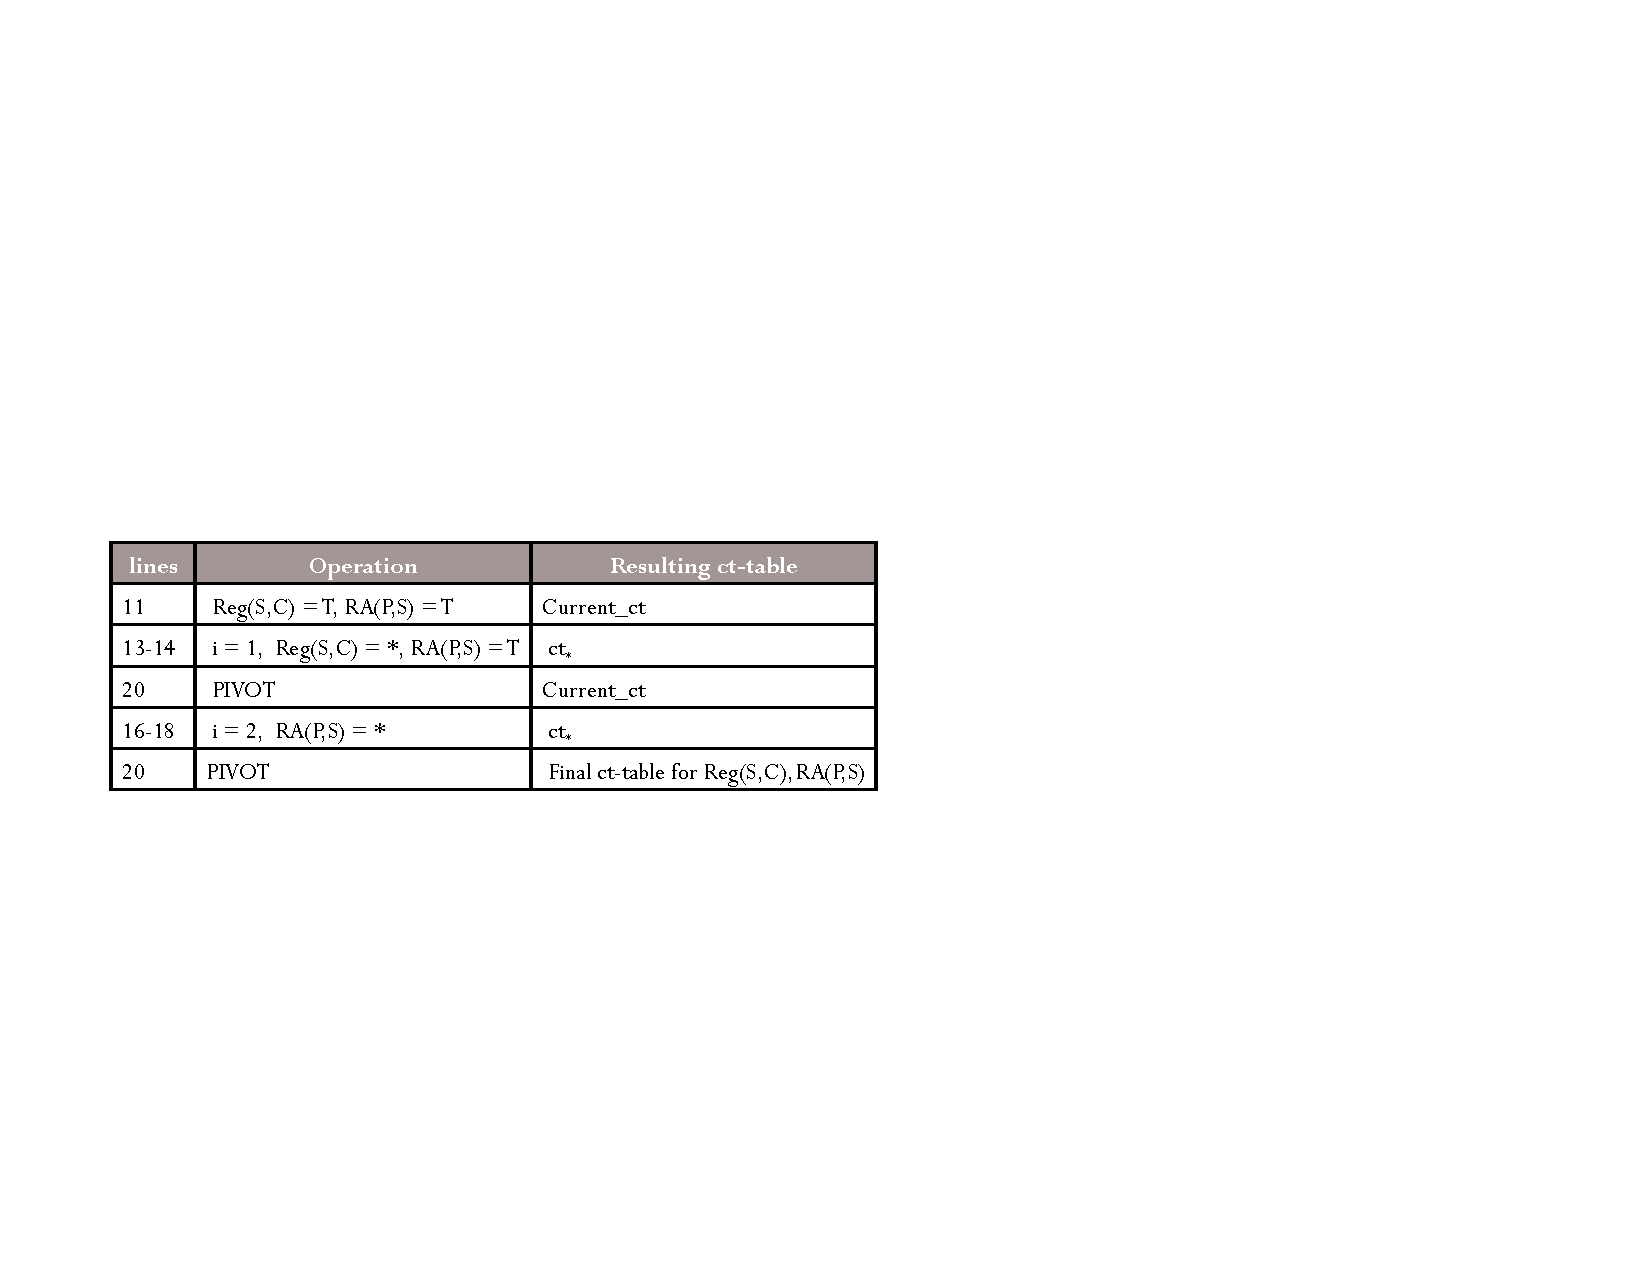
\includegraphics{rchain-loop.pdf}}
\caption{Illustrates the relationship chain loop of Algorithm~\ref{alg:fmt} (lines 11-21) for the chain $\set{\R}= \it{Reg}(\S,\C),\ra(\P,\S)$. This loop is executed for each relationship chain at each level.
\label{fig:rchain-loop}}
\end{center}
\end{figure}



\subsection{Complexity Analysis} \label{sec:complexity1} 

The key point about the M\"obius Join (\MJ) algorithm is that it avoids materializing the cross product of entity tuples. {\em The algorithm accesses  only \textbf{existing} tuples, never constructs nonexisting tuples.} The number of $\ct$-table operation is therefore independent of the number of data records in the original database. 
The Virtual Join algorithm scales well with the number of rows, but not with the number of columns and relationships in the database. This limitation stems from the fact that the contingency table size grows exponentially with the number of random variables in the table. 

I  bound the total number of $\ct$-algebra operations performed by the M\"obius Join algorithm in terms of the size of its output: the number of sufficient statistics that involve negative relationships. 

\begin{proposition}
The number of $\ct$-table operations performed by the M\"obius Join algorithm is bounded as $$\it{\# \ct\_\it{ops}} = O(r \cdot \log_{2} r)$$ where $\row$ is the number of sufficient statistics that involve negative relationships.
\end{proposition}



To  analyze the computational cost, I  examine the total number of $\ct$-algebra operations performed by the  M\"obius Join algorithm. 
%
I  provide  upper bounds in terms of two parameters: the number of relationship nodes  $m$, and  the number of rows $\row$  in the $\ct$-table that involve negative relationships.
For these parameters I  establish that
$$\it{\# \ct\_\it{ops}} = O(r \cdot \log_{2} r) = O(m \cdot 2^{m}) .$$
This shows the efficiency of the algorithm for the following reasons.
(i) Since the time cost of any algorithm must be at least as great as the time for writing the output, which is as least as great as $\row$, 
 the  M\"obius Join algorithm adds at most a logarithmic factor to this lower bound. 
(ii)  The second upper bound means that the number of $\ct$-algebra operations is fixed-parameter tractable with respect to $m$.\footnote{For arbitrary $m$, the problem of computing a $\ct$ table in a relational structure is \#P-complete \cite[Prop.12.4]{Domingos2007}.} In practice the number $m$ is on the order of the number of tables in the database, 
which is very small compared to the number of tuples in the tables.

\emph{Derivation of Upper Bounds.}
For a given relationship chain of length $\ell$,  the  M\"obius Join algorithm goes through the chain linearly (Algorithm~\ref{alg:fmt} 
inner for loop line~\ref{refline:innerloop}%12
). 
% check line number
At each iteration, it computes a $\ct_{*}$ table with a single cross product, then performs a single Pivot operation.  Each Pivot operation requires three  $\ct$-algebra operations. Thus overall, the number of  $\ct$-algebra operations for a relationship chain of length $\ell$ is $6 \cdot \ell = O(\ell)$. For a fixed length $\ell$, there are at most $\binom{m}{\ell}$ relationship chains. Using the known identity\footnote{math.wikia.com/wiki/Binomial\_coefficient, Equation 6a}
\begin{align} 
\sum_{\ell=1}^{m} {m\choose \ell} \cdot \ell = m \cdot  2^{m-1} \label{eq:upperbound}
\end{align}
I  obtain the $O(m \cdot  2^{m-1}) = O(m \cdot  2^{m})$ upper bound.%{http://goo.gl/x65yl3}. 
%\textbf{URL}
%With the Binomial theorem the identity ~\eqref{eq:upperbound} is easy to prove, I  omit further details due to space constraints.

Here I  give a quick proof of the identity ~\eqref{eq:upperbound}. 
\begin{proof}
With the Binomial theorem, for any non-negative integers $l,m$, the binomial formula of two variables $a,b$ is 
$$ f(a,b)=\sum_{\ell=0}^{m}\binom{m}{\ell} \cdot a^{m-\ell} \cdot b^\ell = (a+b)^m. $$
Suppose I  substitute $a$ with one, for any $b$, I  have 
$$
f(1,b)= \sum_{\ell=0}^m\binom{m}{\ell} \cdot b^\ell=(1+b)^m.
$$
And then I  could compute the partial derivative with respect to $b$
$$
f'_{b}(1,b)= \sum_{\ell=1}^m\binom{m}{\ell}\cdot \ell \cdot b^{\ell-1}=m \cdot (1+b)^{m-1}.$$
By substituting $b$ with one, we end the proof 
$$f'_{b}(1,1)=  \sum_{\ell=1}^m\binom{m}{\ell}\cdot \ell \cdot 1^{\ell-1}= \sum_{\ell=1}^m\binom{m}{\ell}\cdot \ell = m\cdot(2)^{m-1}.$$

%That means the following identity
%$$\sum_{\ell=1}^{m} {m\choose \ell}\cdot \ell = m * 2^{m-1}  $$ holds.
\end{proof}

For the upper bound in terms of $\ct$-table rows $\row$, I  note that the output $\ct$-table can be decomposed into $2^{m}$ subtables, one for each assignment of values to the $m$ relationship nodes. 
Each of these subtables contains the same number of rows $d$ , one for each possible assignment of values to the attribute nodes. 
Thus the total number of rows is given by $r = d \cdot 2^m.$ 
Therefore I  have 
$m \cdot 2^{m} = \log_{2} (r/d) \cdot r/d \leq \log_{2}(r) \cdot r.$
Thus the total number of $\ct$-algebra operations is $O(r \cdot \log_{2}(r))$.
%$\it{\# \ct\_\it{ops}} = O(r \cdot \log r) .$

From this analysis I  see that both upper bounds are overestimates. (1) Because relationship chains must be linked by foreign key constraints, the number of valid relationship chains of length $\ell$ is usually much smaller than the number of all possible subsets ${m\choose \ell}$. (2) The constant factor $d$ grows exponentially with the number of attribute nodes, so $\log_{2}(r) \cdot r$ is a loose upper bound on $\log_{2} (r/d) \cdot r/d$. 
I  conclude that the number of $\ct$-algebra operations is not the critical factor for scalability, but rather the cost of carrying out a single $\ct$-algebra operation. 

In the benchmark datasets, the number of sufficient statistics was feasible, as I  report below. 
In Section~\ref{sec:conclusion} below I  discuss options in case the number of sufficient statistics  grows too large.


\begin{table}[htbp]
  \centering
  \caption{Notations for time complexity analysis}
    \begin{tabular}{|l|c|}\hline
    number of relationship tables & $m$ \\ \hline
    number of entity tables & $k$ \\ \hline
    size of entity table rows (domain) & $n$ \\ \hline
    size of relationship table rows & $j$ \\ \hline
    number of attribute columns (predicates) & $c$ \\ \hline
    number of values per attributes & $v$ \\ \hline
  %  length of the largest relationship chain & $\ell$  \\ \hline
    number of sufficient statistics for true relationships only & $\statistics$ = $v^{c}*m$    \\ \hline
    number of sufficient statistics for positive and negative relationships& $ss$ = $v^{c}*m*2^{m} $\\ \hline
    time complexity of Virtual Join algorithm  with respect to $\statistics$  & $O(\statistics * (2^{m}-1))$\\ \hline
    number of rows for all cross table join & $cp$ = $n^{k}*j^{m}$ \\ \hline
   % number of rows for largest cross table join & $n^{k}*j^{\ell}$ \\ \hline
    the compression ratio of $cp$ over $ss$  & $cr = \frac{cp}{ ss}$ \\ \hline
    \end{tabular}%
  \label{tab:input-complexity}%
\end{table}%


\paragraph{Time Complexity Analysis in terms of input raw database.}
The Virtual Join algorithm scales well with the number of rows, but not with the number of columns and relationships in the database. This limitation stems from the fact that the contingency table size grows exponentially with the number of random variables in the table. 
%My following complexity analysis confirms the fact. 

To  analysis the time complexity in terms of the input raw database with multiple tables, I  introduce the notations for some important parameters (cf. Table~\ref{tab:input-complexity}). Let $\statistics$ be the number of sufficient statistics where all relationship variables are true. For instance, if there are $c$ attributes, the number of values per attributes is $v$, then $\statistics = v^{c}*m$. 
The number of sufficient statistics for the whole input database with positive and negative relationships can be represented as $$ ss = v^{c}*m*2^{m}.$$
Then I  have $$ \row  =  v^{c}*m * (2^{m}-1)  = \statistics * (2^{m}-1), $$ since there are $2^{m}-1$ combinations of relationship values with at least one negative relationship.  So the time complexity of Virtual Join algorithm with respect to $\statistics$ is $$O(\statistics * (2^{m}-1)).$$
The experiments in section \ref{sec:jct} will demonstrate the compression ratio $cr$  is an important parameter as well.  Give the notations in Table~\ref{tab:input-complexity}, I  establish that $$ cr = \frac {cp} {ss} = \frac{n^{k}*j^{m}}{ v^{c}*2^{m}}. $$ These numbers align into two independent computational spaces. 
Generally the higher the compression ratio, the higher the time savings. However, if the compression ratio is unusually low, so materializing the cross-product was faster. For further depth analysis of how $cr$ will affect the performance of the Virtual Join algorithm, I leave it to future work.





\section{Evaluation of Contingency Table Computation: Scalability} \label{sec:data}


\subsection{Datasets}

I  used seven benchmark real-world databases. For detailed descriptions and  the sources of the databases, please see reference~\cite{Schulte2012}. Table~\ref{table:datasetsize} summarizes basic information about the benchmark datasets.  A  self-relationship %\cite{Heckerman+al:SRL07} 
relates two entities of the same type (e.g. $\it{Borders}$ relates two countries in Mondial). Random variables for each database were defined as described in Section~\ref{sec:variables} (see also \cite{Schulte2012}). IMDb is the largest dataset in terms of number of total tuples (more than 1.3M tuples) and schema complexity. %attributes.
It combines the MovieLens database\footnote{www.grouplens.org, 1M version} with data from the Internet Movie Database (IMDb)\footnote{www.imdb.com, July 2013} following \cite{Peralta2007}.


\begin{figure}[!h]
\begin{center}
\resizebox{1\textwidth}{!}{
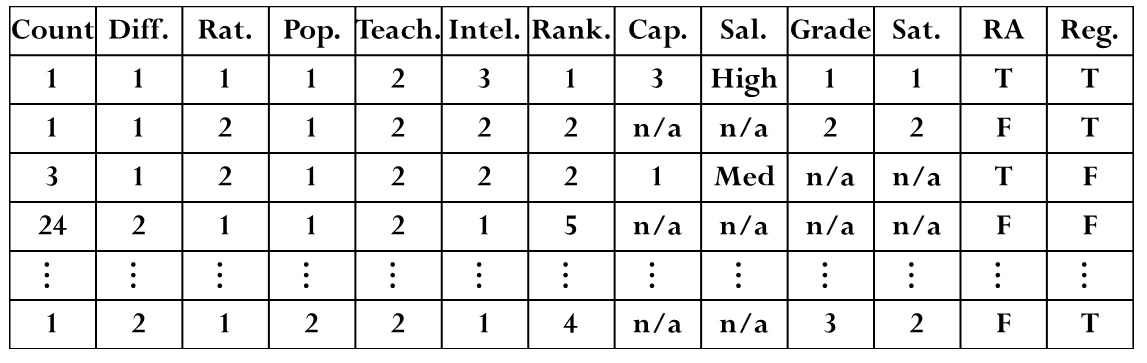
\includegraphics[width=1\textwidth]{uni-ct-table.JPG}
}
\caption{Excerpt from the joint contingency table for the university database of Figure~\ref{fig:university-tables}. 
\label{fig:ct}}
\end{center}
\end{figure}
\begin{table}[!h] \centering\caption{Datasets characteristics.\\ \#Tuples = total number of tuples over all tables in the dataset. 
  \label{table:datasetsize}}
\resizebox{1\textwidth}{!}{
\begin{tabular}[c]
{|l|c|c|r|c|}\hline
 \textbf{Dataset} & \textbf{\begin{tabular}[l] {ll} \#Relationship \\Tables/ Total \end {tabular}} & \textbf{\begin{tabular}[l] {ll} \#Self \\Relationships\end {tabular}}  & \textbf{\#Tuples} & \textbf{\#Attributes}  \\\hline
    Movielens &1 / 3 & 0  & 1,010,051 & 7\\\hline
    Mutagenesis & 2 / 4 & 0 & 14,540 & 11\\\hline
    Financial &3 / 7 & 0  &  225,932& 15\\\hline
   Hepatitis &3 / 7 & 0 &12,927  & 19\\\hline
   IMDb &3 / 7 & 0 &1,354,134  & 17\\\hline
    Mondial &2 / 4 & \textbf{1} &  870& 18\\\hline
    UW-CSE &2 / 4 & \textbf{2}  & 712 & 14\\\hline   
\end{tabular}
}
\end{table}



\subsection{Joint Contingency Tables With Negative Relationships}\label{sec:jct} %: Cross Product vs. M\"obius Join}
In this subsection I  compare two different approaches for constructing the {\em joint contingency tables} for all variables together, for each database: \textbf{the M\"obius Join algorithm (MJ) } vs. \textbf{materializing the cross product (CP) }of the entity tables for each first-order variable (primary keys).
Cross-checking the MJ contingency tables with the cross-product contingency tables confirmed the correctness of the implementation. 
Figure~\ref{fig:ct} shows the  joint contingency table for the university database. The value of a relationship attribute is undefined for entities that are not related.

Table~\ref{table:cttimes} compares the time and space costs of the MJ vs. the CP approach. The cross product was materialized using an SQL query. 
%The size of this cross product is identical to the sum of counts in the $\ct$-table, reported in Table~\ref{table:cttimes}. 
The ratio of the cross product size to the number of statistics in the $\ct$-table measures how much compression the $\ct$-table provides compared to enumerating the cross product. It shows that cross product materialization  requires an infeasible amount of space resources. The $\ct$-table provides a substantial compression of the statistical information in the database, by a factor of over 4,500 for the largest database IMDb.  

\begin{table}[!h] \centering
\caption{Constructing the contingency table for each dataset. \\
M = million. N.T. = non-termination. Compress Ratio = CP-\#tuples/\#Statistics. \\
Computation times are given in seconds. 
  \label{table:cttimes}}
\resizebox{1\textwidth}{!}{
\begin{tabular}{|l|r|r|r|r|r|}\hline 
 \textbf{Dataset} & \textbf{MJ-time}(s) & $\textbf{CP-time}(s)$& \textbf{CP-\#tuples}  & \textbf{\#Statistics} & \textbf{\begin{tabular}{l}Compress \\Ratio
 \end{tabular}} \\\hline
Movielens &2.70&703.99 &23M &252 &93,053.32\\\hline
Mutagenesis &1.67&1096.00 & 1M &1,631 &555.00  \\\hline
Financial &  1421.87&N.T. &149,046,585M &3,013,011 &49,467,653.90   \\\hline
Hepatitis &3536.76&N.T. &17,846M& 12,374,892 &1,442.19 \\\hline
IMDb &7467.85&N.T. &5,030,412,758M&15,538,430 & 323,740,092.05 \\\hline
Mondial &1112.84&132.13&5M&1,746,870&2.67  \\\hline
UW-CSE &3.84&350.30& 10M&2,828 & 3,607.32\\\hline
\end{tabular}
}

\end{table}



\paragraph{ Computation Time.} The numbers shown are the complete computation time for all statistics. For faster processing, both methods used a B+ tree index built on each column in the original dataset. The \MJ method also utilized B+ indexes on the $\ct$-tables. I  include the cost of building these indexes in the reported time. 
The M\"obius Join algorithm returned a contingency table with negative relationships in feasible time. On the biggest dataset IMDb with 1.3 million tuples, it took just over 2 hours. 


The cross product construction did not always terminate, crashing after around 4, 5, and 10 hours on Financial, IMDb and Hepatitis respectively. When it did terminate, it took orders of magnitude longer than the \MJ ~method except for the Mondial dataset. Generally the higher the compression ratio, the higher the time savings. On Mondial the compression ratio is unusually low, so materializing the cross-product was faster. 




\subsection{Contingency Tables with Negative Relationships vs. Positive Relationships Only} 
In this section I  compare \textbf{the time and space costs} of computing both positive and negative relationships, vs. positive relationships only.
I  use the following terminology. \textbf{Link Analysis On} refers to using a contingency table with sufficient statistics for both positive and negative relationships. 
An example is table $\ct$ in Figure~\ref{fig:flow}. 
\textbf{Link Analysis Off} refers to using a contingency table with sufficient statistics for positive relationships only. An example is table $\ct_{\true}^{+}$ %$\ct_{T^{+}}$
 in Figure~\ref{fig:flow}.  Table~\ref{table:link-onoff} shows the  number of sufficient statistics required for link analysis on vs. off. The difference between the link analysis on statistics  and the link analysis off statistics is the number of Extra Statistics.
 
 \begin{table}[!h]
  \centering
  \caption{Number of Sufficient Statistics for Link Analysis On and Off. \\Extra Time refers to the total \MJ time (Table~\ref{table:cttimes} Col.2) minus the time for computing the positive statistics only.}
  \label{table:link-onoff}%
\resizebox{1\textwidth}{!}{
\begin{tabular}{|l|r|r|r|r|}\hline
Dataset & \multicolumn{1}{r|}{Link On} & \multicolumn{1}{c|}{Link Off} & \multicolumn{1}{c|}{\#extra  statistics} & \multicolumn{1}{c|}{extra time (s)}    \\ \hline
MovieLens & 252   & 210   & 42    & 0.27    \\ \hline
Mutagenesis & 1,631 & 565   & 1,066 & 0.99    \\ \hline
Financial & 3,013,011 & 8,733 & 3,004,278 & 1416.21    \\ \hline
Hepatitis & 12,374,892 & 2,487 & 12,372,405 & 3535.51    \\ \hline
IMDb & 15,538,430 & 1,098,132 & 14,440,298 & 4538.62    \\ \hline
Mondial & 1,746,870 & 0     & 1,746,870 & 1112.31    \\ \hline
UW-CSE & 2,828 & 2     & 2,826 & 3.41    \\ \hline
\end{tabular}%
}  
\end{table}%
 
The Extra Time column shows how much time the \MJ algorithm requires to compute the Extra Statistics {\em after} the contingency tables for positive relationships are constructed using SQL joins.


 As Figure~\ref{fig:runtime-vj} illustrates, the Extra Time stands in a nearly linear relationship to the number of Extra Statistics, which confirms the analysis of Section~\ref{sec:complexity1}. Figure~\ref{fig:breakdown-vj} shows that most of the \MJ run time is spent on the Pivot component (Algorithm~\ref{Pivot_CT_Computation}) rather than the main loop (Algorithm~\ref{alg:fmt}). In terms of $\ct$-table operations, most time is spent on subtraction/union rather than cross product.
\begin{figure}[!h]
\begin{center}
\resizebox{1\textwidth}{!}{
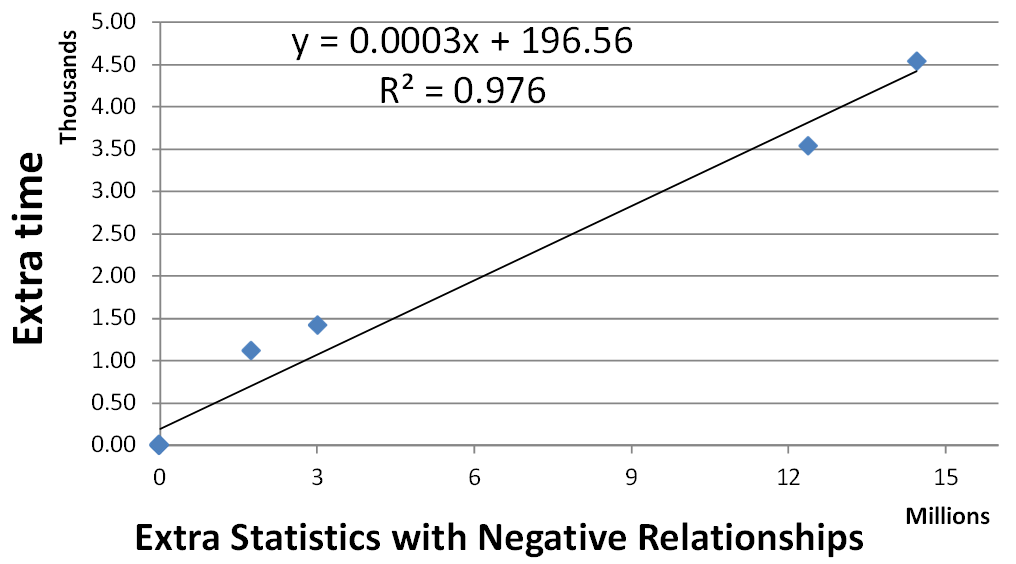
\includegraphics{extra_time.png}
}

\caption{M\"obius Join Extra Time (s)
\label{fig:runtime-vj}}
\end{center}
\end{figure}



\begin{figure}[!h]
\begin{center}
\resizebox{1\textwidth}{!}{
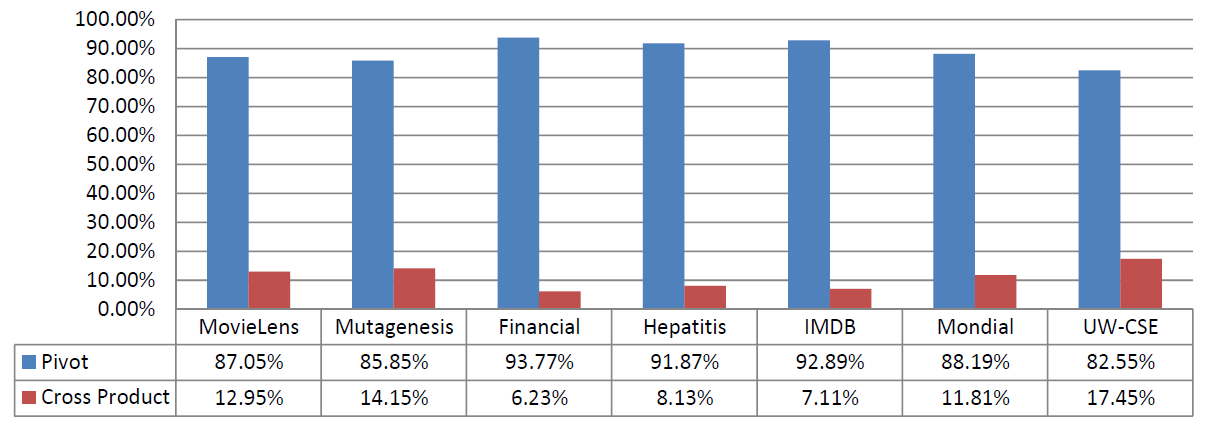
\includegraphics[width=1\textwidth]{sep_time.png}
}
\caption{Breakdown of \MJ Total Running Time
\label{fig:breakdown-vj}}
\end{center}
\end{figure}



\section{Evaluation of Statistical Applications: Usefulness}
I evaluate the usefulness on two different types of cross-table statistical analysis: feature selection and association rule  mining.%, and learning a Bayesian network.

\subsection{Feature Selection} 
For each database, I  selected a target for classification, then used Weka's CFS\footnote{The Correlation Feature Selection (CFS) measure evaluates subsets of features on the basis of the following hypothesis: ``Good feature subsets contain features highly correlated with the classification, yet uncorrelated to each other''\cite{Hall1999}.} feature subset selection method (Version 3.6.7) to select features for classification \cite{Hall2009}, given a contingency table. The idea is that if the existence of relationships is relevant to classification, then there should be a difference between the set selected with link analysis on and that selected with link analysis off. 
%Weka accepts instance weights as inputs, so its functions can be applied directly with contingency tables. 
I  measure how different two feature sets are by 1-Jaccard's coefficient:
$$\it{Distinctness}(A,B) = 1- \frac{A \cap B}{A \cup B}.$$

\begin{table}[!h] \centering
\caption{Selected Features for Target variables for  Link Analysis Off vs. Link Analysis On. Rvars denotes the number of relationship features selected. 
\label{table:feature-select}}
\resizebox{1\textwidth}{!}{
\begin{tabular}{|l|R{3cm}|R{2cm}|R{3cm}|r|} \hline
{\multirow{2}[4]{*}{Dataset}} &{\multirow{2}[4]{*}{Target variable}} & \multicolumn{2}{c|}{\# Selected Attributes} & {\multirow{2}[4]{*}{Distinctness}}\\ \cline{3-4} 
 & & Link Analysis Off & Link Analysis On / Rvars & \\\hline
MovieLens & Horror(M) & 2 & 2 / 0 &  0.0 \\\hline
Mutagenesis & inda(M) & 3 & 3 / 0 & 0.0 \\\hline
Financial & balance(T) & 3 & 2 / 1 & 1.0 \\\hline
Hepatitis & sex(D) & 1 & 2 / 1 & 0.5 \\\hline
IMDb & avg\_revenue(D) & 5 & 2 / 1 & 1.0 \\\hline
Mondial & percentage(C) & Empty CT  & 4 / 0 & 1.0 \\\hline
UW-CSE & courseLevel(C) & 1 & 4 / 2 & 1.0 \\\hline
\end{tabular}
}

\end{table}

Distinctness measures how different the selected feature subset is with link analysis on and off, on a scale from 0 to 1. Here 1 = maximum dissimilarity. Table~\ref{table:feature-select} compares the feature sets selected. In almost all datasets, sufficient statistics about negative relationships generate new relevant features for classification. %as indicated by standard relevance metrics. 
In 4/7 datasets, the feature sets are disjoint (coefficient = 1). For the Mutagenesis and MovieLens data sets, no new features are selected. 


\subsection{Association Rules} A widely studied task is finding interesting association rules in a database. I  considered association rules of the form $\it{body} \rightarrow \it{head}$, where $\it{body}$ and $\it{head}$ are conjunctive queries. An example of a cross-table association rule for Financial is 
%
$$\it{statement\_freq.(Acc)} = \it{monthly} \rightarrow \it{HasLoan}(\it{Acc},\it{Loan}) = \true.$$
I  searched for interesting rules using both the link analysis off and the link analysis on contingency tables for each database. The idea is that if a relationship variable is relevant for other features, it should appear in an association rule. With link analysis off, all relationship variables always have the value $\true$, so they do not appear in any association rule. I  used Weka's Apriori\footnote{Apriori heuristic: if any length k pattern is not frequent in the database, its length (k + 1) super-pattern can never be frequent \cite{Agrawal1994}} implementation to search for association rules in both modes. The interestingness metric was Lift\footnote{Let {\X} be an item-set,  and ${\X} \rightarrow {\Y}$ be an association rule. The \textbf{Lift} value of this rule is defined as  the ratio of the observed support to that expected if {\X}  and {\Y}  were independent. }. Parameters were set to their default values. Table~\ref{table:association} shows the number of rules that utilize relationship variables with link analysis on, out of the top 20 rules. In all cases, a majority of rules utilize relationship variables,  in Mutagenesis and IMDb all of them do. %\textbf{false relationships? usually yes} 
%
\begin{table}[h] \centering
\caption{Number of top 20 Association Rules that utilize relationship variables.}
  \label{table:association}%
\resizebox{1\textwidth}{!}{
\begin{tabular}{|c|c|c|c|c|c|c|c|}
\hline
\multicolumn{1}{|c|}{Dataset} & MovieLens & Mutagenesis & Financial & Hepatitis & IMDb  & Mondial & UW-CSE \\
\hline
\# rules  & 14/20  & 20/20 & 12/20 & 15/20 & 20/20 & 16/20 & 12/20 \\ %invovle rvariable
\hline %invovle rvariable
\end{tabular}%
}

\end{table}%



\section{Conclusion}\label{sec:conclusion}
Utilizing the information in a relational database for statistical modelling and pattern mining requires fast access to multi-relational sufficient statistics, that combine information across database tables. I  presented an efficient dynamic program that computes sufficient statistics for any combination of positive {\em and} negative relationships, starting with a set of statistics for positive relationships only. My dynamic program performs a Virtual Join operation, that counts the number of statistics in a table join without actually constructing the join. I  showed that the run time of the algorithm is $O(r \log r)$, where $r$ is the number of sufficient statistics to be computed. The computed statistics are stored in contingency tables. I  introduced contingency table algebra, an extension of relational algebra, to elegantly describe and efficiently implement the dynamic program. Empirical evaluation on seven benchmark databases demonstrated the scalability of the algorithm; I  compute sufficient statistics with positive and negative relationships in databases with over 1 million data records.  The experiments illustrated how access to sufficient statistics for both positive and negative relationships enhances feature selection and rule mining.%, and Bayesian network learning.  

While I  have focused on statistical analysis, one potential application is to complement the traditional ETL (extraction/transformation/loading) tasks~\cite{Han2011}. The ETL + single table machine learning training based model can take advantage of the extra sufficient statistics by incorporating both positive and negative relationships. This  could reduce the information loss caused by propositionalization process as well.
The computationally efficient block access to sufficient statistics is beneficial to learning tasks (e.g., classification) as long as the classifier accepts the weights of the instances as input. For instance,  the contingency tables can be loaded directly into decision tree learner of Weka. 




\chapter{Learning Bayes Nets for Relational Data With Link Uncertainty }\label{cha:lbn}

Classic AI research established a fundamental distinction between two types of probabilities associated with a relational structure \cite{Halpern90,Bacchus90}. {\em Class-level probabilities} also called type 1 probabilities are assigned to the rates, statistics, or frequencies of events in a database. These concern classes of entities (e.g., students, courses, users) rather than the specific entities. {\em Instance-level probabilities} also called type 2 probabilities are assigned to specific, non-repeatable events or the properties of specific entities. Syntactically, class-level probabilities are assigned to formulas that contain 1st-order variables 
 (e.g., $P(\it{Flies}(\X)|\it{Bird}(\X) = 90\%$, or ``birds fly'' with probability 90\%), whereas instance-level probabilities are assigned to formulas that contain constants only % (``Tweety flies'').
(e.g., $P(\it{Flies}(\it{tweety}) = 90\%$). Within in this chapter I  focus on the class-level probabilities and will discuss the  instance-level probabilities in chapter \ref{cha:RDN}.

 
\section{Background} 
Standard machine learning techniques are applied to data stored in a single table, that is, in nonrelational, propositional, or ``flat'' format \cite{Mitchell1997}. Relational data introduces new machine learning problem, building a model that can answer generic statistical queries about classes of individuals in the database \cite{Getoor2001}. The field of SRL aims to extend machine learning algorithms to relational data \cite{getoor-intro,deRaedt08}. Building a {\em generative statistical model} for the variables in an application domain \cite{getoor-intro} is one of the major tasks. The generative statistical model class studied in this chapter are extensions of Bayes nets (BNs) for relational structures. 

Examples of such class-level queries include:
1), In a social network, a class-level query may be ``what is the percentage of friendship pairs where both are women?'' 
2), In a University database,``What fraction of the grades are awarded to highly intelligent students?'' 
3), A movie database example would be ``what is the percentage of male users who have given a high rating to an action movie?'' 
As the examples illustrate, class-level probabilities concern the proportion, or rate of generic events and conditions, rather than the attributes and links of individual entities. There are several applications of class-level models:

\begin{description}
\item[Statistical first-order Patterns.] AI research into combining first-order logic and probability investigated in depth the representation of statistical patterns in relational structures \cite{Halpern90,Bacchus90}. Often such patterns can be expressed as {\em generic statements} about the average member of a class, like ``intelligent students tend to take difficult courses''. 
\item[Knowledge Discovery] Dependencies provide valuable insights in themselves. For instance, a web search manager may wish to know whether if a user searches for a video in Youtube for a product, they are also likely to search for it on the web. 
\item[Relevance Determination] Once dependencies have been established, they can be used as a relevance filter for focusing further network analysis only on statistically significant associations. For example, the classification and clustering methods of Sun and Han \cite{Sun2012} for heterogeneous networks assume that a set of ``metapaths'' have been found that connect link types that are associated with each other. 
\item[Query Optimization] The Bayes net model can also be used to estimate relational statistics, the frequency with which statistical patterns occur in the database \cite{Schulte2012b}. This kind of statistical model can be applied for database query optimization \cite{Getoor2001}.
\end{description}


\section{Approach and Contribution} % extend the algorithm for multiple links of link uncertainty; provide a more scalable implementation   
Algorithms of structure learning for directed graphical models with link uncertainty have been previously described \cite{Getoor2007c}. However to my best knowledge, no implementations of such structure learning algorithms for directed graphical models are available. The system FactorBase builds on the state-of-the-art Bayes net learner for relational data.
Implementations exist for other types of graphical models, specifically Markov random fields (undirected models) \cite{Domingos2009} and dependency networks (directed edges with cycles allowed) \cite{Natarajan2012}. Structure learning programs for Markov random fields are provided by Alchemy \cite{Domingos2009} and Khot et al \cite{Khot2013}. Khot et al. use boosting to provide a state-of-the-art dependency network learner. \textbf{None} of these programs are able to return a result on half of the datasets because they are too large. I restrict the scope of this chapter to directed graphical models and do not go further into undirected model. For an extensive comparison of the learn-and-join Bayes net learning algorithm with Alchemy please see \cite{Schulte2012}.

As introduced in section \ref{sec:examples}, I focus on building a Bayes net model for relational data, using the Parametrized Bayes nets (PBNs) in this chapter. The nodes in a PBN are constructed with functors and first-order variables (e.g., $\it{gender}(X)$ may be a node).

\paragraph{Contributions}
Scalable analysis for relational data with multiple link types is a challenging problem. %in network science.
In this chapter, I  describe a method for learning a Bayes net that captures simultaneously correlations between link types, link features, and attributes of nodes.  My method conducts bottom-up search  through the lattice of table joins hierarchically. Dependencies (Bayes net edges) discovered on smaller joins are propagated to larger joins. The different table joins integrate information about the presence or absence of relationships across multiple tables. This is an extension of the current state-of-the-art Bayes net learning algorithm for relational data with multiple links given link uncertainty\cite{Schulte2012}. %extend the algorithm for multiple links of link uncertainty; provide a more scalable implementation
 
Such a Bayes net provides a succinct graphical representation of complex statistical-relational patterns. Previous work on learning Bayes nets for relational data was restricted to correlations among attributes \textbf{given the existence of links} \cite{Schulte2012}. The larger class of correlations examined in my new approach includes two additional kinds:
\begin{enumerate}
\item Dependencies between  different types of links.
\item Dependencies among node attributes given the {\em absence} of a link between the nodes.
\end{enumerate}



\section{Bayes Nets for Relational Data}

I review some key concepts of the Bayes Nets as I discussed in the %previous chapter. For more detail, please refer to 
section \ref{sec:examples}.
A {\bf Bayes Net (BN)} is a directed acyclic graph (DAG) whose nodes comprise a set of random variables and conditional probability parameters. For each assignment of values to the nodes, the joint probability is specified by the product of the conditional probabilities, $P(\it{child}|\it{parent\_values}$). A \textbf{Parametrized random variable} is of the form $\functor(\X_{1},\ldots,\X_{a})$, where the populations associated with the variables are of the appropriate type for the functor. A \textbf{Parametrized Bayes Net} (PBN) is a Bayes net whose nodes are Parametrized random variables \cite{Poole2003}, e.g, Figure \ref{fig:ct-cp-table1}\footnote{Repeat the Figure \ref{fig:ct-cp-table} for easy review.}. If a Parametrized random variable appears in a Bayes net, I  often refer to it simply as a node. 


\begin{figure}[!h]
 \centering
\resizebox{0.9\textwidth}{!}{
 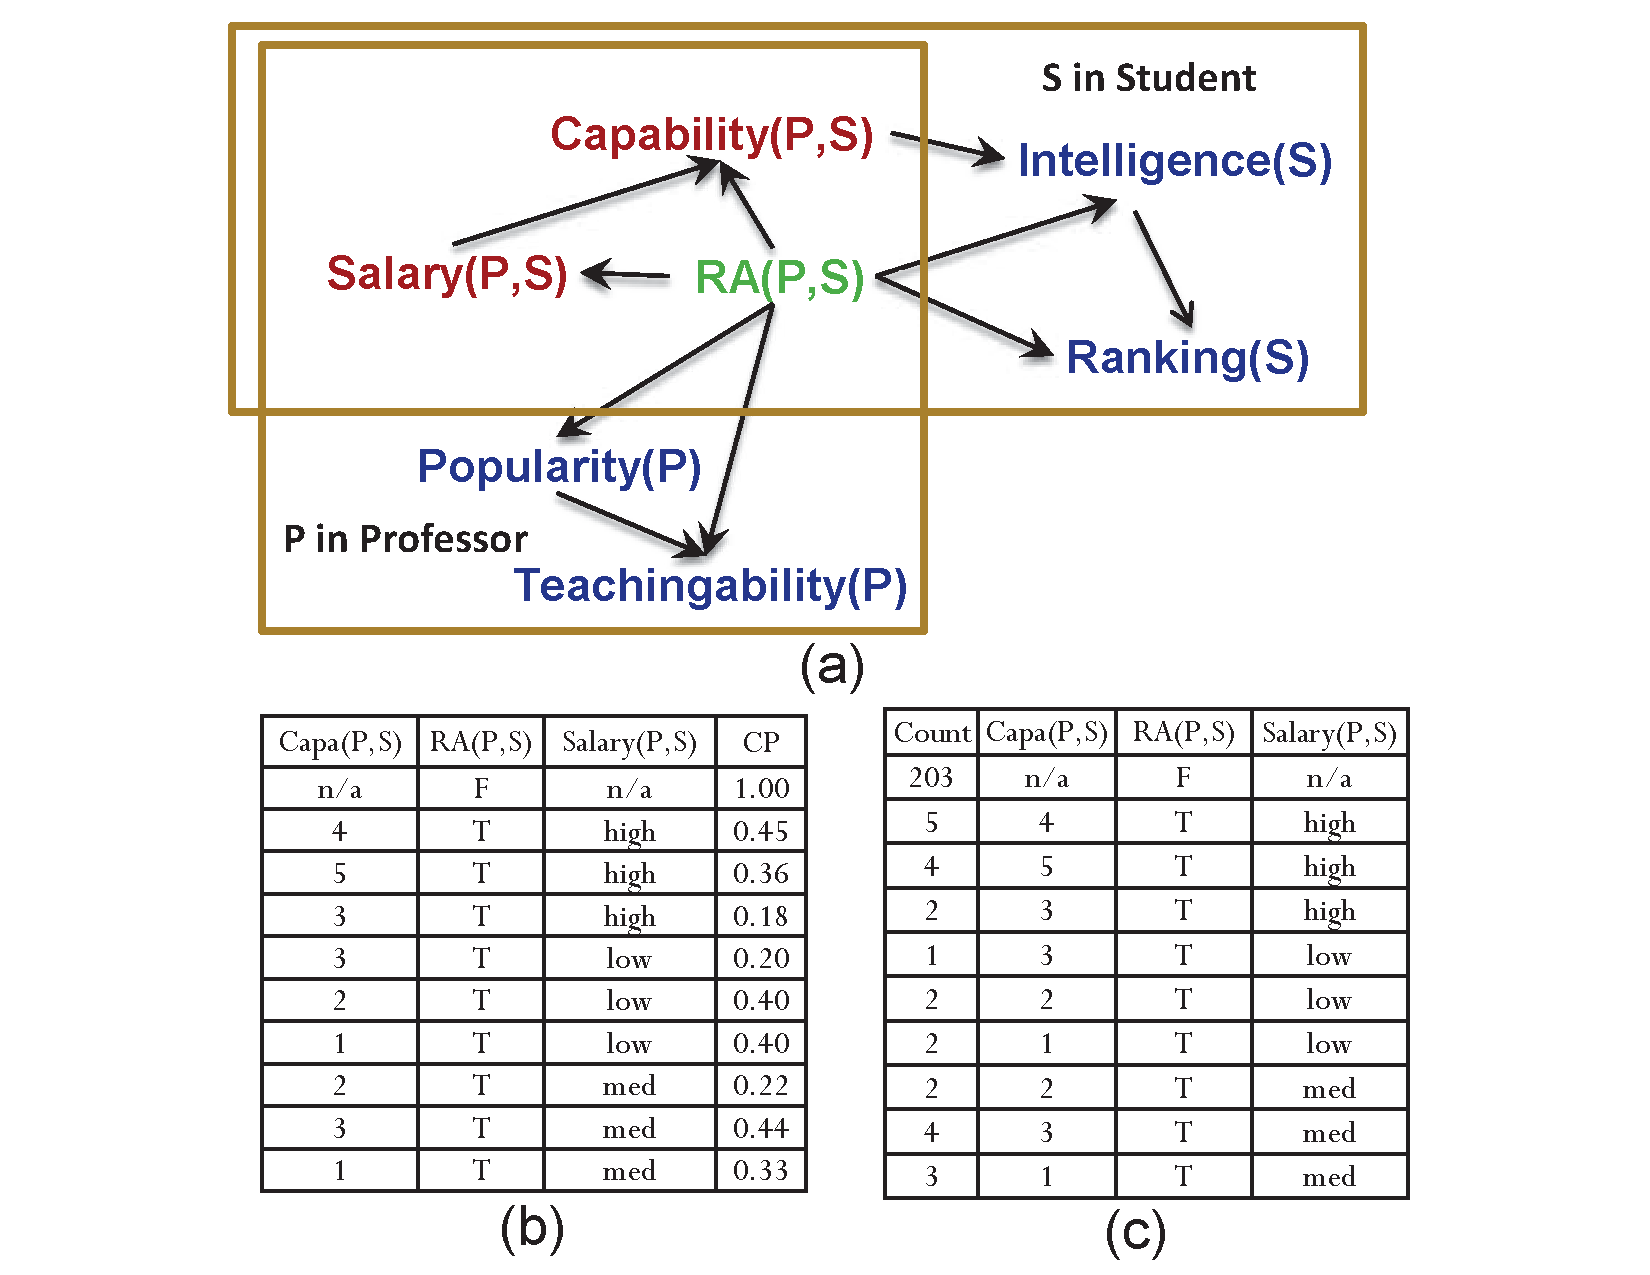
\includegraphics{pbn.pdf} 
} 
\caption{(a) Bayesian network for the University domain. I  omit the $\it{Registered}$ relationship for simplicity. The network was learned from the University dataset \cite{bib:bbsite}. (b) Conditional Probability table $Capability(\P,\S)\_\cptable$, for the node $Capability(\P,\S)$. Only value combinations that occur in the data are shown. This is an example of a factor table. (c) Contingency Table $Capability(\P,\S)\_\cttable$ for the node $Capability(\P,\S)$ and its parents. Both CP and CT tables are stored in an RDBMS.}
\label{fig:ct-cp-table1}
\end{figure}

\section{Bayes Net Learning With Link Correlation Analysis}
Constructing a Bayes Net (BN) for a relational database is very challenging. For single-table data, Bayes Net learning has been considered as a benchmark application for precomputing sufficient statistics \cite{Moore1998,lv2012}. 
Given an assignment of values to its parameters, a Bayes Net represents a joint distribution over both attributes and relationships in a relational database. 

To learn correlations between link types, I  need to provide the Bayes net with data about when links are present {\em and} when they are absent. 
FactorBase extends the previously existing learn-and-join method (LAJ), which is the state-of-the-art for Bayes net learning in relational databases \cite{Schulte2012} to support the analysis with link uncertainty. The LAJ method takes as input a contingency table for the entire database, so I  can apply it with both \textbf{link analysis on} and \textbf{link analysis off} to obtain two different BN structures for each database. 

The experiment in section \ref{sec:eva} is the first evaluation of the LAJ method with link analysis on. I use the LAJ implementation provided by system FactorBase. I  score all learned graph structures using the same full contingency table with link analysis on, so that the scores are comparable. The idea is that turning link analysis on should lead to a different structure that represents correlations, involving relationship variables, that exist in the data.

\begin{figure}[!h]
\begin{center}
\resizebox{1\textwidth}{!}{
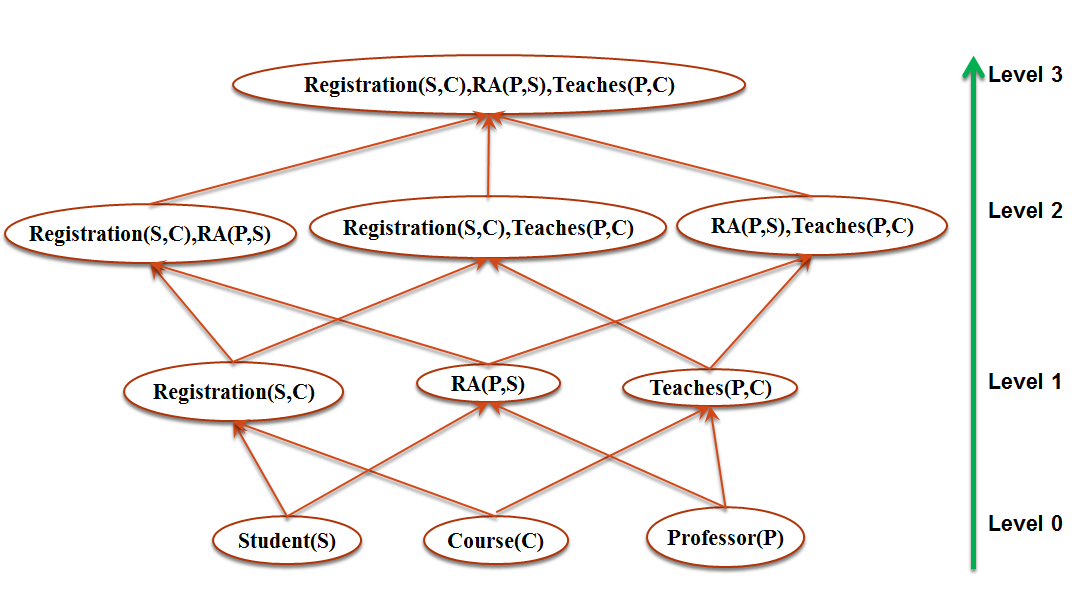
\includegraphics[width=0.9\textwidth]{unilattice.png}
}
\caption{A lattice of relationship sets for the university schema of Figure~\ref{fig:university-schema}. The arrows indicate the direction of edge propagation from lower level to upper level. \label{fig:big-lattice1}
}
\end{center}
\end{figure}


\subsection{Hierarchical Search: learn-and-join method (LAJ)}\label{sec:laj}
The key idea of the LAJ algorithm can be explained in terms of the \textbf{table join lattice} illustrated in Figure \ref{fig:big-lattice1}\footnote{Repeat the Figure \ref{fig:big-lattice} for easy review.}. 
The user chooses a single-table Bayes net learner. The learner is applied to table joins of size 1, that is, regular data tables. Then the learner is applied to table joins of size $s,s+1,\ldots$, with the constraint that larger join tables inherit the absence or presence of learned edges from smaller join tables. These edge constraints are implemented by keeping a global cache of forbidden and required edges.  


Recall that the (natural) join of two or more tables, written $\dtable_{1} \Join \dtable_{2} \cdots \Join \dtable_{k}$ is a new table that contains the rows in the Cartesian products of the tables whose values match on common fields. A table join corresponds to logical conjunction \cite{Ullman1982}.
Say that a join table $\jtable$ is a \textbf{subjoin} of another join table $\jtable'$ if $\jtable' = \jtable \Join \jtable^{*}$ for some join table $\jtable^{*}$. If $\jtable$ is a subjoin of $\jtable'$, then the fields (columns) of $\jtable$ are a subset of those in $\jtable'$. The subjoin relation defines the table join lattice. 
The moral of the learn-and-join algorithm is that join tables should inherit edges between descriptive attributes from their subjoins. This gives rise to the following constraints for two attributes $\node_{1}$, $\node_{2}$ that are both contained in some subjoin of $\jtable$. 
\begin{enumerate}
\item $\node_{1}$ and $\node_{2}$ are adjacent in a BN $B_{\jtable}$ for $\jtable$ if and only if they are adjacent in a BN for some subjoin of $\jtable$. 
\item if all subjoin BNs of $\jtable$ orient the link as $\node_{1}\rightarrow\node_{2}$ resp. $\node_{1}\leftarrow\node_{2}$, then $B_{\jtable}$ orients the link as $\node_{1}\rightarrow\node_{2}$ resp. $\node_{1}\leftarrow\node_{2}$.
\end{enumerate}
%For instance, in the University domain, if the $Student$ Bayes net contains an edge  $$intelligence(S)\rightarrow ranking(S),$$ 
%the Bayes net associated with the relationship (e.g., $Regeistration(S,C)$, $RA(P,S)$) must also contain this edge. If this edge is absent in the $Student$ Bayes net, it must also be absent in the Bayes net associated with the relationship.
Algorithm~\ref{alg:structure} provides pseudocode for the previous learn-and-join algorithm (LAJ) \cite{Schulte2012c}.

{\em Examples.} 
Consider the lattice shown in Figure~\ref{fig:big-lattice1}. 
Suppose that the Bayes net associated with the relationship $\reg(\S,\C)$ contains an edge $$\it{difficulty}(\C) \rightarrow \it{intelligence}(\S).$$ 
Then the edge $\it{difficulty}(\C) \rightarrow \it{intelligence}(\S)$ must be present in the Bayes net associated with the larger relationship set $\reg(\S,\C)$, $\it{Teaches}(\P,\C)$. If the edge is contained  in neither of the graphs associated with $\reg(\S,\C)$, and $\it{Teaches}(\P,\C)$, it must not be present in the graph associated with the $\reg(\S,\C)$, $\it{Teaches}(\P,\C)$.

\paragraph{Schema Invariance.}
The same data set may be represented under different ER schemas for various reasons, such as efficiency, data quality, and usability.
Some relational learning algorithms tend to vary quite substantially over the choice of schema, which complicates their off-the-shelf application~\cite{Picado2016}.  I circumvent the limitations of classical likelihood measures by using a relational pseudo-likelihood measure for Bayes nets \cite{Schulte2011}. 
%The pseudo log-likelihood is the expected log-likelihood of a random instantiation of the first-order variables in the PBN.
The pseudo likelihood is equivalent to an expression defined in terms of a single (hyper) population has the important consequence that it is invariant under syntactic equivalence transformations of the database. For instance, database normalization operations may move information about a descriptive attribute from one table to another \cite{Kent1983}.  Thus, the objective function of the struture learning algorithm shown in Algorithm~\ref{alg:structure} is schema invariant.



\begin{algorithm}[!h]
\begin{algorithmic}
{\footnotesize
\STATE {\em Input}: Database $\D$ with $E_1,..E_e$ entity tables, $R_1,... R_r$ Relationship tables, %ER Model ,
\STATE {\em Output}: Bayes Net for $\D$ 
\STATE {\em Calls}: PBN: Any propositional Bayes net learner that accepts edge constraints and a single table of cases as input. 
\STATE {\em Notation}: PBN$(\T,\mbox{Econstraints})$ denotes the output DAG of PBN. Get-Constraints$(\G)$ specifies a new set of edge constraints, namely that all edges in $\G$ are required, and edges missing between variables in $\G$ are forbidden.
} %fnsize
\end{algorithmic}
\begin{algorithmic}[1]
{\footnotesize
  \STATE Add descriptive attributes of all entity and relationship tables as variables to  $G$. Add a boolean indicator for each relationship table to $G$.
  \STATE Econstraints = $\emptyset$ {[Required and Forbidden edges]} %in the G]}
\FOR {m=1 to e}
  \STATE Econstraints += Get-Constraints(PBN($E_m$ , $\emptyset$)) 
  \ENDFOR 
%\FOR {m=1 to r}
% \STATE Econstraints += Get-Constraints(PBN($R_m$, Econstraints))
%\ENDFOR
\FOR {m=1 to r}
  \STATE $N_m$ :=  {\em natural join} of $R_m$ and entity tables linked to $R_m$ 
  \STATE Econstraints += Get-Constraints(PBN($N_m$, Econstraints))
\ENDFOR
\FORALL{$N_i$ and $N_j$ with a foreign key in common}
  \STATE $K_{ij}$ :=  %natural 
  join of $N_i$ and $N_j$ 
  \STATE Econstraints += Get-Constraints(PBN($K_{ij}$, Econstraints))
\ENDFOR
\RETURN Bayes Net defined by Econstraints.
    }
\end{algorithmic}
\caption{Pseudocode for previous Learn-and-Join Structure Learning for Lattice Search. \label{alg:structure}}
\end{algorithm}

%give an example to explain how LAJ works ?

\subsection {Extend LAJ for Multiple Links}\label{sec:exlaj}

To extend the learn-and-join algorithm for multiple link analysis, I replace the natural join in line 7 by the extended join (more precisely, by the contingency table derived from both positive relationship and negative relationship computed in section \ref{sec:nag}). 
The natural join contains only tuples that appear in all relationship tables. Compared to the joint contingency table, this corresponds to considering only rows where the par-Var (I also refer such as link indicator) have the value \textbf{$\true$} (e.g. RA($\P$,$\S$) = $\true$).

When the propositional Bayes net learner is applied to such a table, the link indicator variable appears like a constant. Therefore the BN learner cannot find any correlations between the link indicator variable and other nodes, nor can it find correlations among attributes conditional on the link indicator variable being $\false$. Thus the previous LAJ algorithm finds only correlations between entity attributes conditional on the existence of a relationship. In sum, hierarchical search with link correlations can be described as follows.
\begin{enumerate}
\item Run the previous LAJ algorithm (Algorithm~\ref{alg:structure}) using natural joins.
\item Starting with the constraints from step 1, run the LAJ algorithm where joint contingency table replace natural joins. That is, for each relationship set shown in the lattice of Figure~\ref{fig:big-lattice1}, apply the single-table Bayes net learner to joint contingency table for the relationship set.
\end{enumerate}



\section{Evaluation} \label{sec:eva}
I used the same FactorBase system configurations with previous chapters. For the parameter learning of the PBN, I utilize the Parameter Manager in section \ref{sec:parameters}. I also make the standard assumption that the database is complete \cite{Domingos2009,Khot2011}: For each individual (node) observed, the database lists its attributes, and for each pair of observed individuals (nodes), the database specifies which links hold between them. As of the single-table Bayes Net learner, I  made use of the following implementation:  GES search \cite{Chickering2003} with the BDeu score as implemented in version 4.3.9-0 of CMU's Tetrad package (structure prior uniform, ESS=10; \cite{2008a}).

I  used seven benchmark real-world databases as shown in Table \ref{table:datasetsize1}. For detailed descriptions and  the sources of the databases, please refer to Table~\ref{table:datasetsize} in section \ref{sec:data}. 
I  compared the following settings utilizing different setting: 
\begin{enumerate}
\item The extended LAJ method with link correlations off (Algorithm~\ref{alg:structure} utilizing  natural joins). 
\item The extended LAJ method that has the potential to find link correlations (Algorithm~\ref{alg:structure} utilizing join contingency tables). 
\end{enumerate}
\begin{table}[!h] \centering\caption{Datasets characteristics.\\ \#Tuples = total number of tuples over all tables in the dataset. 
  \label{table:datasetsize1}}
\resizebox{1\textwidth}{!}{
\begin{tabular}[c]
{|l|c|c|r|c|}\hline
 \textbf{Dataset} & \textbf{\begin{tabular}[l] {ll} \#Relationship \\Tables/ Total \end {tabular}} & \textbf{\begin{tabular}[l] {ll} \#Self \\Relationships\end {tabular}}  & \textbf{\#Tuples} & \textbf{\#Attributes}  \\\hline
    Movielens &1 / 3 & 0  & 1,010,051 & 7\\\hline
    Mutagenesis & 2 / 4 & 0 & 14,540 & 11\\\hline
    Financial &3 / 7 & 0  &  225,932& 15\\\hline
   Hepatitis &3 / 7 & 0 &12,927  & 19\\\hline
   IMDb &3 / 7 & 0 &1,354,134  & 17\\\hline
    Mondial &2 / 4 & \textbf{1} &  870& 18\\\hline
    UW-CSE &2 / 4 & \textbf{2}  & 712 & 14\\\hline   
\end{tabular}
}
\end{table}



\subsection{Structure Learning Times} 
Table~\ref{table:runtimes} provides the model search time for structure learning with link analysis on and off. Given the sufficient statistics structure learning is fast, even for the largest contingency table  IMDb (less than 10 minutes run-time). With link analysis on, structure learning takes more time as it processes more information. 
As expected in both modes, the run-time for building the contingency tables (refer to the Table~\ref{table:cttimes} in section \ref{sec:jct}) dominates the structure learning cost. For the Mondial database, there is no case where all relationship variables are simultaneously true, so with link analysis off the contingency table is empty.

\begin{table}[!h] \centering
\caption{Model Structure Learning Time  in seconds.  %N.T. = nontermination.
 \label{table:runtimes}}
\resizebox{1\textwidth}{!}{
\begin{tabular}[c]
{|l|R{4cm}|R{4cm}|}\hline
 \textbf{Dataset}  & \textbf{Link Analysis On } & \textbf{Link Analysis Off } \\\hline
Movielens & 1.53&1.44 \\\hline
Mutagenesis & 1.78&1.96 \\\hline
Financial  &96.31& 3.19 \\\hline
Hepatitis   & 416.70& 3.49\\\hline
IMDb   & 551.64 & 26.16 \\\hline
Mondial & 190.16&N/A\\\hline
UW-CSE & 2.89&2.47 \\\hline
\end{tabular}
} 

\end{table}



\subsection{Statistical Scores}
I  report two model metrics, the log-likelihood score, and the model complexity as measured by the number of parameters. The \textbf{log-likelihood} is denoted as $L(\hat{G},\d)$ where $\hat{G}$ is the BN $\G$ with its parameters instantiated to be the maximum likelihood estimates given the dataset $\d$, and the quantity $L(\hat{G},\d)$ is the log-likelihood of $\hat{G}$ on $\d$. 
I  use the relational log-likelihood score defined in \cite{Schulte2011}, which differs from the standard single-table Bayes net  likelihood only by replacing counts by frequencies  so that scores are comparable across different nodes and databases. To provide information about the qualitative graph structure learned, I  report edges learned that point to a relationship variable as a child. Such edges can be learned only with link analysis on. I  distinguish edges that link relationship variables---R2R---and that link attribute variables to relationships---A2R. For instance, in the most intuitive Financial dataset, there are two R2R edges and nine A2R edges, as shown in Figure \ref{fig:finbn}.
And for the IMDb dataset, eleven A2R edges were captured in the learned BN struture with link analysis on which is shown in Figure \ref{fig:imdbbn}.

\begin{figure}[H]	
\begin{center}
\resizebox{1\textwidth}{!}{
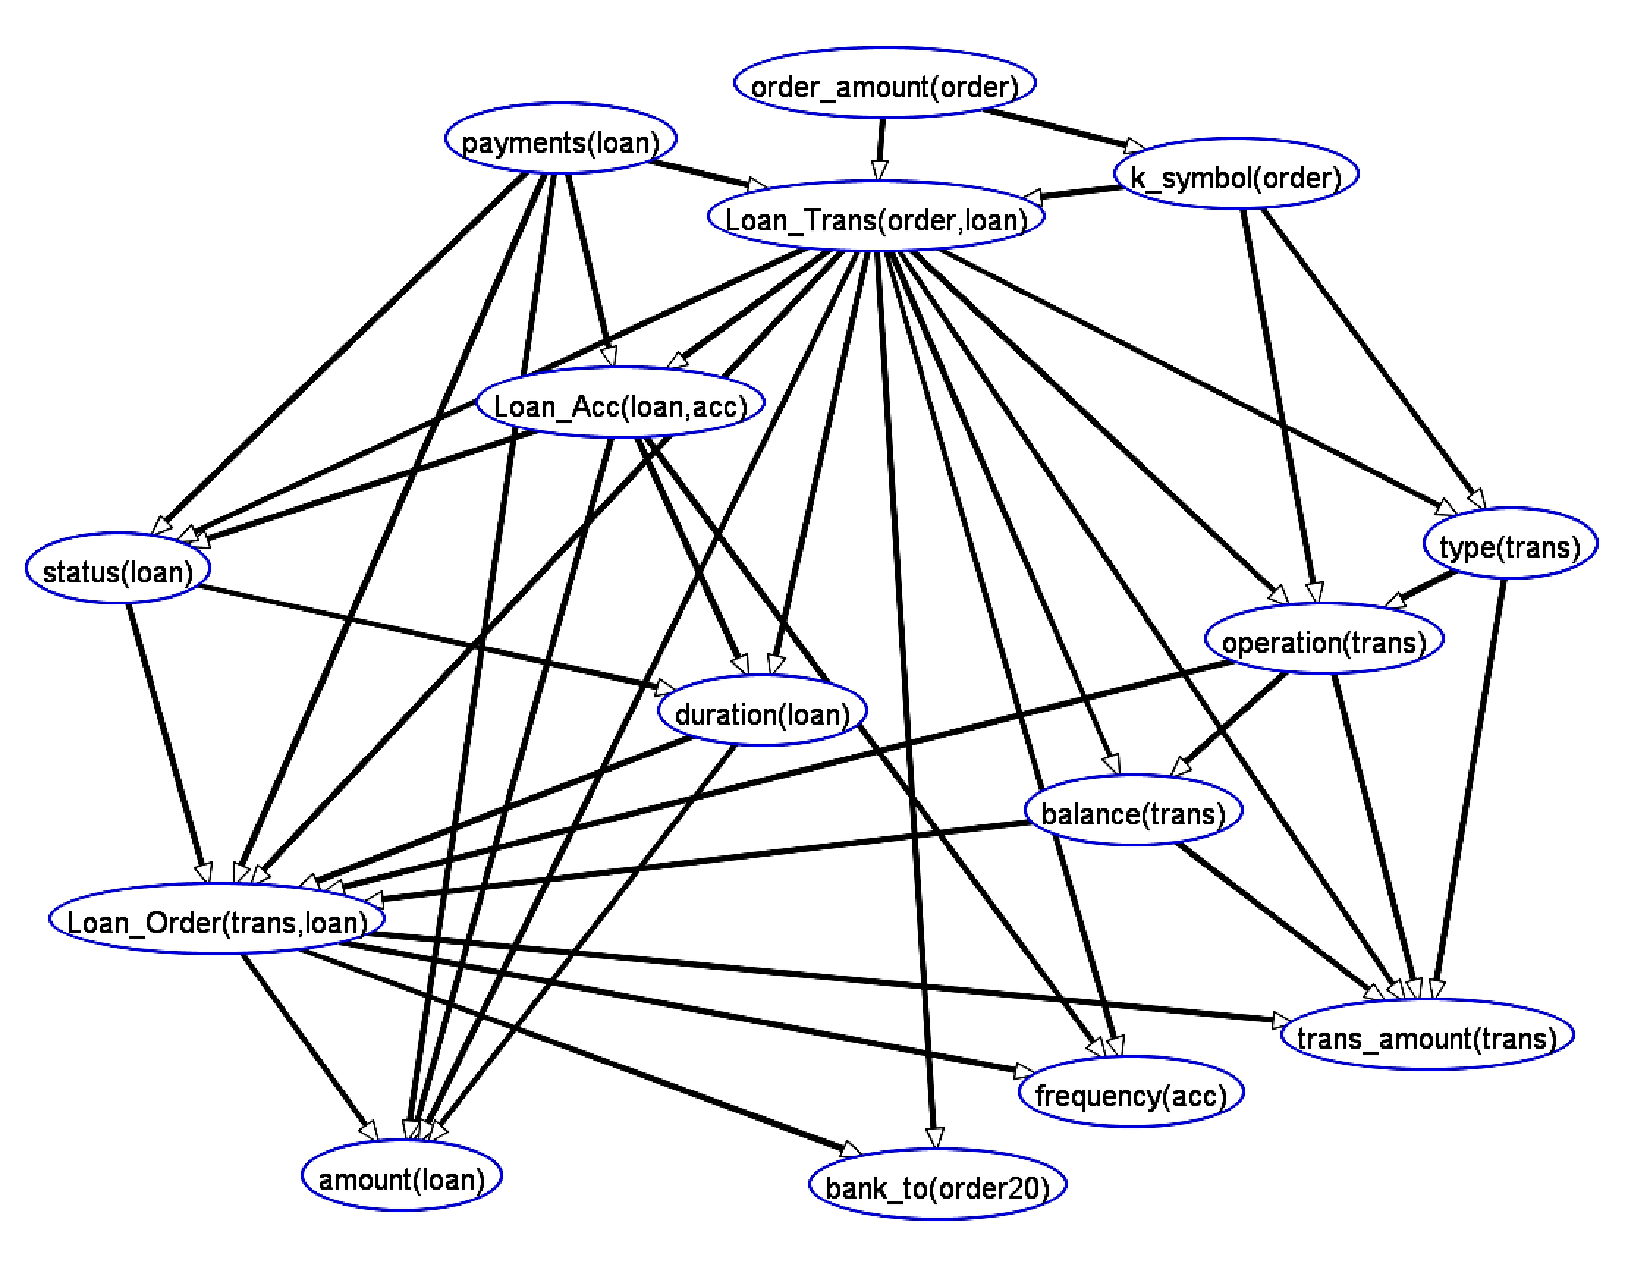
\includegraphics[width=0.9\textwidth]{financialBN}
}
\caption{The learned Bayes Net for Financial dataset with link analysis on.\label{fig:finbn}
}
\end{center}
\end{figure}
\begin{figure}[H]
\begin{center}
\resizebox{1\textwidth}{!}{
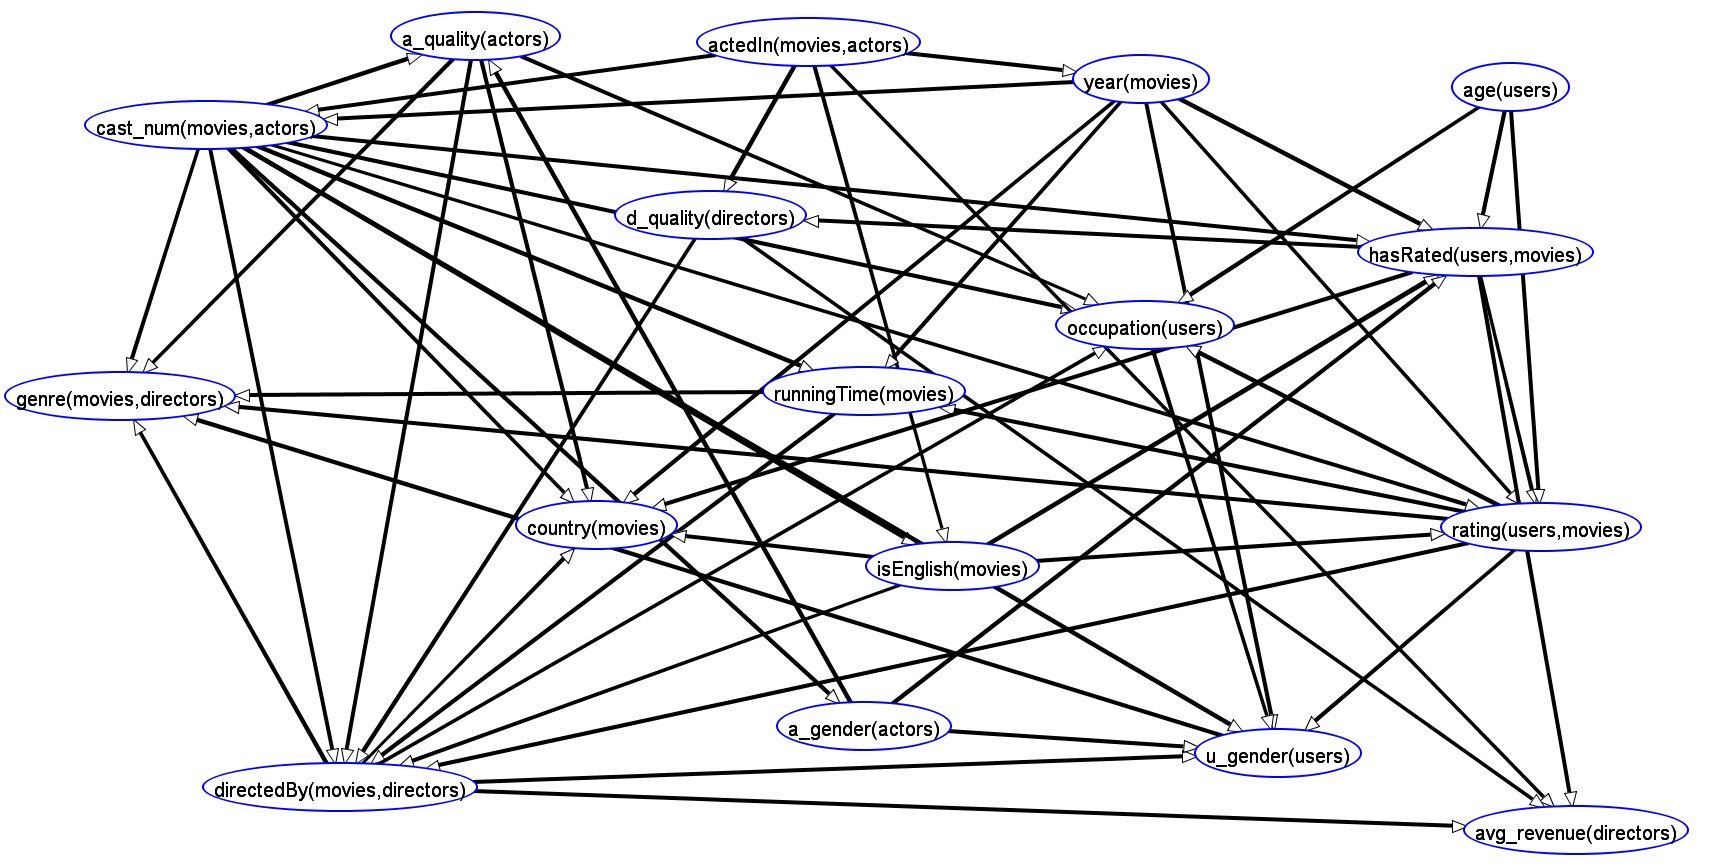
\includegraphics[width=0.9\textwidth]{imdbBN}
}
\caption{The learned Bayes Net for IMDb dataset with link analysis on.\label{fig:imdbbn}
}
\end{center}
\end{figure}


Structure learning can use the new type of dependencies to find a better, or at least different, trade-off between model complexity and model fit.
On two datasets (IMDb and Financial), link analysis leads to a superior model that achieves better data fit with fewer parameters. These are also the datasets with the most complex relational schemas (see Table~\ref{table:datasetsize1}). On IMDb in particular, considering only positive links leads to a very poor structure with a huge number of parameters.
On four datasets, extra sufficient statistics lead to different trade-offs: On MovieLens and Mutagenesis, link analysis leads to better data fit but higher model complexity, and the reverse for Hepatitis and UW-CSE. 

\begin{table}[h] 
\begin{center}
\caption{Comparison of Statistical Performance of Bayesian Network Learning.
}
\resizebox{1 \textwidth}{!}{
\begin{tabular}{|m{3cm}|R{3cm}|R{3cm}|R{1cm}|R{1cm}| }
\hline \textbf{Movielens } &{log-likelihood} &{\#Parameter}& {R2R}&{A2R}\\
\hline
Link Analysis Off    & -4.68 & \textbf{164} & 0     & 0 \\
\hline
Link Analysis On  & \textbf{-3.44} & 292   & 0     & 3 \\
\hline
%Complete & -3.44 & 675   & 0     & 0 \\
%\hline
%Disconnected & -4.31 & 15    & 0     & 0 \\
%\hline
    \end{tabular}
}
\end{center}

\begin{center}
\resizebox{1 \textwidth}{!}{
\begin{tabular}{|m{3cm}|R{3cm}|R{3cm}|R{1cm}|R{1cm}| }\hline 
\textbf{Mutagenesis } &{log-likelihood} &{\#Parameter}& {R2R}&{A2R}\\  \hline 
Link Analysis  Off   & -6.18 & \textbf{499} & 0     & 0 \\ \hline
Link Analysis  On  & \textbf{-5.96} & 721   & 1     & 5  \\ \hline
%Complete & -5.59 & 423,369 & 1     & 0 \\ \hline
%Disconnected & -7.91 & 36    & 0     & 0 \\ \hline
    \end{tabular}
}
\end{center}
%Financial
\begin{center}
\resizebox{1 \textwidth}{!}{
\begin{tabular}{|m{3cm}|R{3cm}|R{3cm}|R{1cm}|R{1cm}| }
\hline \textbf{Financial } &{log-likelihood} &{\#Parameter}& {R2R}&{A2R}\\    \hline
Link Analysis Off   & -10.96 & 11,572 & 0     & 0 \\ \hline
Link Analysis On  & \textbf{-10.74} & \textbf{2433} & 2     & 9 \\ \hline
%Complete & -10.67 & 374,399,999 & 3     & 0 \\ \hline
%Disconnected & -12.79 & 49    & 0     & 0 \\ \hline
    \end{tabular}
}
\end{center}  

\begin{center}
\resizebox{1 \textwidth}{!}{
\begin{tabular}{|m{3cm}|R{3cm}|R{3cm}|R{1cm}|R{1cm}| }
\hline \textbf{Hepatitis  } &{log-likelihood} &{\#Parameter}& {R2R}&{A2R}\\   \hline
Link Analysis Off   & \textbf{-15.61} & 962   & 0     & 0 \\      \hline
Link Analysis On  & -16.58 & \textbf{569} & 3     & 6 \\      \hline
%Complete & NT    & NT    & 3     & 0 \\      \hline
%Disconnected & -18.30 & 58    & 0     & 0 \\     \hline
    \end{tabular}
}
\end{center}

\begin{center}
\resizebox{1 \textwidth}{!}{
\begin{tabular}{|m{3cm}|R{3cm}|R{3cm}|R{1cm}|R{1cm}| }
\hline \textbf{IMDb  } &{log-likelihood} &{\#Parameter}& {R2R}&{A2R}\\    \hline
Link Analysis Off    & -13.63 & 181,896 & 0     & 0 \\    \hline
Link Analysis On  & \textbf{-11.39} & \textbf{60,059} & 0     & 11 \\     \hline
%Complete & N.T.   & N.T.    & 3     & 0 \\     \hline
%Disconnected & -12.01 & 54    & 0     & 0 \\   \hline
    \end{tabular}
}
\end{center}

\begin{center}
\resizebox{1 \textwidth}{!}{
\begin{tabular}{|m{3cm}|R{3cm}|R{3cm}|R{1cm}|R{1cm}| }
\hline \textbf{Mondial  } &{log-likelihood} &{\#Parameter}& {R2R}&{A2R}\\   \hline
Link Analysis Off   &   N/A    &  N/A     & N/A     & N/A \\    \hline
Link Analysis On& -18.2 & 339   & 0     & 4 \\    \hline
%Complete & N.T.    & N.T.    &     3  & 0 \\     \hline
%Disconnected & -19.98 & 55    & 0     & 0 \\   \hline
    \end{tabular}
}
\end{center}

\begin{center}
\resizebox{1 \textwidth}{!}{
\begin{tabular}{|m{3cm}|R{3cm}|R{3cm}|R{1cm}|R{1cm}| }
\hline \textbf{UW-CSE   } &{log-likelihood} &{\#Parameter}& {R2R}&{A2R}\\   \hline
Link Analysis Off   & \textbf{-6.68} & 305   & 0     & 0 \\  \hline
Link Analysis On & -8.13 & \textbf{241} & 0     & 2 \\  \hline
%Complete & -6.02 & 22,118,399 & 3     & 0 \\  \hline
%Disconnected & -10.24 & 45    & 0     & 0 \\ \hline
    \end{tabular}
}
\end{center}

\label{table:result_scores}
\end{table}

%show link-on BNs, consistant with the results? 


\section{Conclusion} 
The model described in this chapter captures a wider class of correlations that involve uncertainty about the link structure. 
I  extend the state-of-the-art algorithm for learning correlations among link types and node attributes in relational data that represent complex heterogeneous network with many attributes and link types. The link correlations are represented in a Bayes net structure. This provides a succinct graphical way to display relational statistical patterns and support powerful probabilistic inferences. Statistical measures indicate that Bayes net methods succeed in finding relevant correlations. 




\chapter{Instance Level Learning of Relational Dependency Networks} \label{cha:RDN}


Learning graphical models is one of the main approaches to extending machine learning for relational data. Two major classes of graphical models are Bayesian networks (BNs) \cite{Pearl1988}  and dependency networks (DNs)~\cite{Heckerman2000}. In chapter \ref{cha:lbn}, I discussed the generative modeling with Bayes net by learning a model of the joint probability distribution of all input random variables. Dependency networks are well suited for the task of discriminative predicting preferences such as classification problem to predict the label $y$ given all inputs $x$.

In this chapter, I describe a new approach for instance level dependency networks learning: first learn a Bayes net, then convert that network to a dependency network. This hybrid approach combines the speed of learning Bayes net with the advantages of dependency network inference for relational data. The experiments show that the hybrid learning algorithm can produce dependency networks for large and complex databases, up to one million records and 19 predicates. The predictive accuracy of the resulting networks is competitive with those from state-of-the-art function gradient boosting methods
but scales substantially better than the boosting methods.
%
\section{Introduction}
%\subsection{Motivation.}
The hybrid approach combines different strengths of Bayesian networks and dependency networks for relational learning. The special strength of Bayesian networks is scalability in learning~\cite[Sec.8.5.1]{Neville2007},\cite{Khosravi2010}. Bayesian networks offer closed-form parameter estimation via the maximum likelihood method, and therefore closed-form model evaluation. Model evaluation is the computationally most expensive part of relational learning, as it requires combining information from different related tables, which involves expensive table joins. 


\begin{figure}[!h]
\begin{center}
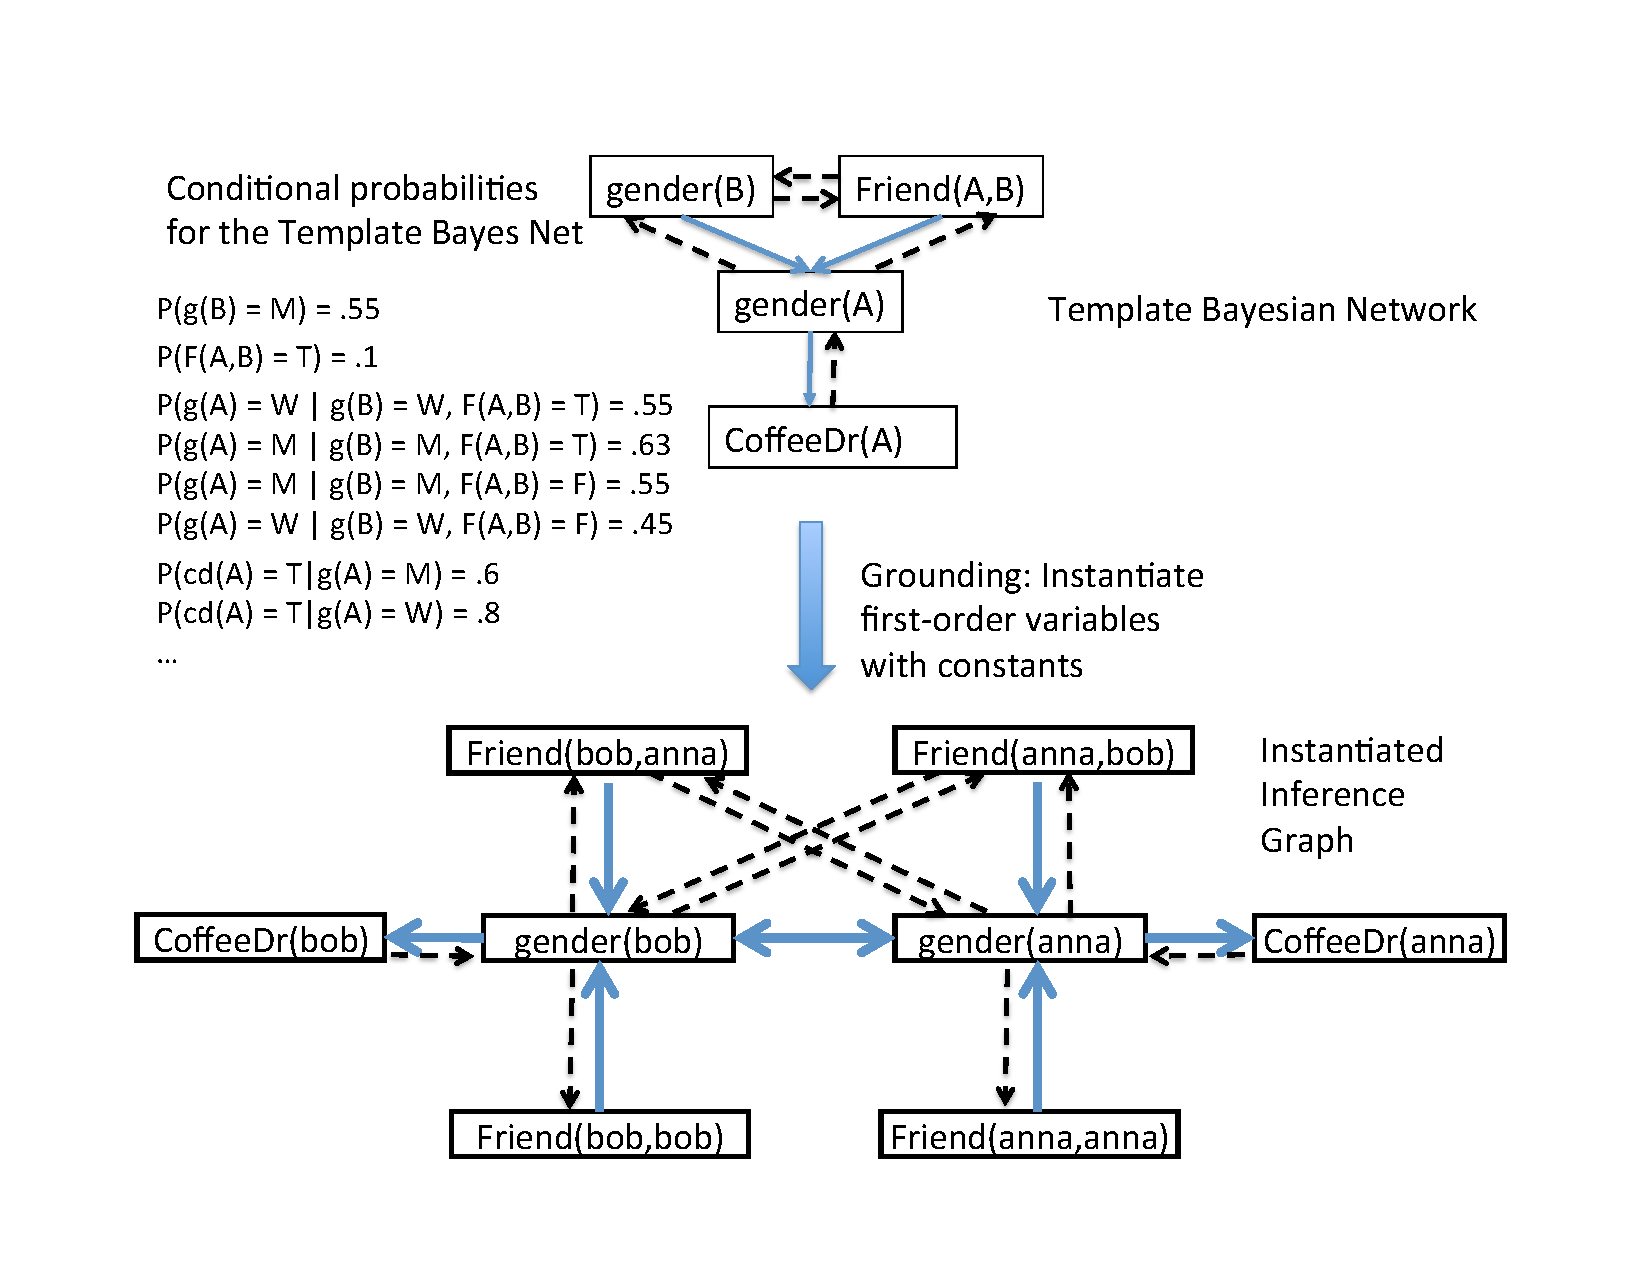
\includegraphics[width = 1 \textwidth]{dn.pdf}
\caption{A Bayesian/dependency template network (top) and the instantiated inference graphs (bottom). By convention, predicates (Boolean functors) are capitalized. Edges from the BN template are solid blue, while edges added by the BN-to-DN transformation are dashed black. The edge set in the DN comprises both solid and dashed arrows. Note that although the template BN (top) is acyclic, its  instantiation (bottom) features a bi-directed edge between $\it{gender}(bob)$ and $\it{gender}(anna)$. \label{fig:dn}
}
\end{center}
\end{figure} 
In contrast, a strength of relational dependency networks is that they support inference in the presence of cyclic dependencies\cite{Neville2007,Natarajan2012}. Cyclic dependencies occur when a relational dataset features auto-correlations, where the value of an attribute for an individual depends on the values of the same attribute for related individuals. Figure~\ref{fig:dn}  provides an example. It is difficult for Bayesian networks to model auto-correlations because by definition, the graph structure of a Bayesian network must be acyclic \cite{Domingos2007,Taskar2002,Getoorprm2001}. Because of the importance of relational auto-correlations, dependency networks have gained popularity since they support reasoning about cyclic dependencies using a directed graphical model. 

These advantages  of the hybrid approach are specific to relational data. For propositional (\iid) data, which can be represented in a single table, there is no problem with cyclic dependencies, and the acyclic constraint of Bayesian networks can actually make probabilistic inference more efficient \cite{Hulten2003}. Also, the closed-form model evaluation of Bayesian networks is relatively less important in the single-table case, because iterating over the rows of a single data table to evaluate a dependency network is relatively fast compared to iterating over ground atoms in the relational case, where they are stored across several tables. 

My approach extends the moralization approach to relational structure learning, which learns an undirected Markov model by first learning a Bayesian network structure, then converts the network structure to a Markov logic structure, without parameters \cite{Khosravi2010,Schulte2012}. That approach also combines the scalable learning of Bayesian networks with the support undirected models offer for inference with auto-correlation. 
%(which do not contain cycles since their graphs are undirected). 
The present work extends this by also computing the dependency network parameters from the learned Bayesian network. The previous work used only the Bayesian network structure. The theoretical analysis shows that the learned dependency networks provide different predictions from Markov networks. 

\paragraph{Contributions}

I  make three main contributions:
\begin{enumerate}
\item A faster approach for learning relational dependency networks: first learn a Bayesian network, then convert it to a dependency network.
\item A closed-form log-linear discriminative model for computing the relational dependency network parameters from Bayesian network structure and parameters.
\item Necessary and sufficient conditions for the resulting network to be \defterm{consistent}, defined as the existence of a single joint distribution that induces all the conditional distributions defined by the dependency network \cite{Heckerman2000}.
\end{enumerate}




\section{Bayesian Networks and Relational Dependency Networks} 
I  review dependency networks and their advantages for modelling relational data. I assume familiarity with the basic concepts of Bayesian networks \cite{Pearl1988}. 
 
 \subsection{Dependency networks and Bayesian networks} 
The structures of both Bayesian networks and dependency networks are defined by a directed graph whose nodes are random variables. Bayesian networks must be acyclic, while dependency networks may contain cycles, including the special case of bi-directed edges. For both networks, the parameters are conditional distributions over the value of a node given its parents. The two types differ in the  influence of a node's children, however. In a Bayesian network, a node is only independent of all other nodes given an assignment of values to its parents, its children, and the co-parents of its children, whereas in a dependency network a node is independent given an assignment of values to only its parents. In graphical model terms, the \defterm{Markov blanket} of a node in a dependency network, the minimal set of nodes such that assigning them values will make this node independent of the rest of the network, is simply its parents.\footnote{For this reason Hofmann and Tresp originally used the term ``Markov blanket networks'' for dependency networks~\cite{Hofmann1998}.}
For a Bayesian network, the Markov blanket is the node's parents, children, and the co-parents of its children.

Consequently, a conditional probability in a dependency network effectively specifies the probability of a node value given an assignment of values to {\em all} other nodes. 
Following Heckerman \etal{}~\cite{Heckerman2000}, I  refer to such conditional probabilities as \defterm{local probability distributions}.


\subsection{Relational Dependency Networks}\label{sec:rdns}


As described in section \ref{sec:log-linear}, I  present the relational case using the parametrized random variable notation~\cite{Kimmig2015}.
Relational dependency networks~\cite{Neville2007} extend dependency networks to model distributions over multiple populations.
A functor is a symbol denoting a function or predicate. Each functor has a set of values (constants) called the \defterm{domain} of the functor. Functors with boolean ranges are called \textbf{predicates} and their name is capitalized. I  consider only functors with finite domains. An expression $\functor(\term_{1},\ldots,\term_{k})$, where $\functor$ is a functor and each $\term_{i}$ is a first-order variable or a constant, is a \defterm{Parametrized Random Variable} (PRV).
 
A directed acyclic graph whose nodes are PRVs is a \defterm{parametrized Bayesian network structure}, while a general (potentially cyclic) directed graph whose nodes are PRVs is a \defterm{relational dependency network structure} (RDN). A Bayesian network structure or relational dependency network structure augmented with the appropriate conditional probabilities is  respectively a \defterm{Bayesian network template} or \defterm{relational dependency network template}.  Note that the RDN templates that I  define in this chapter have the same Markov blanket as the Bayesian network templates from which they are derived but a different edge structure and probabilities. Algorithm~\ref{alg:dnfeatures}, defined in Section~\ref{sect:learning}, converts the probabilities of the Bayesian template to their counterparts in the relational dependency template. 

\begin{algorithm}[!h]
%\linesnumbered
\SetKwData{Calls}{Calls}
\SetKwData{Notation}{Notation}
%\begin{algorithmic}
%{\footnotesize
%\STATE {\em Input}: Database $\D$ with $\etable_1,..\etable_e$ entity tables, functors $\F$, variable number bound $\varbound$.
\KwIn{Template Bayesian Network $\BN$ (Structure and Parameters)}
\KwOut{A List of Relevant Features; a Weight for each Feature }
\begin{algorithmic}[1]
\FOR{ each target node $\TT$}
\STATE{initialize $\it{Feature\_Weight}\_\it{List}(\TT)$ as the empty list}
	\FOR{ each $\UT$ in $\{ \Setaddterm{\TT} {\Ch{\TT}}\}$}
	\FOR {each value $\UV$ of the child node $\UT$ }
		\FOR {each vector of parent values $ \Prange{\UT}$}
			\STATE $\it{Feature}$ $F$  $:=$ $(\Appendterm{\UT  = \UV} {\Pa{\UT} = \Prange{\UT}})$ 
			\STATE  $\it{FeatureWeight} $ $\weight:=$ $\ln\cprob{\UT = \UV}{\Pa{\UT} = \Prange{\UT}}$
			\IF{the Feature $F$ does not contain a false relationship other than $\TT$}%, i.e. not relevant in $\BN$}
				\STATE{ add $(F , \weight)$ to $\it{Feature\_Weight}\_\it{List}(\TT)$  }
			\ENDIF \\	
		\ENDFOR
	\ENDFOR
\ENDFOR 
\ENDFOR
\STATE \Return {$\it{Feature\_Weight}\_\it{List}(\TT)$}
	%\STATE \Return $\Relfreq{C}{\DB}:=$ $\Relcount{C}{\DB}/\it{Total\_Relevant\_Count}$.
\end{algorithmic}
%\label{alg:cpt}
\caption{Computing Features and Weights for Template Dependency Network. \label{alg:dnfeatures}}
\end{algorithm}


RDNs extend dependency networks from \iid{} to relational data via knowledge-based model construction \cite{Neville2007}:
The first-order variables in a template RDN graph are instantiated for a specific domain of individuals to produce an {\em  instantiated} or {\em ground} propositional DN graph, the \defterm{inference graph}. Figure~\ref{fig:dn} gives a dependency network template and its  inference graph. Given an edge in the template RDN, instantiating both the parent and the child of the edge with the same grounding produces an edge in the inference graph. An example local probability distribution for the graph in Figure~\ref{fig:dn} (abbreviating functors) is
$$P(\it{g(anna)}|\it{g(bob)}, \it{CD(anna)}, \it{F(anna,bob)},\it{F(bob,anna)},\it{F(anna,anna)}).$$

\paragraph{Language Bias.}
The general definition of a parametrized random variable allows PRVs to contain constants as well as population variables. Another language extension is to allow parametrized random variables to be formed with aggregate functions, as described by Kersting and deRaedt \cite{Kersting2007}. For example, it is possible to use a functor that returns the number of friends of a generic person $\A$. The main contribution of this paper, the relational BN-to-DN conversion method, can be used whether the parametrized random variables contain constants, aggregates, or only first-order variables. A common restriction to simplify model structure learning is to exclude constants (e.g. \cite{Friedman99prm,Domingos2009}). 

Friedman {\em et al.} investigated learning directed graphical models with aggregate functions \cite{Friedman99prm}. 





\section{Learning Relational Dependency Networks via Bayesian Networks}\label{sect:learning}
\begin{figure}[!h]
\begin{center}
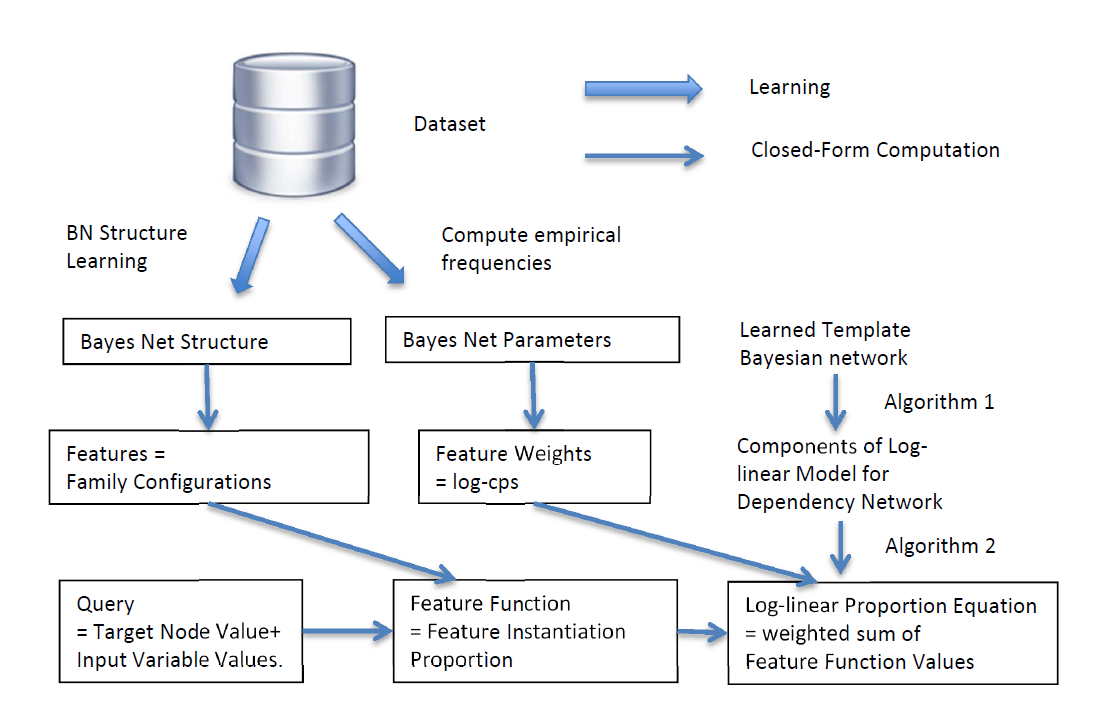
\includegraphics[width=1\textwidth]{bn-regress.png}
\caption{The program flow for computing local probability distributions from a template Bayesian network. Features and weights are computed from the Bayesian network. Feature function values are computed for each query. \label{fig:bn-flow}}
\end{center}
\end{figure}
The algorithm for rapidly learning relational dependency networks (Figure~\ref{fig:bn-flow}) begins with any relational learning algorithm for Bayesian networks. Using the resulting Bayesian network as a template, I  then apply a simple, fast transformation to obtain a relational dependency template. Finally I  apply a closed-form computation to derive the dependency network inference graph parameters from the Bayesian structure and parameters. 


\subsection{BN-to-DN structure conversion}
Converting a Bayesian network structure to a dependency network structure is simple: for each node, add an edge pointing to the node from each member of its BN Markov blanket~\cite{Heckerman2000}.  The result contains  bidirectional links between each node, its children, and its co-parents (nodes that share a child with this one). 

This is equivalent to the standard moralization  method for converting a BN to an undirected model \cite{Domingos2009}, except that the dependency network contains bi-directed edges instead of undirected edges. Bidirected edges have the advantage that they permit  assignment of different parameters to each direction, whereas undirected edges have only one parameter. 


\subsection{BN-to-DN parameter conversion}  
For propositional data, converting Bayesian network parameters to dependency network parameters is simple: apply the standard BN product formula and solve for the local probability distributions given Bayesian network parameters~\cite[Ch.14.5.2]{Russell2010}. A \defterm{family} comprises a node and its parents. A \defterm{family configuration} specifies a value for a child node and each of its parents. For example, in the template of Figure~\ref{fig:dn}~(top), one family is $\it{gender}(\A), \it{Friend}(\A,\B), \it{gender}(\B)$ and one of its eight possible configurations is
$$\it{gender}(\A) = \Man, \it{Friend}(\A,\B) = \true, \it{gender}(\B) = \Man.$$
The Markov blanket of a target node comprises multiple families, one each for the target node and each of its children, so
an assignment of values to the target's Markov blanket defines a unique configuration for each family. Hence in the propositional case the Markov blanket induces a {\em unique} log-conditional probability for each family configuration. The probability of a target node value given an assignment of values to the Markov blanket is then proportional to {\em the exponentiated sum of these log-conditional probabilities} \cite[Ch.14.5.2]{Russell2010}.

With relational data, however, different family configurations can be simultaneously instantiated, {\em multiple times.}  I  generalize the propositional log-linear equation for relational data by replacing the unique log-conditional probability with the {\em expected} log-conditional probability that results from selecting an instantiation of the family configuration uniformly at random. The probability of a target node value given an assignment of values to the Markov blanket is then proportional to the exponentiated sum of the expected log-conditional probabilities. %Without this normalization, features with more instantiations carry exponentially more weight. 
I  describe the resulting closed-form equation in the next section. 


\section{The Log-linear Proportion Equation} \label{sec:theequation}

I  propose a log-linear equation, the \defterm{log-linear proportion equation} (lower right box of Figure~\ref{fig:bn-flow}), for computing a local probability distribution for a ground target node, $\FG{\TT}$, given (i) a target value $\TV$ for the target node, (ii) a complete set of values $\QC$  for all ground terms other than the target node, and (iii) a template Bayesian network. The template structure is represented by functions that return the set of parent nodes of $\UT$, $\Pa{\UT}$, and the set of child nodes of $\UT$, $\Ch{\UT}$. The parameters of the template are
represented by the conditional probabilities of a node $\UT$ having a value $\UV$ conditional on the values of its parents, $\cprob{\UT = \UV}{\Pa{\UT} = \Prange{\UT}}$. A grounding $\grounding$ substitutes a constant for each member of a list of first-order variables, $\{\A_{1} = \a_{1},\ldots, \A_{k} = \a_{k}\}$. Applying a grounding to a template node defines a fully ground target node: $\it{gender}(\A) \{\A = sam\} = \it{gender}(sam)$.  These are combined in the following log-linear equation to produce a local probability distribution:

%
\begin{definition}[The Log-Linear Proportion Equation]\label{def:log-diff-freq-eq}
\begin{eqnarray*}
  \Gprob{\FG{{\TT}} = \TV} {\QC} &\propto &  \exp\\
 \sum_{\UT} \sum_{\UV,\Prange{\UT}}   \quad \left[ \ln \cprob{\UT = \UV}{\Pa{\UT} = \Prange{\UT}} \right] &
    \cdot &
    \Relfreq{\Appendterm{\grounding;\UT  = \UV} {\Pa{\UT} = \Prange{\UT}}} {\Qconj}
%    \Relfreq{\Appendterm{\Ground{\UI}  = \UV} {\Ground{\Pa{\UI}} = \Prange{\UT}}} {\Qconj}
\end{eqnarray*}
where 
\begin{eqnarray*}
%\UT &\mbox{varies over} &  \TT \mbox{and its children}; \\
\UT &\mathrm{varies\ over} & \Setaddterm{\{\TT\}} {\Ch{\TT}}; \\
\mbox{the singleton value} \ \UV & \mathrm{varies\ over} & \mbox{the range of}\  \UT;\\
\mbox{the vector of values} \ \Prange{\UT} & \mathrm{varies\ over} & \mbox{the product of the ranges of} \ \UT's\ \mbox{parents}, \\
& & \mbox{constrained to value} \ \TV \ \mbox{for occurrences of} \ \TT;\\
\FG{\TT} = \TT \grounding&\mathrm{is} & \mbox{is the target grounding of template node }  \TT; \\
\mbox{and}~\Relevant{\Fvar} &\mathrm{is} & \mbox{the feature function, the family proportion}.
\end{eqnarray*}
\end{definition}

The family proportion $\Relevant{\Fvar}$ is computed as follows:
%In terms of log-linear models, this corresponds to using family configurations as features and the {\em proportion of instantiations} that satisfy a family configuration as the feature function. 
\begin{enumerate}
\item For a given family configuration $(\Appendterm{\UT  = \UV} {\Pa{\UT} = \Prange{\UT}})$, let the \defterm{family  count} $$\Count{\Appendterm{\grounding;\UT  = \UV} {\Pa{\UT} = \Prange{\UT}}} {\Qconj}$$ be the number of instantiations that (a) satisfy the family configuration and the ground node values specified by $\Qconj$, and (b) are consistent with the equality constraint defined by the grounding $\grounding$.
%This notation is consistent with the parfactor notation of \cite{Poole2003}. 
\item The \defterm{relevant family count} $n^{r}$ is 0 if the family configuration contains a false relationship (other than the target node), else equals the family count. It is common in statistical-relational models to restrict predictors to existing relationships only \cite{Getoor2007c,Russell2010}.
\item The \defterm{family proportion} is the relevant family count, divided by the total sum of all relevant family counts for the given family:
{\scriptsize
\begin{equation} \notag
 \Relfreq{\Appendterm{\grounding;\UT  = \UV} {\Pa{\UT} = \Prange{\UT}}} {\Qconj} = \frac{\Relcount{\Appendterm{\grounding;\UT  = \UV} {\Pa{\UT} = \Prange{\UT}}} {\Qconj}}{\sum_{\UV',\Prange{\UT}'}\Relcount{\Appendterm{\grounding;\UT  = \UV'} {\Pa{\UT} = \Prange{\UT}'}} {\Qconj}}
\end{equation}
}
\end{enumerate}

In the experiments, family counts and proportions are computed using exact counting methods (see Section~\ref{sec:complexity} below).


\subsection{Example and Pseudocode}
Table~\ref{table:log-diff-example} illustrates the computation of these quantities for predicting the gender of a new test instance ($sam$). Algorithm~\ref{alg:dnfeatures} shows pseudocode for the closed-form transformation of Bayesian network structure and parameters into features and weights for the dependency network. Algorithm~\ref{alg:log-linear} shows pseudocode for computing the scores defined by the log-linear Equation~\eqref{def:log-diff-freq-eq}, given a list of weighted features and a target query. 


\begin{algorithm}[!h]
%\linesnumbered
\SetKwData{Calls}{Calls}
\SetKwData{Notation}{Notation}
%\begin{algorithmic}
%{\footnotesize
%\STATE {\em Input}: Database $\D$ with $\etable_1,..\etable_e$ entity tables, functors $\F$, variable number bound $\varbound$.
\KwIn{Feature-Weight List of Dependency Network, Query $ \Gprob{\FG{{\TT}} = \TV} {\QC}=?$. $\TT$ is a template node, $\FG{\TT} = \TT \grounding$ is the target grounding. }
%Feature $F = \Appendterm{\Ground{\UI}  = \UV} {\Ground{\Pa{\UI}} = \Prange{\UT}}$}
\KwOut{Normalized log-linear score}
\begin{algorithmic}[1]
%\FOR{ each target node $\TT$}
\STATE{initialize $\it{score}(\FG\TT = \TV) :=$ 0}
%\STATE{initialize $\it{score}_{\grounding} (\FG\TT) :=$ 0}
%\STATE $\Gprob{\FG{{\TT}} = \TV} {\QC} :=$ 0
%\FOR{ each $\UT$ in $\{ \Setaddterm{\FG\TT} {\Ch{\FG\TT}}\}$}
%\FOR {each vector of parent values $ \Prange{\UT}$}
\FOR {each Feature $F = (\Appendterm{\UT  = \UV} {\Pa{\UT} = \Prange{\UT}})$ in  $\it{Feature\_Weight}\_\it{List}(
\TT)$}
% \COMMENT{compute feature function}}%%	\IF{the feature $F$ is not relevant in $\BN$}
%\STATE $\it{Feature}$ $F$  $:=$ $(\Appendterm{\UT  = \UV} {\Pa{\UT} = \Prange{\UT}})$ 
%	\STATE  $\it{FeatureWeight} $ $\weight:=$ $\ln\cprob{\UT = \UV}{\Pa{\UT} = \Prange{\UT}}$
%	\IF{the Feature $F$ does not contain a false relationship other than $\TT$}%, i.e. not relevant in $\BN$}
%	\STATE $\it{RelFamCnt} :=$ $ 0$ 
%	\ELSE
\STATE  Let $\weight $ be the weight listed for feature $F$ 
\STATE \COMMENT{Next compute feature function.}
	\STATE   $\it{RelFamCnt}(F)$ $ :=$ $\Relcount{{\grounding}; \Appendterm{{\UI}  = \UV} {{\Pa{\UI}} = \Prange{\UT}}} {\Qconj}$
	\STATE $\it{TotalRelFamCnt}(U)$ := $\sum_{\UV',\Prange{\UT}'}\Relcount{ {\grounding}; \Appendterm{{\UI}  = \UV'} {{\Pa{\UI}} = \Prange{\UT}'}} {\Qconj}$
	\STATE  $\it{Family Proportion }$ $ \Relevant{\Fvar}(F) :=$ $\it{RelFamCnt}(F)/\it{TotalRelFamCnt}(U)$ \\
	%\COMMENT{$\it{FamilyProportion}$ is $\Relfreq{{\grounding}; \Appendterm{\Ground{\UI}  = \UV} {\Ground{\Pa{\UI}} = \Prange{\UT}}} {\Qconj}$ }
%	\STATE  $\it{Family Proportion}\cdot  \it{FeatureWeight}$
	\STATE   $\it{score}(\FG\TT = \TV)$ $\mathrel{+}= \Relevant{\Fvar}  \cdot  \weight $
%	\STATE{ add $(F , \weight)$ to $\it{Feature}\_\it{List}(\TT)$  }
%	\ENDIF \\
	%\STATE	
%\ENDFOR
\ENDFOR
%\ENDFOR
%\ENDFOR 
\STATE \Return {Normalized scores for target node.}
	%\STATE \Return $\Relfreq{C}{\DB}:=$ $\Relcount{C}{\DB}/\it{Total\_Relevant\_Count}$.
\end{algorithmic}
%\label{alg:cpt}
\caption{Computing local probability distributions, the parameters of the Inference  Dependency Network. %\textbf{make notation consistent with ILP, not JAIR.} %Feature =  Family Configuration. 
\label{alg:log-linear}}
\end{algorithm}

\begin{table}[tb]
\caption{Applying the log-linear proportion equation with the Bayesian network of Figure~\ref{fig:dn} to compute $\Gprob{\it{gender}(sam) = \Woman} {\QC}$ and $\Gprob{\it{gender}(sam) = \Man} {\QC}$. Each row represents a feature/family configuration. For the sake of the example I  suppose that the conjunction $\QC$ specifies that Sam is a coffee drinker, has 60 male friends, and 40 female friends. $CP$ is the conditional probability BN parameter of Figure~\ref{fig:dn} and $\weight \equiv \ln(CP)$.
\label{table:log-diff-example}}
\centering
%\resizebox{1.1\textwidth}{!}{
\begin{tabular}{l@{\hspace{.2in}}l@{\hspace{.1in}}r@{\hspace{.1in}}r@{\hspace{.1in}}r@{\hspace{.1in}}r}
% This is a hand-computed example. 
{\setlength{\tabcolsep}{0pt}\begin{tabular}{l}Child \\Value $\UV$ \end{tabular}}&Parent State $\Prange{\UT}$&CP 
%$\cprob{\UT = \UV}{\Pa{\UT} = \Prange{\UT}}$
&{\setlength{\tabcolsep}{0pt}\begin{tabular}{c} $w$ \end{tabular}}&$\Relevant{\Fvar}$&{\setlength{\tabcolsep}{0pt}\begin{tabular}{c} $w \times \Relevant{\Fvar}$ \end{tabular}} \\\hline
$g(sam) = \Woman$&{\setlength{\tabcolsep}{0pt}\begin{tabular}{l}$ g(B) = \Woman,$\\ $F(sam,B) = \true$\end{tabular}}&$0.55$&$-0.60$&$0.4$&$-0.24$ \\
$g(sam) = \Woman$&{\setlength{\tabcolsep}{0pt}\begin{tabular}{l}$ g(B) = \Man,$\\ $ F(sam,B) = \true$\end{tabular}}&$0.37$&$-0.99$&$0.6$&$-0.60$ \\
$CD(sam) = \true$&{\setlength{\tabcolsep}{0pt}\begin{tabular}{l}$ g(sam) = \Woman$\end{tabular}}&$0.80$&$-0.22$&$1.0$&$-0.22$ \\
$CD(sam) = \false$&{\setlength{\tabcolsep}{0pt}\begin{tabular}{l}$g(sam) = \Woman$ \end{tabular}}&$0.20$&$-1.61$&$0.0$&$0.00$ \\\hline
\multicolumn{5}{l}{Sum ($\exp(Sum) \propto\Gprob{gender(sam)=\mathrm{\Woman}}{\QC}$)}&$-1.06$ \\\hline
$g(sam) = \Man$&{\setlength{\tabcolsep}{0pt}\begin{tabular}{l}$ g(B) = \Woman,$\\ $F(sam,B) = \true$\end{tabular}}&$0.45$&$-0.80$&$0.4$&$-0.32$ \\
$g(sam) = \Man$&{\setlength{\tabcolsep}{0pt}\begin{tabular}{l}$ g(B) = \Man,$\\ $ F(sam,B) = \true$\end{tabular}}&$0.63$&$-0.46$&$0.6$&$-0.28$ \\
$CD(sam) = \true$&{\setlength{\tabcolsep}{0pt}\begin{tabular}{l}$ g(sam) = \Man$\end{tabular}}&$0.60$&$-0.51$&$1.0$&$-0.51$ \\
$CD(sam) = \false$&{\setlength{\tabcolsep}{0pt}\begin{tabular}{l}$ g(sam) = \Man$\end{tabular}}&$0.40$&$-0.92$&$0.0$&$0.00$ \\\hline
\multicolumn{5}{l}{Sum ($\exp(Sum) \propto\Gprob{gender(sam)=\mathrm{\Man}}{\QC}$)}&$-1.11$ \\\hline

\end{tabular}
%}
\end{table}

%It is common in statistical-relational models to restrict predictors to existing relationships only \cite{Getoor2007c,Russell2010}.

The inner sum of Equation~\eqref{def:log-diff-freq-eq} computes the expected log-conditional probability for a family with child node $\UT$, when I  randomly select a relevant grounding of the first-order variables in the family.


\subsection{Discussion and Motivation} 

I  discuss the key properties of the local distribution model, Equation~\eqref{def:log-diff-freq-eq}. 

\paragraph{Log-Linearity.} The survey by Kimmig {\em et al.} \cite{Kimmig2015} shows that most statistical-relational methods define log-linear models. The general form of a discriminative log-linear model \cite{Sutton2007} is that the conditional probability of a target variable value given input variable values is proportional to an exponentiated weighted sum of feature functions. A feature function maps a complete assignment of ground node values (= target value + input variables) to a real number. Khazemi {\em et al.} have shown that many relational aggregators can be represented by a log-linear model with suitable features \cite{Kazemi2014}. 
Equation~\eqref{def:log-diff-freq-eq} instantiates this well-established log-linear schema as follows: The features of the model are the family configurations $(\Appendterm{\UT  = \UV} {\Pa{\UT} = \Prange{\UT}})$ 
%that specify the values of a child node and its parents in the template Bayesian network, 
where the child node is either the target node or one of its children. The feature weights are the log-conditional BN probabilities defined for the family configuration. The input variables are the values specified for the ground (non-target) nodes by the conjunction $\QC$.
%The family count specifies how many times the feature is instantiated in the input variables (plus the target node value).
The feature functions are the family proportion $\Relevant{\Fvar}$. Like other log-linear relational models, Equation~\ref{def:log-diff-freq-eq} enforces parameter tying, where different groundings of the same family configuration receive the same weight~\cite{Kimmig2015}. 

\paragraph{Standardization.} Using proportions as feature functions has the desirable consequence that the range of all feature functions is standardized to [0,1]. It is well-known that the number of instantiation counts in relational data can differ for different families, depending on the population variables they contain. This ill-conditioning causes difficulties for log-linear models because families with more population variables can have an exponentially higher impact on the score prediction \cite{Lowd2007}. Intuitively, counts tacitly conflate number of instantiations with degree of information. Proportions avoid such ill-conditioning.

\paragraph{Generalizing the Propositional Case.} A useful general design principle is that relational learning should have propositional learning as a special case~\cite{Ch.10deraedt,Knobbe2006}: When I  apply a relational model to a single \iid{} data table, it should give the same result as the propositional model. Equation~\ref{def:log-diff-freq-eq} satisfies this principle. In the propositional case, an assignment of values to all nodes other than the target node specifies a {\em unique} value for each family configuration. This means that all the family counts $n^{r}$ are either 0 or 1, hence all relevant proportions $p^{r}$ are 0 or 1, depending on whether a family configuration matches the query or not. For a simple illustration, consider the edge $\it{gender}(\A) \rightarrow \it{CoffeeDr}(\A)$. Since this edge concerns only the $\it{Person}$ domain associated with the single population variable $\A$, I  may 
view this edge as a propositional subnetwork.
%
%the structure $\it{gender} \rightarrow \it{CoffeeDr}$ as a propositional subnetwork. 
Suppose the query is $P(\it{gender}(sam)= \Woman|\it{CoffeeDr}(sam)=\true)$. The only family configurations with nonzero counts are $\it{gender}(sam)= \Woman$ (count 1) and $\it{CoffeeDr}(sam)=\true),\it{gender}(sam)= \Woman$ (count 1). Equation~\eqref{def:log-diff-freq-eq} gives
\begin{eqnarray*}
P(\it{g}(sam)= \Woman|\it{CD}(sam)=\true) \propto \\
\exp \{\ln P(\it{g}(sam)= \Woman) + \ln P(\it{CD}(sam)=\true)|\it{g}(sam)= \Woman)\}.&&
\end{eqnarray*}

%$\Relcount$

This agrees with the propositional BN formula for a local conditional probability, which is the product of the BN conditional probabilities for the target node given its children, and the target node's children given their parents. This formula can be derived from the BN product rule for defining a joint probability \cite[Ch.14.5.2]{Russell2010}. In the simple two-node example, it can be derived immediately from Bayes' theorem:
\begin{eqnarray*}
P(\it{g}(sam)= \Woman|\it{CD}(sam)=\true) \propto \\
P(\it{CD}(sam)=\true)|\it{g}(sam)= \Woman) \times P(\it{g}(sam)= \Woman),&&
\end{eqnarray*}

\noindent which agrees with the solution above derived from Equation~\eqref{def:log-diff-freq-eq}. It may seem surprising that in predicting gender given coffee drinking, the model should use the conditional probability of coffee drinking given gender. However, Bayes' theorem states that $P(X|Y)$ is proportional to $P(Y|X)$. In the example, given that the BN model specifies that women are more likely to be coffee drinkers than men, the information that Sam is a coffee drinker raises the probability that Sam is a woman. 

\subsection{Complexity of Algorithms \ref{alg:dnfeatures} and \ref{alg:log-linear}} \label{sec:complexity}
%\paragraph{Computing Features and Feature Weights} 
The loops of Algorithm~\ref{alg:dnfeatures} enumerate every family configuration in the template Bayesian network exactly once. Therefore {\em computing features and weights takes time linear in the number of parameters of the Bayesian network.} 

Evaluating the log-linear equation, as shown in Algorithm~\ref{alg:log-linear}, requires finding the number of instantiations that satisfy a conjunctive family formula, given a grounding. This is an instance of the general problem of computing the number of instantiations of a formula in a relational structure. Computing this number is a well-studied problem  with highly efficient solutions \cite{Vardi1995,Schulte2014}. 

A key parameter is the number $m$ of first-order variables that appear in the formula. A loose upper bound on the complexity of counting instantiations is $d^{m}$, where $d$ is the maximum size of the domain of the first-order variables. Thus counting instantiations has parametrized polynomial complexity \cite{Flum2006}, meaning that if $m$ is held constant, counting instantiations requires polynomially many operations in the size of the relational structure (i.e., the size of $\Qconj$ in Equation~\eqref{def:log-diff-freq-eq}). For varying $m$, the problem of computing the number of formula instantiations is \#P-complete \cite[Prop.12.4]{Domingos2007}.


 

\section{Consistency of the Derived Dependency Networks} \label{sec:consistency} A basic question in the theory of dependency networks is the {\em consistency} of the local probabilities.  Consistent local probabilities ensure the existence of a single joint probability distribution $p$ that induces the various local conditional probability distributions $P$ for each node
$$\Gprob{\FG{\TT} = \TV} {\QC} \propto p(\FG{\TT} =\TV,\QC)$$  
for all target nodes $\FG{\TT}$ and query conjunctions $\QC$~\cite{Heckerman2000}.

I  present a precise condition on a template Bayesian network for its resulting dependency network to be consistent and the implications of those conditions.  I  define an \defterm{edge-consistent template Bayesian network} to be a network for which every edge has the same set of population variables on both nodes.

\begin{theorem}\label{th:consistent-dn}
A template Bayesian network is edge-consistent if and only if its derived dependency network is consistent.
\end{theorem}

%

The proof of this result is complex, so I  present it in an appendix. Intuitively, in a joint distribution, the correlation or potential of an edge 
is a single fixed quantity, whereas in Equation~\eqref{def:log-diff-freq-eq}, the correlation is adjusted by the size of the relational neighbourhood  of the target node, which may be either the child or the parent of the edge. If the relational neighborhood size of the parent node is different from that of the child node, the adjustment makes the conditional distribution of the child node inconsistent with that of the parent node. The edge-consistency characterization shows that the inconsistency phenomenon is properly relational, meaning it arises when network structure contains edges that relate parents and children from different populations.



The edge-consistency condition required by this theorem is quite restrictive: Very few template Bayesian networks will have exactly the same set of population variables on both sides of each edge.\footnote{A commonly used weaker condition is range-restriction: that the population variables in the child node should be contained in the population variables of its parents \cite{Kersting2007}, but not vice versa as with edge-consistency.}
}
%
Therefore relational template Bayesian networks, which have multiple population variables, will most often produce inconsistent dependency networks. Previous work has shown that dependency networks learned from data are almost always inconsistent but nonetheless provide accurate predictions using ordered pseudo-Gibbs sampling~\cite{Heckerman2000,Neville2007,Lowd2012} or Generative Stochastic Networks \cite[Sec.3.4]{Bengio2014}.

\section{Empirical Evaluation: Design and Datasets}\label{sec:empirical-comparison}
There is no obvious baseline method for the RDN learning method because mine is the first work that uses the approach of learning an RDN via a Bayesian network. Instead I benchmark against the performance of a different approach for learning RDNs, which uses an ensemble learning approach based on functional gradient boosting. Boosted functional gradient methods have been shown to outperform previous methods for learning relational dependency networks \cite{Khot2011,Natarajan2012}. 



\paragraph{Datasets}
I used six benchmark real-world databases with the FactorBase system. Summary statistics are given in Table~\ref{table:learning-times}. For more details please see the references in \cite{Schulte2012}.
\paragraph{Methods Compared} Functional gradient boosting is a state-of-the-art method for applying discriminative learning to build a generative graphical model. The local discriminative models are  ensembles of relational regression trees \cite{Khot2011}. Functional gradient boosting for relational data is implemented in the Boostr system~\cite{Khot2013}.
 For functors with more than two possible values, I  followed \cite{Khot2011} and converted each such functor to a set of binary predicates by introducing a predicate for each possible value.

%
I  compared the following methods:
\begin{description}
\item[RDN\_Bayes] my method: Learn a Bayesian network, then convert it to a relational dependency network.
\item[RDN\_Boost] The RDN learning mode of the Boostr system \cite{Natarajan2012}. 
%Information from ground nodes linked to the target is aggregated with functions $count, max, average$ and existential quantification .
\item[MLN\_Boost] The MLN learning mode of the Boostr system. It takes a  list of target predicates for analysis. I  provide each binary predicate in turn as a single target predicate, which amounts to using MLN learning to construct an RDN. This RDN uses a log-linear model for local probability distributions that is derived from Markov Logic Networks.
\end{description}
I  used the default Boostr settings. I  experimented with alternative settings but they did not improve the performance of the boosting methods.

\paragraph{Prediction Metrics}
I  follow \cite{Khot2011} and evaluate the algorithms using conditional log likelihood (CLL) and area under the precision-recall curve (AUC-PR). AUC-PR is appropriate when the target predicates features a skewed distribution as is typically the case with relationship predicates. %These metrics have been used in previous evaluations of MLN learning~\cite{Domingos2007,Schulte2012}.  
For each fact $\FG{\TT} = \TV$ in the test dataset, I  evaluate the accuracy of the predicted local probability $\Gprob{\FG{\TT} = \TV} {\QC}$, where $\QC$ is a complete conjunction for all ground terms other than $\FG{\TT}$. Thus $\QC$ represents the values of the input variables as specified by the test dataset.
%For classification accuracy, a model's prediction is scored as correct if the true value of the ground term in the test dataset receives the highest Gibbs probability. 
CLL is the average of the logarithm of the local probability for each ground truth fact in the test dataset, averaged over all test predicates. For the gradient boosting method, I  used the AUC-PR and likelihood scoring routines included in Boostr.

Both metrics are reported as means and standard deviations over all binary predicates. The learning methods were evaluated using 5-fold cross-validation. Each database was split into 5 folds by randomly selecting entities from each entity table, and restricting the relationship tuples in each fold to those involving only the selected entities  (i.e., subgraph sampling~\cite{Schulte2012}). The models were trained on 4 of the 5 folds, then tested on the remaining one. 

\section{Results} 
%


I  report learning times and accuracy metrics. In addition to these quantitative assessments, I  inspect the learned models to compare the model structures. Finally I  make suggestions for combining the strenghts of boosting with the strengths of Bayesian network learning. 


\subsection{Learning Times} Table~\ref{table:learning-times} shows learning times for the methods. The Bayesian network  learning simultaneously learns a joint model for all parametrized random variables (PRVs). Recall that Boolean PRVs are predicates. For the boosting method, I  added together the learning times for each target PRV. 
On MovieLens(1M), the boosting methods take over 2~days to learn a classifier for the relationship $B\_U2Base$, so I  do not include learning time for this predicate for any boosting method.
On the largest database, IMDb, the boosting methods cannot learn a local distribution model for the three relationship predicates with my system resources, so I  only report learning time for descriptive attributes by the boosting methods. Likewise, the accuracy results in Tables~\ref{table:cll} and~\ref{table:AUC} include only measurements for descriptive attributes on the datasets IMDb and MovieLens(1M).
%\textbf{Cathy: need to add bold}

\begin{table}[tb]
  \addtolength{\tabcolsep}{2pt}
  \centering
  \caption{Learning Time. The total learning time for constructing a relational dependency network from an input database. Only partial boosting learning times are reported for the larger databases MovieLens(1M) and IMDb---see text for details. Spread is reported as coefficient of variation (CV---standard deviation / mean). PRV = Parametrized Random Variable.\label{table:learning-times}}
\begin{tabular}{l r r @{\hspace{20pt}} r r r r r r }\hline
             &           &             &  \multicolumn{2}{c}{RDN\_Bayes} & \multicolumn{2}{c}{RDN\_Boost} & \multicolumn{2}{c}{MLN\_Boost}\\
                                               \cline{4-5}                                  \cline{6-7}                                  \cline{8-9}
Dataset & kTuple & PRVs & (s) & CV & (s) & CV & (s) & CV \\\hline
UW & 0.6 & 14 & \textbf{14} & 0.00 & 237 & 0.06 & 329 & 0.16 \\
Mondial & 0.9 & 18 & 1836 & 0.07 & \textbf{369} & 0.06 & 717 & 0.05 \\
Hepatitis & 11.3& 19 & 5434 & 0.01 & 6648 & 0.02 & \textbf{3197} & 0.04 \\
Mutagenesis & 24.3& 11 & \textbf{11} & 0.00 & 1342 & 0.04 & 1040 & 0.02 \\
MovieLens(0.1M) & 83.4& 7 & \textbf{8} & 0.07 & 3019 & 0.04 & 3292 & 0.01 \\
MovieLens(1M) & 1010.1& 7/6 & \textbf{8} & 0.09 & 32230 & 0.04 & 25528 & 0.04 \\
IMDb & 15538.4& 17/13 & \textbf{9346} & 0.22 & 78129 & 0.04 & 29704 & 0.03 \\\hline
\end{tabular}
\end{table}

Consistent with other previous experiments on Bayesian network learning with relational data~\cite{Khosravi2010,Schulte2012}, Table~\ref{table:learning-times} shows that RDN\_Bayes scales very well with the number of data tuples: even the MovieLens dataset with 1~M records can be analyzed in seconds. 
%This is because it provides closed-form parameter estimation and hence closed-form model scoring. 
RDN\_Bayes is less scalable with the number of PRVs, since it learns a joint model over all PRVs simultaneously,  although the time  remains feasible (1--3 hours for 17--19 predicates; see also \cite{Schulte2012}). By contrast, the boosting methods scale well with the number of predicates, which is consistent with findings from  propositional learning \cite{Heckerman2000}.
%\cite{Heckerman2000,Hulten2003}.
Gradient boosting scales much worse with the number of data tuples.
 
{\addtolength{\tabcolsep}{2pt}
\begin{table}[tb]
  \centering
  \caption{Conditional Log-Likelihood: Mean (top), Std. Dev. (bottom) }
    \begin{tabular}{l r r r r r r r}
    \hline
                 &          &              &                 &          & \multicolumn{2}{c}{MovieLens} & \\
                                                                                 \cline{6-7}
    Method & UW    & Mond. & Hepa. & Muta. & (0.1M) & (1M) & IMDb \\
    \hline
    RDN\_Boost & -0.30 & -0.48 & -0.48 & -0.36  & -0.50 & \textbf{-0.22} & \textbf{-0.49} \\
    MLN\_Boost & -0.14 & -0.40 & -0.49 & -0.23 & -0.50 & -0.23 & \textbf{-0.49} \\
    RDN\_Bayes & \textbf{-0.01} & \textbf{-0.25} & \textbf{-0.39} & \textbf{-0.22} & \textbf{-0.30} & -0.28 & -0.51 \\
    \hline
    RDN\_Boost & 0.02 & 0.03 & 0.01 & 0.02 & 0.01 & 0.00 & 0.00 \\
    MLN\_Boost & 0.01 & 0.05 & 0.01 & 0.02 & 0.01 & 0.00 & 0.00 \\
    RDN\_Bayes & 0.00 & 0.06 & 0.10 & 0.07 & 0.00 & 0.00 & 0.00 \\
    \hline
    \end{tabular}%
  \label{table:cll}%
\end{table}%
}
% Table originally generated by Excel2LaTeX from sheet 'AUC-PR'
% Since modified to move standard deviations to end and improve formatting
\begin{table}[tb]
  \addtolength{\tabcolsep}{2pt}
  \centering 
  \caption{Area Under Precision-Recall Curve: Mean (top), Std. Dev. (bottom).}
    \begin{tabular}{c r r r r r r r}    \hline
                 &          &            &          &           & \multicolumn{2}{c}{MovieLens} & \\
                                                                          \cline{6-7}     
    Method & UW    & Mond. & Hepa. & Muta. & (0.1M) & (1M)                            & IMDb\\
    \hline
    RDN\_Boost &0.42&0.27&0.55&0.71&0.50&0.88&0.63 \\
    MLN\_Boost &0.68&0.44&0.55& \textbf{0.86} &0.50&0.88&0.63 \\
    RDN\_Bayes & \textbf{0.89} & \textbf{0.79} &0.55&0.50& \textbf{0.65} &\textbf{1.00}& \textbf{0.85} \\
    \hline
    RDN\_Boost &0.00&0.00&0.01&0.02&0.01&0.00&0.01 \\
    MLN\_Boost &0.01&0.04&0.01&0.04&0.01&0.00&0.01 \\
    RDN\_Bayes &0.00&0.07&0.11&0.10&0.02&0.00&0.00 \\
    \hline
    \end{tabular}%
  \label{table:AUC}%
\end{table}%
%


\subsection{Accuracy} Whereas learning times were evaluated on all PRVs, unless otherwise noted, I  evaluate accuracy on all the  binary predicates only (e.g., $\it{gender},\it{Borders}$) because the boosting methods are based on binary classification. By the conditional likelihood metric (Table~\ref{table:cll}), the Bayesian network method performs best on four datasets, comparably to MLN\_Boost on Mutagenesis, and slightly worse than both boosting methods on the two largest datasets. By the precision-recall metric (Table~\ref{table:AUC}), the Bayesian network method performs substantially better on four datasets, identically on Hepatitis, and substantially worse on Mutagenesis.

Combining these results, for most of the datasets the Bayesian network method has comparable accuracy and much faster learning. This is satisfactory because boosting is a powerful method that achieves accurate predictions by producing a tailored local model for each target predicate. By contrast, Bayesian network learning simultaneously constructs a joint model for all predicates, and uses simple maximum likelihood estimation for parameter values.
I  conclude that \emph{Bayesian network  learning scales much better to large datasets, and provides competitive accuracy in predictions.} 
 
\subsection{Comparison of Model Structures} 
Boosting is known to lead to very accurate classification models in general \cite{Bishop2006}. For propositional data, a Bayesian network classifier with maximum likelihood estimation for parameter values is a reasonable baseline method \cite{Grossman2004}, but I  would expect less accuracy than from a boosted ensemble of regression trees.
Therefore the predictive performance of the RDN models is not due to the log-linear equation~\eqref{def:log-diff-freq-eq}, but due to the \textbf{more powerful features} that Bayesian network learning finds in relational datasets. These features involve longer chains of relationships than I observe in the boosting models.\footnote{Kok and Domingos emphasize the importance of learning clauses with long relationship chains \cite{Kok2010}.} 
The ability to find complex patterns involving longer relationship chains comes from the lattice search strategy, which in turn depends on the scalability of model evaluation in order to explore a complex space of relationship chains. Table~\ref{table:mb-comparison} reports results that quantitatively confirm this analysis.
 
\begin{table}[!htbp]
 \addtolength{\tabcolsep}{5pt}
 \caption{Difference in Markov blankets between RDN\_Bayes and RDN\_Boost. $\Delta x$ = ($x$ for RDN\_Bayes - $x$ for RDN\_Boost).  RDN\_Bayes predicts a target more successfully because it uses more  predicates and those predicates contain more first-order variables.}
      \centering
\begin{tabular}{l l c c c c}
\hline
Database & Target & $\Delta$ Predicates  & $\Delta$ Vars. & $\Delta$ CLL & $\Delta$ AUC-PR \\\hline
Mondial & religion & 11 & 1 & 0.58 & 0.30\\
%IMDb & gender & 6 & 2 & 0.3 & 0.68 \\
IMDb & gender & 4 & 2 & 0.30 & 0.68 \\
UW-CSE & student & 4 & 1 & 0.50 & 0.55 \\
Hepatitis & sex & 4 & 2 & 0.20 & 0.25\\
Mutagenesis & ind1 & 5 & 1 & 0.56 & 0.22 \\
MovieLens & gender & 1 & 1 & 0.26 & 0.26 \\\hline
\end{tabular}
 \label{table:mb-comparison}%
\end{table}% 


For each database, I  selected the target PRV where RDN-Bayes shows the greatest predictive advantage over RDN-Boost (shown as $\Delta$ CLL and $\Delta$ AUC-PR). I  then compute how many more PRVs the RDN-Bayes model uses to predict the target predicate than the RDN-Boost model, shown as $\Delta$ Predicates. This number can be as high as 11 more PRVs (for Mondial). I  also compare how many more population variables are contained in the Markov blanket of the RDN-Bayes model, shown as $\Delta$ Variables. In terms of database tables, the number of population variables measures how many related tables are used for prediction in addition to the target table. This number can be as high as 2 (for IMDb and Hepatitis). To illustrate Figure~\ref{fig:dn-structure} shows the parents (Markov blanket) of target node $\it{gender}(\U)$ from IMDb in the RDN-Boost and RDN-Bayes models. The RDN-Bayes model introduces 4 more parents and 2 more variables, $\it{Movie}$ and $\it{Actor}$. These two variables correspond to a relationship chain of length 2. Thus BN learning discovers that the gender of a user can be predicted by the gender of actors that appear in movies that the user has rated.

\begin{figure}[H]
\begin{center}
%\resizebox{0.78\textwidth}{!}{
%\includegraphics[width=1\textwidth]{figures/dn-structure}
\includegraphics[width=1\textwidth]{dn-structure}
%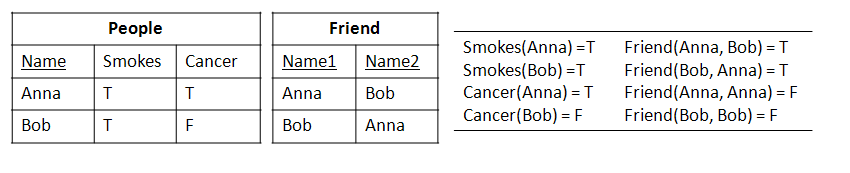
\includegraphics[width=1\textwidth]{database.png}
%}
\caption{The parents of target $\it{gender}(\U)$ in the models discovered by RDN\_Boost~(left) and RDN\_Bayes~(right). The RDN-Bayes model discovers that the gender of a user can be predicted by the gender of actors that appear in movies that the user has rated.\label{fig:dn-structure}}
\end{center}
\end{figure}



\section{Conclusion} 
\label{sec:conclusion1}
Relational dependency networks offer important advantages for modelling relational data. They can be learned quickly by first learning a Bayesian network, then performing a closed-form transformation of the Bayesian network to a dependency network. The key question is how to transform BN parameters to DN parameters. I  introduced a relational generalization of the standard propositional BN log-linear equation for the probability of a target node conditional on an assignment of values to its Markov blanket. The new log-linear equation uses a sum of expected values of BN log-conditional probabilities, with respect to a random instantiation of first-order variables. This is equivalent to using feature instantiation proportions as feature functions.  The main theorem provided a necessary and sufficient condition for when the local log-linear equations for different nodes are mutually consistent. On six benchmark datasets, learning RDNs via BNs scaled much better to large datasets than state-of-the-art functional gradient boosting methods, and provided competitive accuracy in predictions.

\chapter{Conclusion and Future Work} \label{cha:lim}
In this chapter, I summarize the system, algorithms, models and results discussed in my thesis, and I list the future directions which I am planning to work on as follows:

\paragraph{FactorBase System}
In chapter \ref{cha:system}, I  described FactorBase, a system that leverages the existing capabilities of an SQL-based RDBMS to support statistical-relational learning with respect to representational tasks and computational tasks. While FactorBase  provides good solutions for each of these system capabilities in isolation, the ease with which large complex statistical-relational objects can be integrated via SQL queries is a key feature. Because information about random variables, sufficient statistics, and models is all represented in relational database tables, a machine learning application can access and combine the information in a uniform way via SQL queries.

While my implementation has used simple SQL plus indexes, there are opportunities for optimizing RDBMS operations for the workloads required by statistical-relational structure learning. These include view materialization and the key scalability bottleneck of computing multi-relational sufficient statistics. NoSQL databases can exploit a flexible data representation for scaling to very large datasets. However, SRL requires count operations for random complex join queries, which is a challenge for less structured data representations. 

Another important goal is a single end-to-end RDBMS package for both learning and inference that integrates FactorBase with inference systems such as BayesStore, Tuffy and DeepDive \cite{Sa2016}.  This end-to-end package will be much more friendly for the consumers without much relational learning background. 
The Spark SQL module offers tighter integration between relational processing and a highly extensible optimizer tailored for the complex queries~\cite{Michael2015}. Porting FactorBase system to Spark implementation  would enhance the ability of Count Manager for processing very large-scale data sets which are beyond the capability of single RDBMS. 
Another advantage of a Spark implementation is that Spark leverages Hadoop, which is distributed file system framework for very large data sets. However, the current performance bottleneck for computing sufficient statistics is main memory not external memory.
On the other hand, incorporating the PS paradigm within Model Manager would support the distributed parameter learning for many industrial scenarios (e.g., one need to deal with very big model containing millions to billions of parameters) \cite{Li2014}.



\paragraph{Sufficient Statistics across Multiple Relationships} 
As described  in Chapter \ref{cha:multiStatistic}, the Virtual Join algorithm efficiently computes query counts which may involve any number of {\em positive and negative }relationships. These sufficient statistics support a scalable statistical analysis of associations among both relationships and attributes in a relational database. The Virtual Join algorithm scales well with the number of rows, but not with the number of columns and relationships in the database. This limitation stems from the fact that the contingency table size grows exponentially with the number of random variables in the table. 

I applied the algorithm to construct a large table for {\em all} variables in the database. I emphasize that this is not the only way to apply the algorithm. The algorithm efficiently finds cross-table statistics for any set of variables, not only for the complete set of all variables in the database. An alternative for using counting for relational model searches is to apply the Virtual Join only up to a pre-specified relatively small relationship chain length which could be determined by a learning algorithm or specified by the user. Another possibility is to use post-counting \cite{lv2012}: Rather than pre-compute a large contingency table prior to learning, compute many small contingency tables for  small subsets of variables on demand during learning. In a post-counting approach, generating a contingency table for a target set of variables is a service that can be called dynamically during the execution of a learning program. 

While I  have focused on statistical analysis, another potential application is in probabilistic first-order inference \cite{Poole2003, Hari2016}. Such inferences often require sufficient statistics with regard to counting the satisfied groundings of a first-order formula defined with respect to one or more specified individuals  (e.g.,  the number of user $\it{Jack's}$ male friends). The Virtual Join algorithm could be applied to compute sufficient statistics for specified individuals. 
In addition, the traditional ETL + single table machine learning training based model can take advantage of the sufficient statistics to gain better performance.



\paragraph{Generative Modelling with Link Uncertainty}  
I discussed two kinds of modelling approach: class-level generative modelling and instance-level discriminative learning in the context of relational data in chapter \ref{cha:lbn} and chapter \ref{cha:RDN}, respectively.  The generative modeling with Bayes net learns a model of the joint probability distribution of all input random variables. 
This type of model supports class-level queries like, ``What fraction of the grades are awarded to highly intelligent students?''
The model described in Chapter \ref{cha:lbn} captures a wider class of correlations that involve uncertainty about the link structure for complex heterogeneous network with many attributes and link types.  By capturing the relevant correlations, the model achieves better data fit on standard statistical metrics.



\paragraph {Instance Level Discriminative Learning}% 
Dependency networks are well suited for the task of discriminative learning such as classification problem to predict the label $y$ given all inputs $x$.
This type of model supports instance-level queries like, 
``What is the probability of {\em Jack} being a highly intelligent student given the grades of his registered courses?''
As introduced in chapter \ref{cha:RDN}, the hybrid approach combines the speed of learning Bayes net with the advantages of dependency network inference for relational data. Empirical experiments showed the predictive accuracy and scalability of my BN-to-DN hybrid discriminative learning algorithm. The state-of-the-art boosting approach to constructing a dependency network by learning a collection of discriminative models is very different from learning a Bayesian network. 
There are various options for hybrid approaches that combine the strengths of both, for instance:
\begin{enumerate}
\item Fast Bayesian network learning can be used to select features. Discriminative learning methods should work faster restricted to the BN Markov blanket of a target node. 
\item The Bayesian network can provide an initial dependency network structure. Gradient boosting can then be used to fine-tune local distribution models.
\end{enumerate}


\paragraph{Integrated Statistical Analysis for Complex Heterogeneous Data}
Many real world datasets are relational and most real world applications are characterized by the presence of uncertainty and complex relational structures. In the thesis, I focus on statistical modelling of the interactions between different descriptive attributes and the link itself for complex heterogeneous and richly interconnected data.
The SQL-based FactorBase system provides integrated statistical analysis out-of-the-box for challenging applications on two folds: the class-level generative modelling with Bayes net and the instance-level discriminative learning with relational dependency networks.  All statistical objects are stored as first-class citizens as well as  raw data; one can access and combine the information in a uniform way via SQL queries. The Virtual Join algorithm solves the scalability bottleneck for using cross-table sufficient statistics in relational model searching. The model captures a wider class of correlations that involve uncertainty about the link structure.
 


\backmatter%
	\addtoToC{Bibliography}
	\bibliographystyle{plain}
	\bibliography{master} 

\let\svaddcontentsline\addcontentsline
\renewcommand\addcontentsline[3]{%
  \ifthenelse{\equal{#1}{lof}}{}%
  {\ifthenelse{\equal{#1}{lot}}{}{\svaddcontentsline{#1}{#2}{#3}}}}

\begin{appendices} % optional
\chapter{ Proof of Consistency Characterization}

This appendix presents a proof of Theorem~\ref{th:consistent-dn}. The theorem says that a dependency network derived from a template Bayesian network is consistent if and only if the Bayesian network is edge-consistent. I  begin by showing that Bayesian network edge-consistency is sufficient for dependency network consistency. This is the easy direction. That edge-consistency is also necessary requires several intermediate results.

\section{Edge-Consistency is Sufficient for Consistency}

Edge consistency entails that each grounding of a node determines a unique grounding of both its parents and its children in the Bayesian network. Thus the ground dependency network is composed of disjoint dependency networks, one for each grounding. Each of the ground disjoint dependency networks is consistent, so a joint distribution over all can be defined as the product of the joint probabilities of each ground dependency network. The formal statement and proof is as follows.

\begin{proposition}
If a template Bayesian network is edge-consistent, then the derived dependency network is consistent.
\end{proposition}

\begin{proof} Heckermann {\em et al.}~\cite{Heckerman2000} showed that a dependency network is consistent if and only if there is a Markov network with the same graphical structure that agrees with the local conditional distributions. I  argue that given edge-consistency, there is such a Markov network for the derived dependency network. This Markov network  is obtained by moralizing and then grounding the Bayesian network~\cite{Domingos2009}. Given edge-consistency, for each ground target node, each family of the ground target node has a unique grounding. Thus the relevant family counts are all either 1 or 0 (0 if the family configuration is irrelevant). The Markov network is now defined as follows: Each grounding of a family in the template Bayesian network is a clique. For an assignment of values $\FG{\UT} = \UV,\FG{\Pa{\UT}} = \Prange{\UT}$ to a ground family, the clique potential is 1 if the assignment is irrelevant, and $\cprob{\UT = \UV}{\Pa{\UT} = \Prange{\UT}}$ otherwise. It is easy to see that the conditional distributions induced by this Markov network agree with those defined by Equation~\ref{def:log-diff-freq-eq}, given edge-consistency.
\end{proof}

\section{Edge-Consistency is Necessary for Consistency} 
This direction requires a mild condition on the structure of the Bayesian network: it must not contain a redundant edge \cite{Pearl1988}. An edge $\TT_{1}\rightarrow \TT_{2}$ is redundant if for every value of the parents of $\TT_{2}$ excluding $\TT_{1}$, every value of $\TT_{1}$ is conditionally independent of every value of $\TT_{2}$. Less formally, given the other parents, the node $\TT_{1}$ adds no probabilistic information about the child node $\TT_{2}$. Throughout the remainder of the proof, I  assume that the template Bayesian network contains no redundant edges.
The proof is based on establishing the following theorem. 

\begin{theorem}\label{theorem:inconsistency-condition}
Assume that a template BN contains at least one edge $e_1$ such that the parent and child do not contain the same set of population variables. Then there exists an edge $e_2$ (which may be the same as or distinct from $e_1$) from parent $\TT_{1}$ to child $\TT_{2}$, ground nodes $\FG{\TT_{1}}$ and $\FG{\TT_{2}}$,  and a query conjunction $\QC$ such that: the ground nodes $\FG{\TT_{1}}$ and $\FG{\TT_{2}}$ have mutually inconsistent conditional distributions $\cprob{\FG{\TT_{1}}}{\QC}$ and $\cprob{\FG{\TT_{2}}}{\QC}$ as defined by Equation~\ref{def:log-diff-freq-eq}.
\end{theorem}

The query conjunction $\QC$ here denotes a complete specification of all values for all ground nodes except for $\FG{\TT_{1}}$ and $\FG{\TT_{2}}$. Theorem~\ref{theorem:inconsistency-condition} entails the necessity direction of Theorem~\ref{th:consistent-dn} by the following argument. Suppose that there is a joint distribution $p$ that agrees with the conditional distributions of the derived dependency network. Then for every query conjunction $\QC$, and for every assignment of values $\TV_{1}$ resp. $\TV_{2}$ to the ground nodes, I   have that $p(\FG{\TT_{1}}=\TV_{1}|\FG{\TT_{2}}=\TV_{2},\QC)$ and $p(\FG{\TT_{2}}=\TV_{2}|\FG{\TT_{1}}=\TV_{1},\QC)$ agree with the log-linear equation~\ref{def:log-diff-freq-eq}. Therefore, the conditional distributions $p(\FG{\TT_{1}}|\FG{\TT_{2}},\QC)$ and $p(\FG{\TT_{2}}|\FG{\TT_{1}},\QC)$ must be mutually consistent. 
Theorem~\ref{theorem:inconsistency-condition} asserts that for every (non-redundant) edge-inconsistent template BN, I  can find a query conjunction and two ground nodes such that the conditional distributions of the ground nodes given the query conjunction are not mutually consistent. Therefore there is no joint distribution that is consistent with all the conditional distributions defined by the log-linear equations, which establishes the necessity direction of the main theorem~\ref{th:consistent-dn}. 

\subsection{Properties of the template BN and the input query $\QC$}
I  begin by establishing some properties of the template BN and the query conjunction that are needed in the remainder of the proof.
%


%\subsection{Properties of the template BN and the input query $\QC$} 
The inconsistency of the BN networks arises when a parent and a child ground node have different relevant family counts. The next lemma shows that this is possible exactly when the template BN is properly relational, meaning it relates parents and children from different populations.

\begin{lemma} \label{lemma:grounding} The following conditions are equivalent for a template edge $\TT_{1} \rightarrow \TT_{2}$.
\begin{enumerate}
\item The parent and child do not contain the same population variables.
\item It is possible to find a grounding $\grounding$ for both parent and child, and an assignment $\QC$ to all other nodes, such that the relevant family count for the $\TT_{2}$ family differs for $\FG{\TT_{1}} = \grounding \TT_{1}$ 
and $\FG{\TT_{2}} = \grounding \TT_{2}$.
\end{enumerate}
\end{lemma}

\begin{proof}
If the parent and child contain the same population variables, then there is a 1-1 correspondence between groundings of the child and groundings of the parents. Hence the count of relevant family groundings is the same for each, no matter how parents and child are instantiated. If the parent and child do not contain the same population variables, suppose without loss of generality that the child contains a population variable $\A$ not contained in the parent. Choose a common grounding $\grounding$ for the parents and child node. For the ground child node, $\grounding \TT_{2}$, let $\grounding$ be the only family grounding that is relevant, so the relevant count is 1. For the  ground parent node, there is at least one other grounding of the child node $\TT_{2}'$ different from $\grounding \TT_{2}$ since $\TT_{2}$ contains another population variables. Thus it is possible to add another relevant family grounding for $\grounding \TT_{1}$, which means that the relevant count is at least 2. 
\end{proof}
The proof proceeds most simply if I  focus on template edges that relate different populations and no common children.

\begin{definition} \label{def:suitable}
An template edge $\TT_{1} \rightarrow \TT_{2}$ is \defterm{suitable} if
\begin{enumerate}
\item The parent and child do not contain the same population variables.
\item The parent and child have no common edge.
\end{enumerate}
\end{definition}
The next lemma shows that focusing on suitable edges incurs no loss of generality.

\begin{lemma} \label{lemma:suitable}
Suppose that a template BN contains an edge such that the parent and child do not contain the same population variables. Then the template BN contains a suitable edge. 
\end{lemma}

\begin{proof}
Suppose that there is an edge satisfying the population variable condition. Suppose that the parent and child share a common child. Since the edge satisfies the condition, the set of population variables in the common child differs from at least one of  $\TT_{1}, \TT_{2}$. Therefore there is another edge from one of  $\TT_{1} \rightarrow \TT_{2}$ as parent to a new child that satisfies the population variable condition. If this edge is not suitable, there must be another shared child. Repeating this argument, I  eventually arrive at an edge satisfying the population variable condition  where the child node is a sink node without children. This edge is suitable.
\end{proof}

Consider a suitable template edge $\TT_{1} \rightarrow \TT_{2}$ that produces a bidirected ground edge $\FG{\TT_{1}} \leftrightarrow \FG{\TT_{2}}$. For simplicity I  assume that $\TT_{1}$ and $\TT_{2}$ are binary variables with domain $\{\true,\false\}$. (This incurs no loss of generality as I  can choose a database $\QC$ in which only two values occur.) Let $\Pa{\TT_{2}}$ be the parents of $\TT_{2}$ other than $\TT_{1}$. Since the template edge is not redundant \cite{Pearl1988}, there is a parent value setting $\Pa{\TT_{2}} = \parents$ such that $\TT_{1}$ and $\TT_{2}$ are conditionally dependent given $\Pa{\TT_{2}} = \parents$. This implies that the conditional distribution of $\TT_{1}$ is different for each of the two possible values of $\TT_{2}$:
% In terms of the template Bayesian network parameters, this implies that
\begin{equation} \label{eq:dependence}
\frac{\cprob{\TT_{2} = \false}{\TT_{1} = \false,\parents}}{\cprob{\TT_{2} = \true}{\TT_{1} = \false,\parents}} \neq \frac{\cprob{\TT_{2} = \false}{\TT_{1} = \true,\parents}}{\cprob{\TT_{2} = \true}{\TT_{1} = \true,\parents}}.
\end{equation}
Let $\QC$ denote an assignment of values to all ground nodes other than the target nodes $\FG{\TT_{1}}$ and $ \FG{\TT_{2}}$. I  assume that the input query $\QC$ assigns different relevant family counts $N_{1}$ to $\FG{\TT_{1}}$ and $N_{2}$ to $\FG{\TT_{2}}$. This is possible according to Lemma~\ref{lemma:grounding}. 
\subsubsection{Lowd's Equation and Relevant Family Counts}
The log-linear equation~\ref{def:log-diff-freq-eq}, specifies the conditional distribution of each target node given $\QC$ and a value for the other target node. I  keep the assignment $\QC$ fixed throughout, so for more compact notation, I  abbreviate the conditional distributions as
$$\joint(\FG{{\TT_{1}}} = \TV_{1}| \FG{{\TT_{2}}} = \TV_{2}) \equiv P(\FG{{\TT_{1}}} = \TV_{1}|\FG{{\TT_{2}}} = \TV_{2},\QC)$$ 
and similarly for $P(\FG{{\TT_{1}}} = \TV_{1}|\FG{{\TT_{2}}} = \TV_{2},\QC)$.

On the assumption that the dependency network is consistent, there is a joint distribution over the target nodes conditional on the assignment that agrees with the conditional distribution:
$$\frac{\joint(\FG{{\TT_{1}}} = \TV_{1}, \FG{{\TT_{2}}} = \TV_{2})}{\joint(\FG{{\TT_{2}}} = \TV_{2})}= \joint(\FG{{\TT_{1}}} = \TV_{1}| \FG{{\TT_{2}})}$$
and also with the conditional $\joint(\FG{{\TT_{2}}} = \TV_{2}| \FG{{\TT_{1}}}=\TV_{1}).$

Lowd \cite{Lowd2012} pointed out that this joint distribution satisfies the equations
\begin{equation}  \frac{\joint(\false,\false)}{\joint(\true,\false)} \cdot \frac{\joint(\true,\false)}{\joint(\true,\true)}= \frac{\joint(\false,\false)}{\joint(\true,\true)} = \frac{\joint(\false,\false)}{\joint(\false,\true)} \cdot \frac{\joint(\false,\true)}{\joint(\true,\true)} \label{eq:lowd-joint}
\end{equation}

Since the ratio of joint probabilities is the same as the ratio of conditional probabilities for the same conditioning event, consistency entails the following constraint on conditional probabilities via Equation~\eqref{eq:lowd-joint}:

{\small
\begin{equation}
\frac{\joint(\FG{{\TT_{2}}}=\false|\FG{{\TT_{1}}}=\false)}{\joint(\FG{{\TT_{2}}} = \true| \FG{{\TT_{1}}}=\false)} \cdot \frac{\joint(\FG{{\TT_{1}}}=\false|\FG{{\TT}_{2}}=\true)}{\joint(\FG{{\TT_{1}}} = \true| \FG{{\TT_{2}}}=\true)} =\frac{\joint(\FG{{\TT_{1}}}=\false|\FG{{\TT_{2}}}=\false)}{\joint(\FG{{\TT_{1}}} = \true| \FG{{\TT_{2}}}=\false)} \cdot \frac{\joint(\FG{{\TT_{2}}}=\false|\FG{{\TT_{1}}}=\true)}{\joint(\FG{{\TT_{2}}} = \true| \FG{{\TT_{1}}}=\true)} \label{eq:lowd-conditional}
\end{equation}
}I  refer to Equation~\ref{eq:lowd-conditional} as {\em Lowd's equation}. 
The idea of the proof is to show that Lowd's equations are satisfied only if the relevant family counts for the target nodes are the same. According to the log-linear equation, each conditional probability is proportional to a product of BN parameters. The first step is to show that in Lowd's equation, all BN parameter terms cancel out except for those that are derived from the family that comprises $\FG{\TT_{1}}$ and their $\FG{\TT_{2}}$ and their common grounding. 

\begin{lemma} \label{lemma:decompose-cond} The conditional probabilities for the target nodes can be written as follows:
\begin{equation}
\Gprob{\FG{{\TT_{2}}} = \TV_{2}} {\FG{\TT_{1}} = \TV_{1},\QC} \propto \cprob{\TT_{2} = \TV_{2}}{\TT_{1} = \TV_{1},\parents}^{(N/N_{2}+M_{\TT_2=\TV_{2}}/N_{2})} \cdot \pi_{\TT_2=\TV_{2}} \label{eq:decompose-t2}
\end{equation}
where $M_{\TT_2=\TV_{2}}$ and $\pi_{\TT_2=\TV_{2}}$ depend only on $\TV_{2}$ and not on $\TV_{1}$ and
\begin{equation}
\Gprob{\FG{{\TT_{1}}} = \TV_{1}} {\FG{\TT_{2}} = \TV_{2},\QC} \propto \cprob{\TT_{2} = \TV_{2}}{\TT_{1} = \TV_{1},\parents}^{(N/N_{1}+M_{\TT_1=\TV_{1}}/N_{1})} \cdot \pi_{\TT_1=\TV_{1}} \label{eq:decompose-t1}
\end{equation} 
where $M_{\TT_1=\TV_{1}}$ and $\pi_{\TT_1=\TV_{1}}$ depend only on $\TV_{1}$ and not on $\TV_{2}$.
\end{lemma}

\paragraph{Proof Outline.} This is based on analysing the different types of families that appear in the log-linear equation and their groundings. I  omit this straightforward analysis to simplify the proof; the details are available from \cite{Schulte2014a}.

%\marginpar{add full proof to archive}


\begin{lemma} \label{lemma:family-agree}
Suppose that conditions~\eqref{eq:decompose-t2} and~\eqref{eq:decompose-t1} of Lemma~\ref{lemma:decompose-cond} hold. Then Lowd's Equation~\eqref{eq:lowd-conditional} holds if and only if $N_{1} = N_{2}$. 
\end{lemma}

\begin{proof}
Observe that in Equation~\eqref{eq:lowd-conditional}, each term on the left has a corresponding term with the same value for the target node assignment and the opposing conditioning assignment. For instance, the term $\joint(\FG{{\TT_{2}}}=\false|\FG{{\TT_{1}}}=\false)$ on the left is matched with the term $\joint(\FG{{\TT_{2}}}=\false|\FG{{\TT_{1}}}=\true)$ on the right. This means that the products in the log-linear expression are the same on both sides of the equation except for those factors that depend on {\em both} $\TV_{1}$ and $\TV_{2}$. Continuing the example, the factors $$\cprob{\TT_{2} = \false}{\TT_{1} = \false,\parents}^{(M_{\false}/N_{2})} \cdot \pi_{\TT_2=\TV_{2}}$$ on the left equal the factors $$\cprob{\TT_{2} = \false}{\TT_{1} = \true,\parents}^{(M_{\TT_1=\TV_{1}}/N_{2})}\cdot \pi_{\TT_2=\TV_{2}}$$ on the right side of the equation. They therefore cancel out, leaving only the term $$\cprob{\TT_{2} = \false}{\TT_{1} = \false,\parents}^{N/N_{2}}$$ on the left and the term $$\cprob{\TT_{2} = \false}{\TT_{1} = \false,\parents}^{N/N_{2}}$$ on the right. Lowd's equation can therefore be reduced to an equivalent constraint with only such BN parameter terms. For further compactness I  abbreviate such terms as follows
%
$$\cprob{\TV_{2}}{\TV_{1}} \equiv \cprob{\TT_{2} = \TV_{2}}{\TT_{1} = \TV_{1},\parents}.$$ With this abbreviation, the conditions of Lemma~\ref{lemma:decompose-cond} entail that Lowd's equation~\ref{eq:lowd-conditional} reduces to the equivalent expressions.
%
\begin{eqnarray}
\frac{\cprob{\false}{\false}^{N/N_{2}}}{\cprob{\true}{\false}^{N/N_{2}} }  \cdot \frac{\cprob{\true}{\false}^{N/N_{1}} }{\cprob{\true}{\true}^{N/N_{1}} }  & = & \frac{\cprob{\false}{\false}^{N/N_{1}} }{\cprob{\false}{\true}^{N/N_{1}} }  \cdot \frac{\cprob{\false}{\true}^{N/N_{2}} }{\cprob{\true}{\true}^{N/N_{2}} } \\
(\frac{\cprob{\false}{\false}}{\cprob{\true}{\false} })^{\left(N/N_{2}-N/N_{1}\right)}   & = &  (\frac{\cprob{\false}{\true} }{\cprob{\true}{\true}})^{\left(N/N_{2}-N/N_{1}\right)} \label{eq:transform-ratio}
\end{eqnarray}
By the nonredundancy  assumption~\eqref{eq:dependence} on the BN parameters, I  have
%
$$\frac{\cprob{\false}{\false}}{\cprob{\true}{\false} }   \neq  \frac{\cprob{\false}{\true} }{\cprob{\true}{\true}}$$

so Equation~\ref{eq:transform-ratio} implies that 
%
$$N_{1} = N_{2}, $$ which establishes the lemma. 
\end{proof}

Theorem~\ref{theorem:inconsistency-condition} now follows as follows: Lemma~\ref{lemma:grounding} entails that if the dependency network is consistent, the log-linear equations satisfy Lowd's equation with the bidirected ground edge $\FG{\TT_{1}} \leftrightarrow \FG{\TT_{2}}$ and the query conjunction $\QC$ that satisfies the BN non-redundancy condition. Lemmas~\ref{eq:lowd-conditional} and~\ref{lemma:suitable} show that if the template BN is relational, it must contain a suitable edge $\TT_{1} \rightarrow \TT_{2}$. Lemma~\ref{lemma:family-agree} 
 together with Lowd's equation entails that the relevant counts for $\FG{\TT_{1}}$ and $\FG{\TT_{2}}$ must then be the same. But the query conjunction $\QC$ was chosen so that the relevant counts are different. This contradiction shows that Lowd's equation is unsatisfiable, and therefore no joint distribution exists that is consistent with the BN conditional distributions specified by the log-linear Equation~\ref{def:log-diff-freq-eq}. Since Theorem~\ref{theorem:inconsistency-condition} entails Theorem~\ref{th:consistent-dn}, the proof is complete.

\end{appendices}


\begin{appendices} % optional
\chapter{ }
\section {SQL Queries for Achema Analyzer}

\begin{alltt}

DROP SCHEMA IF EXISTS @database@_AchemaAnalyzer; 
CREATE SCHEMA  @database@_AchemaAnalyzer;

CREATE SCHEMA  if not exists @database@_BN;
CREATE SCHEMA  if not exists @database@_CT;

USE @database@_AchemaAnalyzer;
SET storage_engine=INNODB;

CREATE TABLE Schema_Key_Info AS SELECT TABLE_NAME, COLUMN_NAME,
REFERENCED_TABLE_NAME, REFERENCED_COLUMN_NAME, CONSTRAINT_NAME FROM
INFORMATION_SCHEMA.KEY_COLUMN_USAGE WHERE (KEY_COLUMN_USAGE.TABLE_SCHEMA =
'@database@') ORDER BY TABLE_NAME;

CREATE TABLE Schema_Position_Info AS SELECT COLUMNS.TABLE_NAME,
COLUMNS.COLUMN_NAME,
COLUMNS.ORDINAL_POSITION FROM
INFORMATION_SCHEMA.COLUMNS,
INFORMATION_SCHEMA.TABLES
WHERE
(COLUMNS.TABLE_SCHEMA = '@database@'
    AND TABLES.TABLE_SCHEMA = '@database@'
    AND TABLES.TABLE_NAME = COLUMNS.TABLE_NAME
    AND TABLES.TABLE_TYPE = 'BASE TABLE')
ORDER BY TABLE_NAME;

CREATE TABLE NoPKeys AS SELECT TABLE_NAME FROM
Schema_Key_Info
WHERE
TABLE_NAME NOT IN (SELECT 
        TABLE_NAME
    FROM
        Schema_Key_Info
    WHERE
        CONSTRAINT_NAME LIKE 'PRIMARY');

CREATE table NumEntityColumns AS
SELECT 
    TABLE_NAME, COUNT(DISTINCT COLUMN_NAME) num
FROM
    Schema_Key_Info
WHERE
    CONSTRAINT_NAME LIKE 'PRIMARY'
        OR REFERENCED_COLUMN_NAME IS NOT NULL
GROUP BY TABLE_NAME;

CREATE TABLE TernaryRelations as SELECT TABLE_NAME FROM
NumEntityColumns
WHERE
num > 2;

CREATE TABLE KeyColumns AS SELECT * FROM
(Schema_Key_Info
NATURAL JOIN Schema_Position_Info)
WHERE
TABLE_NAME NOT IN (SELECT 
        TABLE_NAME
    FROM
        NoPKeys)
    AND TABLE_NAME NOT IN (SELECT 
        TABLE_NAME
    FROM
        TernaryRelations);

CREATE TABLE AttributeColumns AS SELECT TABLE_NAME, COLUMN_NAME FROM
Schema_Position_Info
WHERE
(TABLE_NAME , COLUMN_NAME) NOT IN (SELECT 
        TABLE_NAME, COLUMN_NAME
    FROM
        KeyColumns)
    and TABLE_NAME NOT IN (SELECT 
        TABLE_NAME
    FROM
        NoPKeys)
    and TABLE_NAME NOT IN (SELECT 
        TABLE_NAME
    FROM
        TernaryRelations);

ALTER TABLE AttributeColumns ADD PRIMARY KEY (TABLE_NAME,COLUMN_NAME);

CREATE TABLE InputColumns AS SELECT * FROM
KeyColumns
WHERE
CONSTRAINT_NAME = 'PRIMARY'
ORDER BY TABLE_NAME;

CREATE TABLE ForeignKeyColumns AS SELECT * FROM
KeyColumns
WHERE
REFERENCED_COLUMN_NAME IS NOT NULL
ORDER BY TABLE_NAME;

ALTER TABLE ForeignKeyColumns
 ADD PRIMARY KEY (TABLE_NAME,COLUMN_NAME,REFERENCED_TABLE_NAME);

CREATE TABLE EntityTables AS SELECT distinct TABLE_NAME, COLUMN_NAME FROM
KeyColumns T
WHERE
1 = (SELECT 
        COUNT(COLUMN_NAME)
    FROM
        KeyColumns T2
    WHERE
        T.TABLE_NAME = T2.TABLE_NAME
            AND CONSTRAINT_NAME = 'PRIMARY');

ALTER TABLE EntityTables ADD PRIMARY KEY (TABLE_NAME,COLUMN_NAME);

CREATE TABLE SelfRelationships AS
 SELECT DISTINCT RTables1.TABLE_NAME AS TABLE_NAME,
RTables1.REFERENCED_TABLE_NAME AS REFERENCED_TABLE_NAME,
RTables1.REFERENCED_COLUMN_NAME AS REFERENCED_COLUMN_NAME FROM
KeyColumns AS RTables1,
KeyColumns AS RTables2
WHERE
(RTables1.TABLE_NAME = RTables2.TABLE_NAME)
    AND (RTables1.REFERENCED_TABLE_NAME = RTables2.REFERENCED_TABLE_NAME)
    AND (RTables1.REFERENCED_COLUMN_NAME = RTables2.REFERENCED_COLUMN_NAME)
    AND (RTables1.ORDINAL_POSITION < RTables2.ORDINAL_POSITION);

ALTER TABLE SelfRelationships ADD PRIMARY KEY (TABLE_NAME);

CREATE TABLE Many_OneRelationships AS SELECT KeyColumns1.TABLE_NAME FROM
KeyColumns AS KeyColumns1,
KeyColumns AS KeyColumns2
WHERE
(KeyColumns1.TABLE_NAME , KeyColumns1.COLUMN_NAME) IN (SELECT 
        TABLE_NAME, COLUMN_NAME
    FROM
        InputColumns)
    AND (KeyColumns2.TABLE_NAME , KeyColumns2.COLUMN_NAME) IN (SELECT 
        TABLE_NAME, COLUMN_NAME
    FROM
        ForeignKeyColumns)
    AND (KeyColumns2.TABLE_NAME , KeyColumns2.COLUMN_NAME) NOT IN (SELECT 
        TABLE_NAME, COLUMN_NAME
    FROM
        InputColumns);

CREATE TABLE PVariables AS SELECT CONCAT(EntityTables.TABLE_NAME, '0') AS Pvid,
EntityTables.TABLE_NAME,
0 AS index_number FROM
EntityTables 
UNION 
SELECT 
CONCAT(EntityTables.TABLE_NAME, '1') AS Pvid,
EntityTables.TABLE_NAME,
1 AS index_number
FROM
EntityTables,
SelfRelationships
WHERE
EntityTables.TABLE_NAME = SelfRelationships.REFERENCED_TABLE_NAME
    AND EntityTables.COLUMN_NAME = SelfRelationships.REFERENCED_COLUMN_NAME ;

ALTER TABLE PVariables ADD PRIMARY KEY (Pvid);

CREATE TABLE RelationTables AS SELECT DISTINCT ForeignKeyColumns.TABLE_NAME,
ForeignKeyColumns.TABLE_NAME IN (SELECT 
        TABLE_NAME
    FROM
        SelfRelationships) AS SelfRelationship,
ForeignKeyColumns.TABLE_NAME IN (SELECT 
        TABLE_NAME
    FROM
        Many_OneRelationships) AS Many_OneRelationship FROM
ForeignKeyColumns;

ALTER TABLE RelationTables ADD PRIMARY KEY (TABLE_NAME);

CREATE TABLE 1Variables AS
 SELECT CONCAT('`', COLUMN_NAME, '(', Pvid, ')', '`') AS 1VarID,
COLUMN_NAME,
Pvid,
index_number = 0 AS main FROM
PVariables
    NATURAL JOIN
AttributeColumns;

ALTER TABLE 1Variables ADD PRIMARY KEY (1VarID);
ALTER TABLE 1Variables ADD UNIQUE(Pvid,COLUMN_NAME);

CREATE TABLE ForeignKeys_pvars AS SELECT ForeignKeyColumns.TABLE_NAME,
ForeignKeyColumns.REFERENCED_TABLE_NAME,
ForeignKeyColumns.COLUMN_NAME,
Pvid,
index_number,
ORDINAL_POSITION AS ARGUMENT_POSITION FROM
ForeignKeyColumns,
PVariables
WHERE
PVariables.TABLE_NAME = REFERENCED_TABLE_NAME;

ALTER TABLE ForeignKeys_pvars ADD PRIMARY KEY (TABLE_NAME,Pvid,ARGUMENT_POSITION);

CREATE table Relationship_MM_NotSelf AS
SELECT 
    CONCAT('`',
            ForeignKeys_pvars1.TABLE_NAME,
            '(',
            ForeignKeys_pvars1.Pvid,
            ',',
            ForeignKeys_pvars2.Pvid,
            ')',
            '`') AS orig_RVarID,
    ForeignKeys_pvars1.TABLE_NAME,
    ForeignKeys_pvars1.Pvid AS Pvid1,
    ForeignKeys_pvars2.Pvid AS Pvid2,
    ForeignKeys_pvars1.COLUMN_NAME AS COLUMN_NAME1,
    ForeignKeys_pvars2.COLUMN_NAME AS COLUMN_NAME2,
    (ForeignKeys_pvars1.index_number = 0
        AND ForeignKeys_pvars2.index_number = 0) AS main
FROM
    ForeignKeys_pvars AS ForeignKeys_pvars1,
    ForeignKeys_pvars AS ForeignKeys_pvars2,
    RelationTables
WHERE
    ForeignKeys_pvars1.TABLE_NAME = ForeignKeys_pvars2.TABLE_NAME
        AND RelationTables.TABLE_NAME = ForeignKeys_pvars1.TABLE_NAME
        AND ForeignKeys_pvars1.ARGUMENT_POSITION 
        		    < ForeignKeys_pvars2.ARGUMENT_POSITION
        AND RelationTables.SelfRelationship = 0
        AND RelationTables.Many_OneRelationship = 0;

CREATE table Relationship_MM_Self AS
SELECT 
    CONCAT('`',
            ForeignKeys_pvars1.TABLE_NAME,
            '(',
            ForeignKeys_pvars1.Pvid,
            ',',
            ForeignKeys_pvars2.Pvid,
            ')',
            '`') AS orig_RVarID,
    ForeignKeys_pvars1.TABLE_NAME,
    ForeignKeys_pvars1.Pvid AS Pvid1,
    ForeignKeys_pvars2.Pvid AS Pvid2,
    ForeignKeys_pvars1.COLUMN_NAME AS COLUMN_NAME1,
    ForeignKeys_pvars2.COLUMN_NAME AS COLUMN_NAME2,
    (ForeignKeys_pvars1.index_number = 0
        AND ForeignKeys_pvars2.index_number = 1) AS main
FROM
    ForeignKeys_pvars AS ForeignKeys_pvars1,
    ForeignKeys_pvars AS ForeignKeys_pvars2,
    RelationTables
WHERE
    ForeignKeys_pvars1.TABLE_NAME = ForeignKeys_pvars2.TABLE_NAME
        AND RelationTables.TABLE_NAME = ForeignKeys_pvars1.TABLE_NAME
        AND ForeignKeys_pvars1.ARGUMENT_POSITION
        			 < ForeignKeys_pvars2.ARGUMENT_POSITION
        AND ForeignKeys_pvars1.index_number < ForeignKeys_pvars2.index_number
        AND RelationTables.SelfRelationship = 1
        AND RelationTables.Many_OneRelationship = 0;

CREATE table Relationship_MO_NotSelf AS
SELECT 
    CONCAT('`',
            ForeignKeys_pvars.REFERENCED_TABLE_NAME,
            '(',
            PVariables.Pvid,
            ')=',
            ForeignKeys_pvars.Pvid,
            '`') AS orig_RVarID,
    ForeignKeys_pvars.TABLE_NAME,
    PVariables.Pvid AS Pvid1,
    ForeignKeys_pvars.Pvid AS Pvid2,
    KeyColumns.COLUMN_NAME AS COLUMN_NAME1,
    ForeignKeys_pvars.COLUMN_NAME AS COLUMN_NAME2,
    (PVariables.index_number = 0
        AND ForeignKeys_pvars.index_number = 0) AS main
FROM
    ForeignKeys_pvars,
    RelationTables,
    KeyColumns,
    PVariables
WHERE
    RelationTables.TABLE_NAME = ForeignKeys_pvars.TABLE_NAME
        AND RelationTables.TABLE_NAME = PVariables.TABLE_NAME
        AND RelationTables.TABLE_NAME = KeyColumns.TABLE_NAME
        AND RelationTables.SelfRelationship = 0
        AND RelationTables.Many_OneRelationship = 1;

CREATE table Relationship_MO_Self AS
SELECT 
    CONCAT('`',
            ForeignKeys_pvars.REFERENCED_TABLE_NAME,
            '(',
            PVariables.Pvid,
            ')=',
            ForeignKeys_pvars.Pvid,
            '`') AS orig_RVarID,
    ForeignKeys_pvars.TABLE_NAME,
    PVariables.Pvid AS Pvid1,
    ForeignKeys_pvars.Pvid AS Pvid2,
    KeyColumns.COLUMN_NAME AS COLUMN_NAME1,
    ForeignKeys_pvars.COLUMN_NAME AS COLUMN_NAME2,
    (PVariables.index_number = 0
        AND ForeignKeys_pvars.index_number = 1) AS main
FROM
    ForeignKeys_pvars,
    RelationTables,
    KeyColumns,
    PVariables
WHERE
    RelationTables.TABLE_NAME = ForeignKeys_pvars.TABLE_NAME
        AND RelationTables.TABLE_NAME = PVariables.TABLE_NAME
        AND RelationTables.TABLE_NAME = KeyColumns.TABLE_NAME
        AND PVariables.index_number < ForeignKeys_pvars.index_number
        AND RelationTables.SelfRelationship = 1
        AND RelationTables.Many_OneRelationship = 1;

CREATE TABLE Relationship AS SELECT * FROM  
Relationship_MM_NotSelf    
UNION SELECT            
*                   
FROM
Relationship_MM_Self 
UNION SELECT 
*
FROM
Relationship_MO_NotSelf 
UNION SELECT 
*
FROM
Relationship_MO_Self;

ALTER TABLE Relationship ADD PRIMARY KEY (orig_RVarID);
ALTER TABLE `Relationship` ADD COLUMN `RVarID` 
	VARCHAR(10) NULL , ADD UNIQUE INDEX `RVarID_UNIQUE` (`RVarID` ASC) ; 


CREATE TABLE 2Variables AS SELECT CONCAT('`',
        COLUMN_NAME,
        '(',
        Pvid1,
        ',',
        Pvid2,
        ')',
        '`') AS 2VarID,
COLUMN_NAME,
Pvid1,
Pvid2,
TABLE_NAME,
main FROM
Relationship
    NATURAL JOIN
AttributeColumns;

ALTER TABLE 2Variables ADD PRIMARY KEY (2VarID);</p>\end{alltt}

%\section{Final Thoughts on Good Layout}
%Please use readable font sizes in the figures and graphs. Avoid tempering with the correct border values, and the spacing (and format) of both text and captions of the PVLDB format (e.g. captions are bold).
%
%At the end, please check for an overall pleasant layout, e.g. by ensuring a readable and logical positioning of any floating figures and tables. Please also check for any line overflows, which are only allowed in extraordinary circumstances (such as wide formulas or URLs where a line wrap would be counterintuitive).
%
%Use the \texttt{balance} package together with a \texttt{\char'134 balance} command at the end of your document to ensure that the last page has balanced (i.e. same length) columns.



\section {Tables  Dependency in the Random Variable Database $\RVD$}
\begin{figure}[H]
\begin{center}
\resizebox{1\textwidth}{!}{
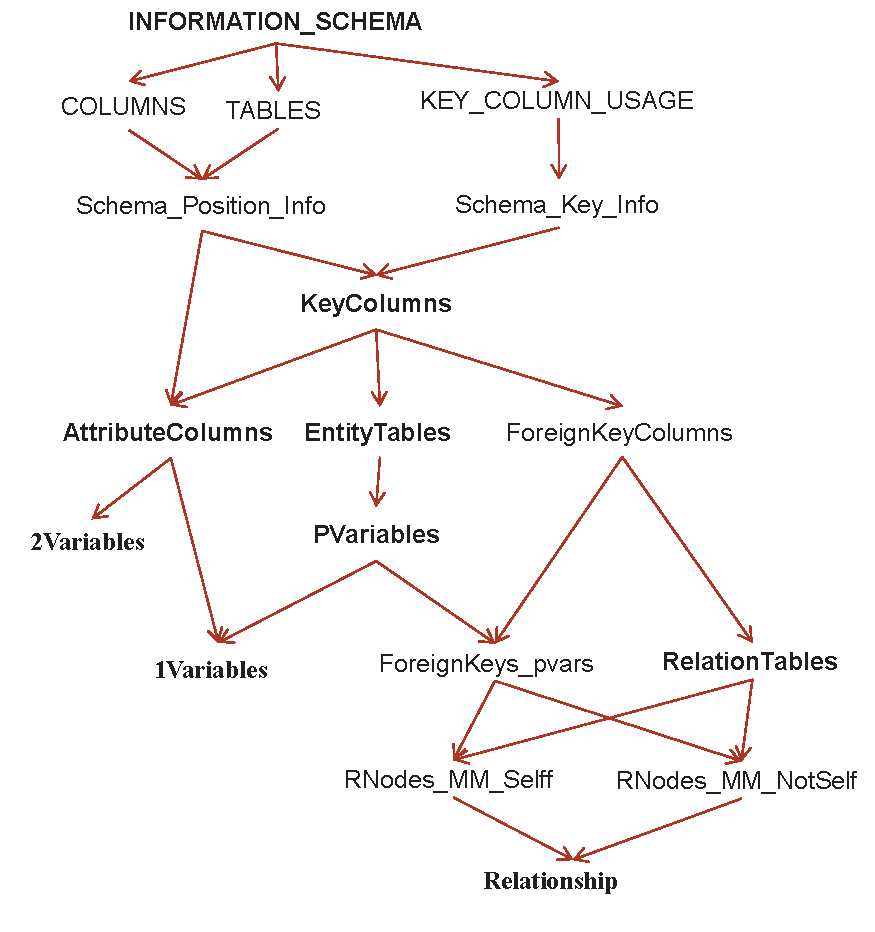
\includegraphics[width=1\textwidth]{rv_db.pdf} %move to the appendix
%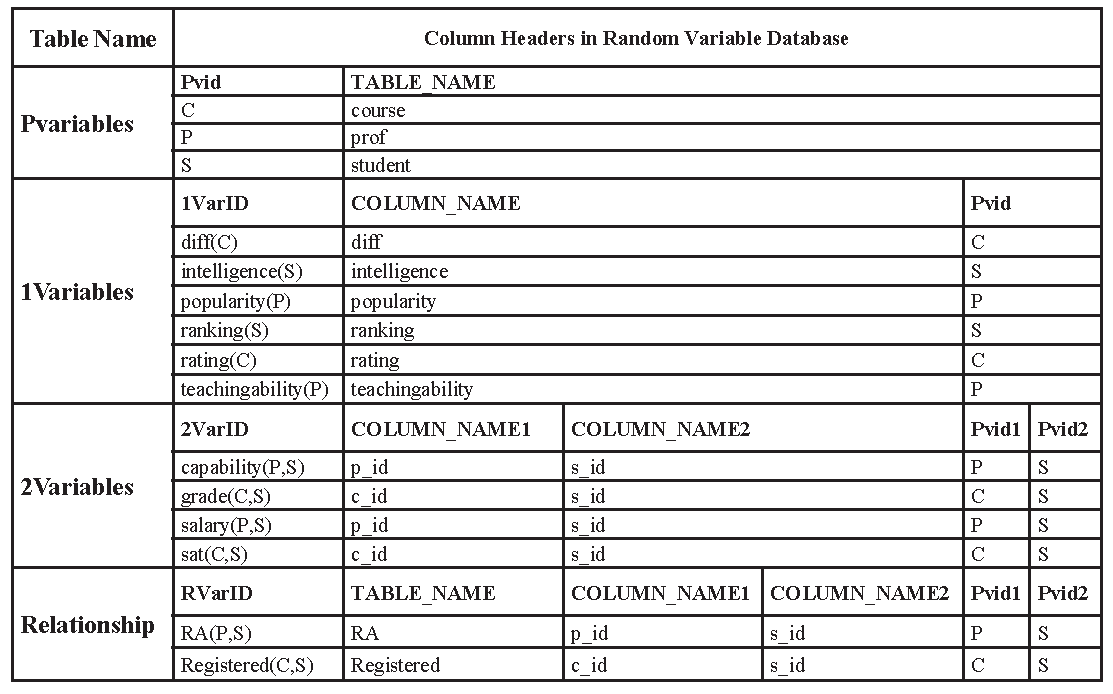
\includegraphics[width=0.5\textwidth]{rv_db_tables.pdf}
}
\caption{Tables  Dependency in the Random Variable Database $\RVD$.
\label{fig:rv_db1}}
\end{center}
\end{figure}


\section {Schema for Random Variable Database}
\begin{table}[H]
  \centering   \caption{Schema for Random Variable Database}
  \label{table:rvdb1}%
\resizebox{1\textwidth}{!}{
    \begin{tabular}{|r|r|r|r|r|r|}
    \hline
    \multicolumn{2}{|c|}{Table Name} & \multicolumn{4}{c|}{Schema}  \\
    \hline
    \multicolumn{2}{|l|}{AttributeColumns} & \multicolumn{4}{l|}{\begin{tabular}{l}TABLE\_NAME,  COLUMN\_NAME   \end{tabular}}  \\
    \hline
    \multicolumn{2}{|l|}{Domain} & \multicolumn{4}{l|}{\begin{tabular}{l}COLUMN\_NAME, VALUE   \end{tabular}}  \\
    \hline
    \multicolumn{2}{|l|}{Pvariables} & \multicolumn{4}{l|}{\begin{tabular}{l}Pvid,  TABLE\_NAME  \end{tabular}}  \\
    \hline
    \multicolumn{2}{|l|}{1Variables} & \multicolumn{4}{l|}{\begin{tabular}{l}1VarID,  COLUMN\_NAME,  Pvid 
\end{tabular} }  \\
    \hline
    \multicolumn{2}{|l|}{2Variables } & \multicolumn{4}{l|}{\begin{tabular}{ll} 2VarID,  COLUMN\_NAME,  Pvid1,  Pvid2, \\ TABLE\_NAME \end{tabular}}  \\
    \hline
    \multicolumn{2}{|l|}{Relationship} & \multicolumn{4}{l|}{\begin{tabular}{lll}RVarID,  TABLE\_NAME, Pvid1,  Pvid2, \\ COLUMN\_NAME1,  COLUMN\_NAME2  \end{tabular}}  \\
    \hline
    \end{tabular}%
}

\end{table}%





\end{appendices}
\end{document}
